\documentclass[12pt,a4paper,oneside]{report}
\renewcommand{\baselinestretch}{1.5}
%------------Required Packages-------------------
\usepackage{indentfirst}
\usepackage[english]{babel}
\addto{\captionsenglish}{\renewcommand{\bibname}{References}}

%\usepackage{empheq}
%\newcommand*\widefbox[1]{\fbox{\hspace{2em}#1\hspace{2em}}}
\usepackage{cryptocode}
\usepackage{tcolorbox}
\usepackage{amsmath}
\usepackage{amsfonts}
\usepackage{amssymb}
\usepackage{graphicx}
\graphicspath{ {images/} }
\usepackage{cite}
%---------------table---------------------------
\usepackage{booktabs}
\usepackage{threeparttable}
%-------------- pifont -------------------------
\usepackage{pifont}% http://ctan.org/pkg/pifont
\newcommand{\cmark}{\ding{51}}%
\newcommand{\xmark}{\ding{55}}%
%------------Packages For Algorithms-------------------
\usepackage{algorithm}
\usepackage{algorithmic}
\makeatletter
\@addtoreset{algorithm}{chapter}% algorithm counter resets every chapter
\makeatother
\renewcommand{\thealgorithm}{\thechapter.\arabic{algorithm}}
%--------------------------------------------------------
\usepackage{array}
\usepackage[hidelinks]{hyperref}
\hypersetup{linktoc=all,}

\usepackage[left=1.5in,right=0.5in,top=1in,bottom=1in]{geometry}

%------------Fancy Header Setting-------------------
\usepackage{fancyhdr}
\lhead{\rightmark}
\chead{}
\rhead{\thepage}
\lfoot{}
\cfoot{}
\rfoot{\leftmark}
\renewcommand{\headrulewidth}{1pt}
\renewcommand{\footrulewidth}{1pt}
%---------------Nomenclature Setting----------------------------
\usepackage{nomencl}
\nomlabelwidth=3cm 
\makenomenclature
\renewcommand{\nomname}{List of Abbreviations}
%--------------------------------------------------------------------------

\usepackage{imakeidx}
\makeindex[columns=2, intoc, options= -s indexstyle.ist]
%----------for removing hyperindentation--------------
\brokenpenalty=10000
\hyphenpenalty=10000
%------------Theroum definition lemma------------------------
\usepackage{amsthm}
\theoremstyle{definition}
\newtheorem{definition}{Definition}[section]
\newtheorem{corollary}{Corollary}
%--------------------------------------------------------------
\author{Ashwin Bande}
\title{Secure and Privacy Preserving Group Signature Scheme with Verifier Local
Revocation}

\begin{document}
\maketitle

\pagenumbering{roman}

\chapter*{Abstract}
A group signature scheme is an improved adaptation of digital signature scheme, which uses group based authentication. In group based authentication system, the privacy of the signer is maintained while providing authentication and integrity of the signed message. In those schemes, a signer can sign a message on behalf of the group to which he belongs. The verifier of the signature can only verify the signed message as, is it signed by an authentic group member or not, but cannot identify the individual group member, who was the signer of the message. Thus protecting the group members anonymity while providing authentication to the verifier. In some cases of dispute, identification of the signer can be revealed only by authenticate opening entity, possessing a special opening key.
 
A group signature scheme needs to be efficient, robust and secure with resistant to various attacks. The scheme must have properties like correctness, unforgeability, anonymity, traceability, etc. The proposed scheme provides a different approach for privacy management of signer and also provides full revocation support for any member at any time. The scheme is also fully dynamic and can add any member at any time after creation of the group. 
 
This scheme also reduces a significant computational cost of producing the signature, compared to other schemes. This scheme uses verifier-local revocation technique, which is found to be secure and most efficient among other methods and also provide a suitable solution for the significant computational overhead required for verifier-local revocation process. This group signature scheme is proved to be secure and coalition resistant under the Diffie Hellman assumption and strong RSA assumption, which are widely accepted cryptographic assumptions.
\addcontentsline{toc}{chapter}{\numberline{}Abstract}

\tableofcontents

\printnomenclature
\addcontentsline{toc}{chapter}{\numberline{}List of Abbreviations}

\listoffigures
\addcontentsline{toc}{chapter}{\numberline{}List of Figures}

\listoftables
\addcontentsline{toc}{chapter}{\numberline{}List of Tables}

\pagestyle{fancy}
\chapter{Introduction}
\thispagestyle{empty}
\pagenumbering{arabic}
Cryptography plays a vital role in securing communication. The use of cryptographic techniques for securing communication between two parties could be traced back up to the ancient time of starting conversation itself. In those ancient times, very fundamental techniques like carrier pigeons or predefined codes and signals were used for achieving security in the communication. It is evident that those schemes have a lot of drawbacks but the idea itself of securing communication between two parties in such a way that no one other than themselves, can understand their conversation, was the foundation of cryptography. In the early days of cryptography, very fundamental techniques such as substitution or permutation algorithms were used, where the key was used for deciding the values of substitution or permutation. In those days, not only the key but also the algorithm of cryptography was kept a secret so no intruder can decipher their messages by performing cryptanalysis on encrypted message. 

This system persisted up to the 19th century until Kerckhoffs principle was widely accepted. The principle stated that a cryptosystem should remain secure when only the key is secure, and all other elements of that system like its algorithm are public knowledge. This principle actually set up a mathematical basis for modern cryptosystems. Those crypto systems need to be proved reliable on the mathematical basis and principles to be called secure. The symmetric cryptosystems which use a single key for encryption, as well as decryption, was providing confidentiality and the MAC\nomenclature{MAC}{Message authentication code} provides the Data integrity of the text, but those systems did not implement other security services.

In 1976, Diffie-Hellman proposed the concept of public key cryptography. Their idea was the use of different keys for encryption and decryption. In their design, the public key of the receiver was used for encryption and the private key of receiver used for decryption of the message. This idea could answer a fundamental problem of secure key exchange. Later the RSA and ElGamal cryptosystem bring the public key cryptography in reality and widely used up until the present. The public key cryptosystem was subsequently devised into the formation of digital signatures which are substituting the physical handwritten signatures and allowing to sign electronically. The digital signatures used along with HMAC\nomenclature{HMAC}{keyed-hash message authentication code} achieve most of the security services. The following section describes the security services and their need.

\section{Security Services}
Security services\index{security services} are the services which ensure that adequate security is provided by a cryptosystem to maintain its security. Every cryptosystem has its own strengths and weaknesses. The security services are a good measurement for measuring the strengths and weaknesses of a cryptosystem. A cryptosystem needs to mathematically prove that it provides multiple security services for establishing its security capability. A cryptosystem providing a particular set of security services is capable of defending attacks for which the security service was defined. The following section describes some important security services which a group signature scheme must provide.
 
\subsection{Confidentiality} 
The confidentiality\index{confidentiality} is a security service which provides protection against passive attacks. The purpose of the confidentiality is to allow access to only those who have the privilege to access the information. Those who do not have such privilege should not have access to the information. Privacy is one of the important concepts in confidentiality. Privacy must be maintained in the system appropriately so an unauthorized person must not access any private information. The privacy is utmost important in real world scenario. If a system does not maintain privacy, then the user of the system will not feel secure while using the system. Confidentiality is primarily maintained by encrypting private information using a cryptographic algorithm and providing the decryption key to only those who have the privilege to access the information.
\subsection{Integrity}
Data integrity\index{integrity} is a security service, which is used for detection of an active attack. In active attacks, the contents of the communication are altered by an attacker. The data integrity provides assurance to the receiver that the data was not modified during transmission and arrived exactly same as sent by the sender. During transmission, it is possible that the data can be changed accidentally or intentionally. The accidental data modification can be occurred due to noise in transmission, but those changes are minimal and can be recovered using error correction techniques. An active attack also leads to modification of data. This modification is precise and deliberate so it must be detected. An ideal integrity checking algorithm should be able to detect substitution, permutation, insertion or deletion of bits or characters of the message. Integrity checking is done by creating a fixed size message digest and transmitting it along with the message and receiver validates the digest by comparing it with recreated digest from received message. The hashing algorithm provides a good solution for integrity checking and some of the hashing algorithm working almost ideally like SHA256.
\subsection{Authenticity}
The purpose of authentication\index{authentication} is validating the source of a message as it is what it claims to be. A secure cryptosystem must have authentication as a security service. In the absence of authentication procedure in a system, it is easily possible for an attacker to masquerade as an authorized user. There are mainly three types of information which can be used for authentication.

First is information only legitimate user knows. This kind of data can be PIN\nomenclature{PIN}{Personal Identification Number}, password or a private key. This information should only be known to the user and if this information gets leaked then entity possessing its knowledge can masquerade. Great care required to be taken during designing the system so this information must not be leaked. The second type is something user have. This type contains ID\nomenclature{ID}{Identification} proofs or encrypted swipe cards. The card contains user information and its key only known to the legitimate user. It provides additional protection as the card or key individually have no use for authentication, but a pair of both required for authentication. The third type of information is something a user is. It contains unique biometric traits that cannot be duplicated. Those traits can be fingerprint, retina scan or voice. Such features are almost impossible to replicate and hence considered most secure for authentication.  
\subsection{Non-repudiation}
The Non-repudiation\index{non-repudiation} service provides the proof of communication in a system. The meaning of the term non-repudiation means undeniability. The non-repudiation service prohibits an entity to deny its previous actions. The main two types of non-repudiation are Source non-repudiation and Destination non-repudiation. In source non-repudiation, a receiver can prove that specific sender sent a particular message so the sender cannot deny his action. In destination non-repudiation, the sender can confirm that the receiver, in fact, received a particular message. Usually, a trusted third party is required for implementing non-repudiation, but some cryptographic algorithm like Group Signatures and Digital Signatures could provide source non-repudiation service. 
\section{Authentication using Digital Signatures}
Digital signatures are well known for their application in cryptographic authentication. The digital signatures are viewed as a replacement of handwritten signatures for electronic documents. The digital signatures are implemented by using asymmetric public key cryptosystem. Next section provides a brief introduction to digital signatures with their use in public key infrastructure and discussion about privacy concerns in use of digital signatures.
\subsection{Digital Signatures}
The Digital signature\index{digital signatures} provides some exceptional security capabilities which are very difficult to accomplish in some other method. Digital signature substitutes handwritten signature in electronic documents and provides an ability to sign those documents. The system of Digital signature contains a signer and potentially many verifiers. The signer signs a document using his private key. 

The private key has a special mathematical relationship with the public key, and the private key is required to be kept secret or private to signer himself. It is evident from its name, the public key is made available, and it is accessible to any member of the system. The public key must require being unique so that it can uniquely determine the signer. The public key is used for verification of the signature. Asymmetric cryptography is used in the implementation of Digital signature, so it's hard to calculate private key from the public key, and the public key can only be used for decryption and not for encryption. The process of Digital signature consists of following three algorithms.
\subsubsection{Key Generation} 
The Key Generation algorithm executed initially by the user or a trusted key providing authority, which generates a pair of keys, i.e., a private key and a public key. These keys have some special mathematical relationship between them and cannot be substituted independently. The signer then keeps the private key protected and uses it to sign his documents and messages. The private key is made available to public and/or distributed to all potential verifiers.
\subsubsection{Signature Generation} 
When a user needs to sign a document or message, he can execute the signature generation algorithm, which takes the input of the private key, message and produces the signature for that message. The signer then attaches the generated signature along with the message as his sign and transmit it to the receiver.
\subsubsection{Signature Verification} 
By using signature verification algorithm, any verifier can check the validity of a signature. The signature verification takes the message, signature and signer's private key as input and produces a binary result that determines the validity of the signature.
 
Similar to a handwritten signature, the Digital signatures are extremely difficult to duplicate and protect signer from masquerade attack. A Digital signature algorithm required to implement following properties to prevent various attacks.
\begin{itemize}
\item A signature must be dependent on the message so it cannot be reused to forge a signature for other messages.
\item The algorithm must use signers unique information, or the public key must be unique to prevent forgery and also provides non-repudiation.
\item Both the signing and verification must require small computational overhead so that it should be easy to generate and verify a signature.
\item The Digital signature algorithm must provide proof that it is impossible to forge a signature.
\end{itemize} 

 \begin{figure}[h]
    \centering
    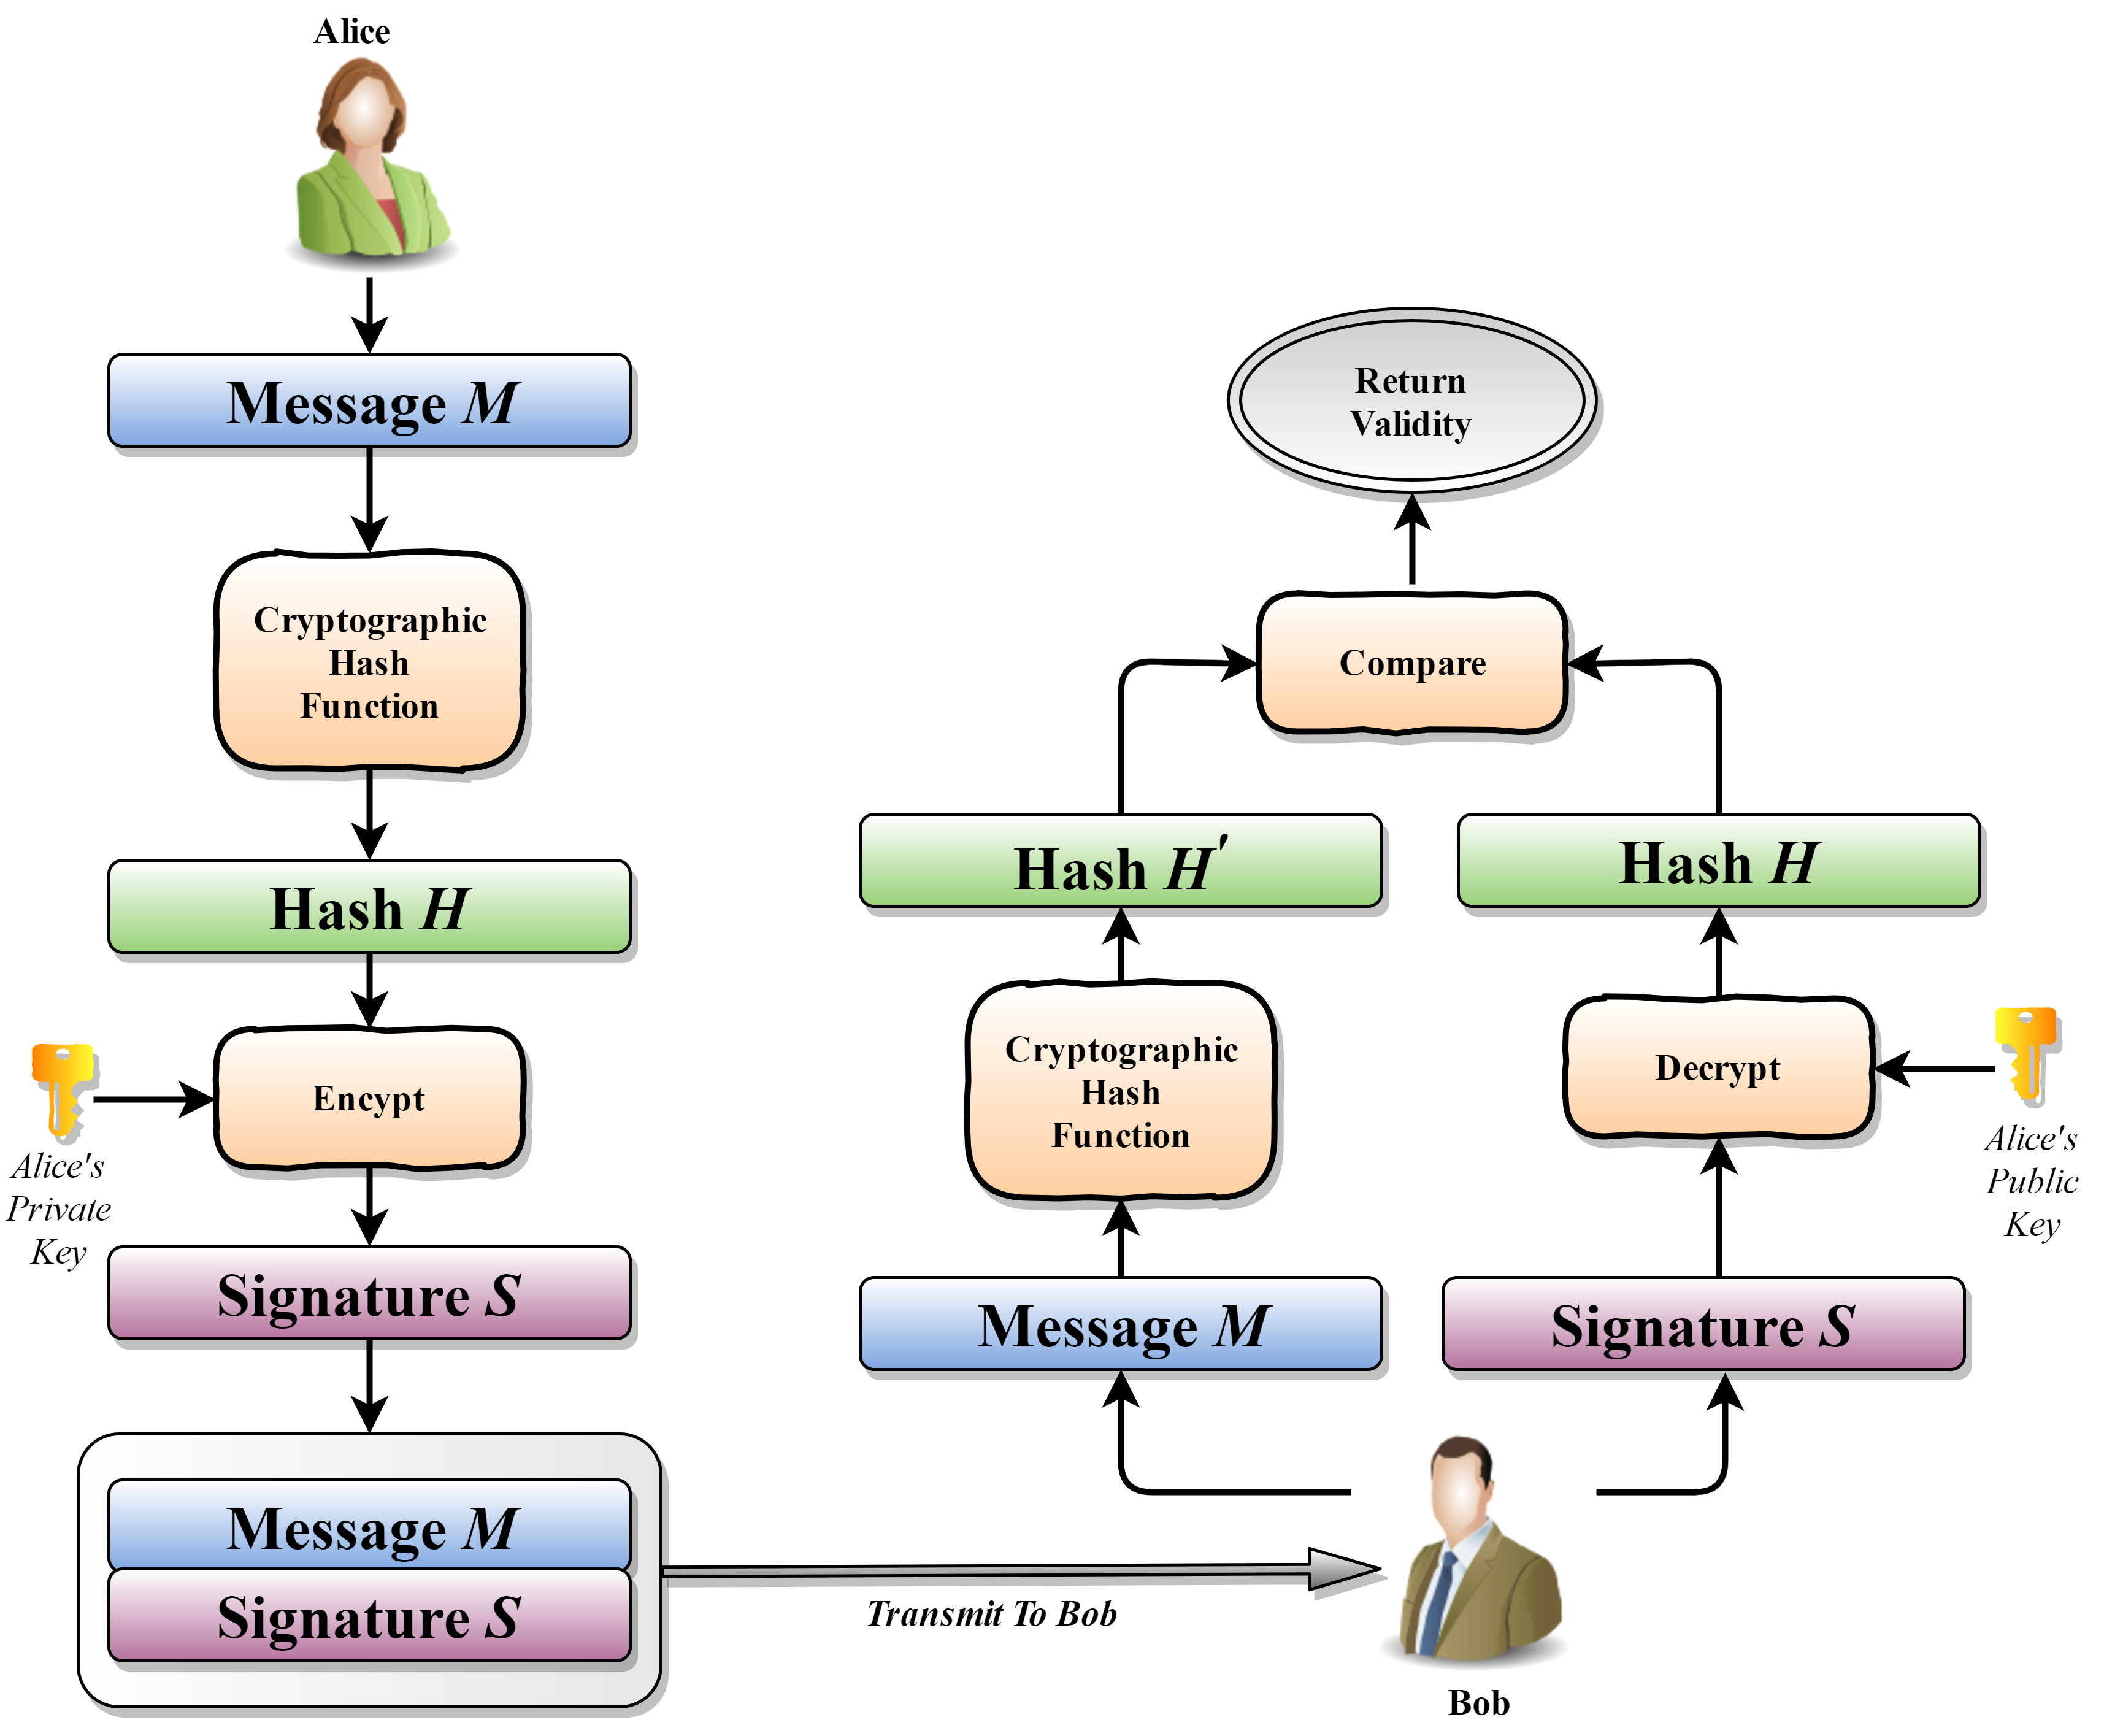
\includegraphics[width=\textwidth]{DigitalSignaturemod}
    \caption{Process of Digital Signature }
    \label{fig:Digital Signature}
\end{figure}

The figure \ref{fig:Digital Signature} shows the process of Digital signature. When Alice requires sending a message $M$, she first calculates hash $H$ of that message by using some predefined cryptographic hash function. The hash function produces a fixed size digest for a message which should be unique to avoid a collision. Then Alice encrypts the hash by using her private key and generates a signature $S$ for message $M$. The message $M$ along with signature $S$ is transmitted to the Bob, who is a potential verifier.

To verify the signature, Bob first calculates hash $H^\prime$ of the received message. Parallely he decrypts the signature $S$ by using Alice's public key, which should produce the hash $H$, which was calculated by Alice. Then Bob matches both the $H$ and $H^\prime$ and determines the validity of the signature which is true if $H = H^\prime$ and false if $H \neq H^\prime$. 

From the above example, we can analyze the security services provided by the Digital signatures. The collision resistant hash function produces unique digest for each message so the verifier can detect even a small change in the message. Hence the integrity is preserved in Digital signature. It is not possible to produce forged signature without knowing Alice's private key. Therefore verifier can rely on the authenticity of the message. The (private key, public key) pair is unique for Alice so she cannot deny her signature. Therefore the non-repudiation is also provided by Digital Signature. 

But along with the validity, Bob also gets to know the identity of Alice as her unique public key was used in validating the signature. As anyone can verify the signed message, the verifier also gets the identity of the signer and by using various messages signed by a signer can be used for profiling attack. Hence it is clear that the Digital signature does not provide confidentiality or privacy to the signer.
 
The Digital Signatures are widely used to ensure authenticity and already replacing traditional handwritten signatures. The RSA, ElGamal and Elliptic Curve algorithms are most popular asymmetric cryptographic algorithms used for Digital signatures. The Digital signatures are used in the field of web services and digital transactions along with signing electronic messages and documents.

\subsection{Public Key Infrastructure (PKI)}
Achieving authentication in a public key cryptosystem was one of the challenging problems. As a malicious user can easily masquerade as some other entity by using its public key. To overcome this problem, the concept of Public Key Infrastructure (PKI)\index{Public Key Infrastructure} \nomenclature{PKI}{Public Key Infrastructure} was introduced, which uses an application of Digital signatures. The PKI is a collection of policies and procedures required to create and manage digital certificates based on public key cryptography. The objective of PKI is to establish a relationship between an entity's cryptographic identity (e.g. public key) and non-cryptographic identities or attributes (like name, email, designation, etc.). Digital signatures are used in establishing such relationship. This link can be established using digital certificates by having trust between certified entity and issuer of the certificate. Using this certificate, a user can verify that the public key he is using for encryption, actually belongs to the entity which it claims to be. Masquerading as some other entity is not possible because the certificate can be easily validated in PKI. In short, the PKI solves the authentication problem in the public key cryptosystem. A simple Public Key Infrastructure includes following elements.
\subsubsection{Digital Certificate} A Digital Certificate\index{digital certificate} $cert_{CA \rightarrow A}$ is formed by PKI when it signs a message containing the cryptographic identity of $A$ (public key of $A$) and non-cryptographic identity of $A$ like its name. Whenever $A$ presents (public key of $A$, $cert_{CA \rightarrow A}$) to a verifier, the certificate can be verified that $cert_{CA \rightarrow A}$ is a valid signature generated by $CA$ using the public key of $CA$. The basic idea behind this is, $CA$ is a trusted by verifier that it will not certify invalid link between cryptographic and non-cryptographic identities. So $cert_{CA \rightarrow A}$ can be used to prove that the public key provided in the certificate $cert_{CA \rightarrow A}$, actually belongs to $A$. The Digital Certificate comes with an expiration time, and the certificate expires after that if it is not renewed.

\begin{figure}[h]
    \centering
    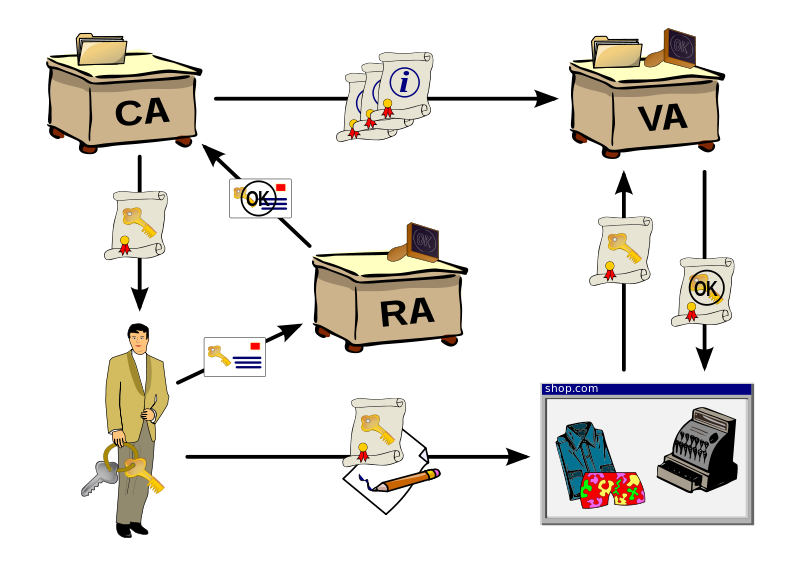
\includegraphics[width=\textwidth]{PKI}
    \caption{Public Key Infrastructure (PKI) }
    \label{fig:PKI}
\end{figure}

\subsubsection{Registration Authority (RA)} The fundamental objective of Registration Authority\index{registration authority(RA)} is to ensure valid registration of an entity. If an entity wants a digital certificate, then it required registering at registration authority. The registration authority verifies the validation of information provided to it and authenticate the entity making the request for the digital certificate. If everything is correct, then it sends a request to the Certificate Authority to issue a certificate for registered entity.
\subsubsection{Certificate Authority (CA)} The Certificate Authority\index{certificate authority(CA)} provides digital certificates to the entities enrolled by the Registration Authority. The Certificate Authority enables the user of PKI to rely on the public key in the certificate. It also acts as a trusted third party between the owner of a certificate and user on the certificate.
\subsubsection{Validation Authority (VA)} When a user of a certificate required to validate it, the Validation Authority\index{validation authority(VA)} provides validation. The Validation Authority receives all the certificate information from the Certificate Authority and used it to verify the certificate requested by the PKI user.\\
 
The PKI system also uses a certificate database which stores information of issued certificates, request for certificates and revoked certificates.

\subsubsection{Revocation of certificates} One of the important property of PKI is the ability to revoke any digital certificate which was issued in the past. There can be various reasons that a certificate required to be revoked. First is the expiration of time because each certificate has an expiration date and time. All the certificates which cross the expiration time and not renewed must be revoked after their expiration. Another reason is when the owner of a certificate changes his key, due to loss or theft of his private key. The certificate authority is responsible for the revocation of the certificate and sends the revocation information to validating authority so it can invalidate those certificates during verification.

\subsection{Privacy Issues}
In the earlier sections, we saw that the digital signatures provide security services like integrity, non-reputation, etc. The PKI also provides authentication by using trust-based systems. But while providing authenticity of the signer, digital signature or more generally PKI systems jeopardize user privacy. A digital signature of a user $A$ on some document $M$, when $A$ is in possession of PKI Certificate ($A$, public key of $A$, $cert_{CA \rightarrow A}$), reveals his identity to all the verifiers. Also when multiple of these digital signatures along with the signed messages by same user $A$, in different contexts, can be linked to him. It reveals much more information of the user. For example, a collection of multiple messages signed by the same user can be used for profiling of the signer. 
 
The PKI based authentication service provides one general solution to overcome this problem which is Anonymous Certificates. During generation of these anonymous certificates, CA verifies the identity of $A$, but the signature certificate $cert_{CA \rightarrow A}$ issued by CA on the public key of $A$, only contains (public key of $A$, $cert_{CA \rightarrow A}$). Where traditional certificates contain (non-cryptographic information of $A$, public key of $A$, $cert_{CA \rightarrow A}$). By using those anonymous certificates, it is not possible to obtain non-cryptographic information of a user directly from the certificate $cert_{CA \rightarrow A}$. But those anonymous certificates still provide the public key of a signer to all the verifiers. This information can be used to link a signer with the messages he signed and can be misused. 
 
The digital signatures and PKI certificates do not provide liberty to the user to maintain his privacy. The privacy of the user is sacrificed to obtain authenticity in those schemes. The next section introduces a new scheme which can provide authentication while preserving the privacy of the signer.

\section{Group Signatures: Authentication with Privacy}
As the previous section remarks, there are some shortcomings while using digital signatures and PKI based authentication in particular with regard to unlinkability and anonymity. But the unforgeability property of digital signatures provides undoubtedly authentication service. To accomplish all the security properties, especially anonymity with authentication some improvements are required in the digital signature scheme. The improved system needs to implement authentication like digital signature while preserving the privacy of the signer. The group based authentication systems are the best alternative which can provide all the security services as of digital signatures while protecting the privacy of the signer and providing him both anonymity and unlinkability.
\subsection{Group Based Authentication}
By using group based authentication\index{group based authentication} approach, a user can be authenticated on behalf of a group to which he belongs, rather than as an individual. In this procedure, the authentication process does not require any information that can be directly linked to an individual user. Instead, the user required to prove that he belongs to a particular group which has a certain degree of access for authentication. 

The group based authentication approach is suitable for achieving privacy because all the exposed information can only be linked to the group and not to the individual user. In this method, authentication is provided to the user if he can produce a proof of membership of the group. The group based authentication is usually implemented for access control where a user is often assigned to a group having permission to access certain resources, and by proving the membership of the group, an individual user gets access to those resources. In our context, however, the group based authentication can be implemented to digital signing techniques which in turn produces group signatures.
\subsection{Architecture of Group Signature}
The abstract idea of the group signatures\index{group signature} was first proposed by D. Chaum and V. Heyst in 1991\cite{chaum1991group}. The group signature uses group based authentication to protect the privacy of signers from possible verifiers. The brief idea of the functioning of group signatures is as follows. All the members of the group are considered as potential signers. Every signer is equipped with a unique private key. By using their private key, members can generate a signature for a document. The document gets signed on behalf of the group, which gives anonymity to the individual signer. 

Any verifier of the signature can verify it by using the public key of an entire group. Verifier only gets to know the public key of the entire group and cannot differentiate among two signatures as they are from the same member or not. Thus the signatures remain unlinkable to the verifiers. However, there exist a trusted party possessing the private key of the group generally called as the Group Manager, which can associate the signature to its original signer by using the private key of the group. Because the trusted third party can link the signature to its original signer, signers can not misuse the power of signing anonymously. Now we will discuss the detailed architecture of group signature scheme.

The architecture of group signature consists of four key elements in it. The Group, Group Manager, Group members, and verifier of a signature.
\subsubsection{The Group}
The Group in the architecture of group signature is not only just a collection of people having a shared set of goals but also the mathematical group, which is an algebraic structure consisted of elements and operations among those elements denoted by $\mathbb{Z}^*_n$. Each member of the group can be considered as a mathematical element, and certain operations are defined depending on the scheme of the group signature. The Group provides a mathematical foundation for the architecture of group signature scheme. Various operations of the scheme are implemented using the properties of a mathematical group. 

The mathematical structure of a group also helps to determine and prove the security requirements needed for implementation of group signature scheme. Usually, a group is formed by the Group Manager via creating essential elements required for it. Each group has a public key and private key similar to digital signatures. The private key is used for generation of private keys of the group members. Also, the private key of a group can be used to link a signature to its original signer. Therefore the private key of the group is kept secret and generally controlled by the Group Manager. The public key of the group is used for verification of the signature by many verifiers. The public key is accessible by any member of the system so it required being proved that the public key of a group cannot be misused for various attacks.
\subsubsection{Group Manager}
The Group Manager can be a single authority or faction of different authorities. The Group Manager is responsible for creation and continuance of the group. To create a group, the Group Manager choose a private key and specifies public key parameters. After the establishment of the group, Group Manager can join members in the group by providing them membership certificates. The private key of the group is required for generating a membership certificate. 

The private key of the group is also required for opening the signatures. The opening of a signature means associating the signature with its signer member or revoking identity of a signer. In some group signature schemes, the Group Manager can also revoke membership certificates of members. The revoked member then cannot generate a valid signature. The Group Manager is a trusted party in the group signature scheme, and if the Group Manager is compromised, then the group signature may not be considered as secure.
\begin{figure}[h]
    \centering
    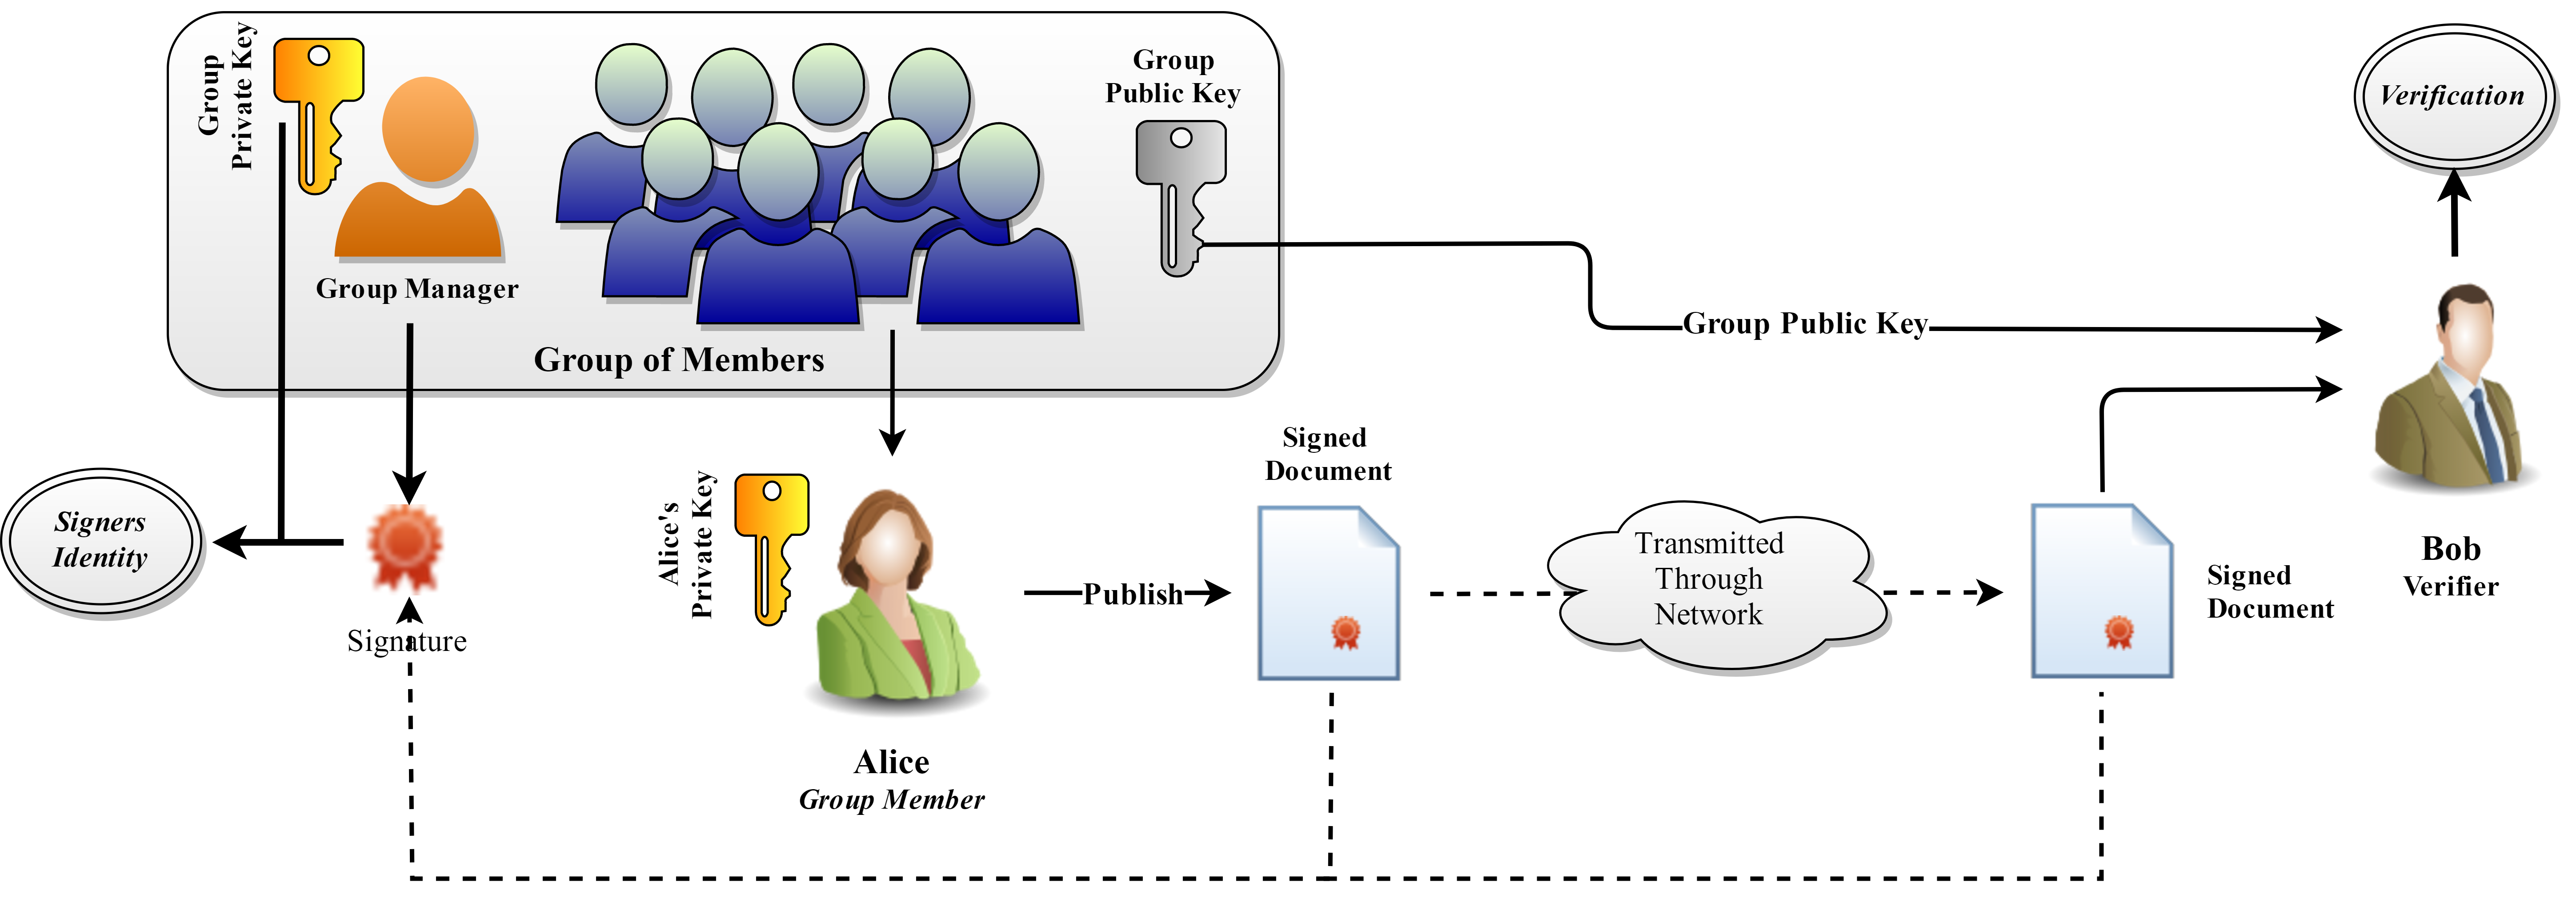
\includegraphics[width=\textwidth]{GroupSignature}
    \caption{Architecture of Group Signature }
    \label{fig:GroupSignature}
\end{figure}
\subsubsection{Group members}
The group member is the main beneficiary of the group signature scheme. The member joins the group by accepting a membership certificate which is required for obtaining private key of the member. After getting the membership certificate, a member can generate a signature for an arbitrary message. The signed message then transmitted to the receiver without disclosing the identity of the signer. The verifier of the message uses the public key of the group to verify issued group signature. 

The verification process proves that the signer is a valid member of the group, but the identity of the individual signer remains hidden from the verifier. Group Manager can open an issued signature. Therefore, it prevents any misuse of the power of anonymity and unlinkability provided to a member. The number knows that a disputed signature can be linked to its original signer.
\subsubsection{Verifier}
A verifier is an entity which authenticates the validity of a signature. To check the validity of a signature, the verifier uses the public key of the group, but the original signer of the signature cannot be known to a verifier. Instead, he only gets to know that the signer of the of a certain signature is a member of the group or not. No other information is known to the verifier. Therefore, he cannot extract information about any signer member.  

\subsubsection{Differences to PKI and Digital Signatures}
The group signature scheme appears similar to PKI-based authentication, but there is a significant variation between those two schemes. The Certificate Authority (CA) in PKI system, works similarly as Group Manager in group signature scheme. They both issues new certificate to users and have the ability to revoke the membership of a user. But the key difference between CA and Group Manager is that the certificate issued by CA contains the public key and some non-cryptographic information of the user where a certificate issued by Group Manager contains private key of the user and no other information. The certificate issued by CA is purposefully designed to be distributed publicly and the certificate issued by Group Manager must be retained secure and secret and should not be revealed by any group member.

The group signatures are different than the digital signatures in many ways. First, there is no public key required for group members whereas a public is needed for each user in the digital signature scheme. Instead, the group’s public key which is created by Group Manager is used for verification purpose and commonly used for verification of signatures, generated by all the group members. But still, the group signatures are publicly verifiable alike digital signatures.

The fundamental differences between ordinary signatures like digital signatures and group signatures is group signatures offer a guarantee of preserving the privacy of a user along with providing all the security services present in digital signatures. The public verification of group signatures does not leak any information of the signer during verification. The verifier authenticates signature based on information which only shows the status of membership of a signer, in the group. 

In group signatures, verifiers do not have the capability to recognize exact signer of a given signature. Instead, this ability is given to the Group Manager, which is a trusted authority. This unique combination of unlinkability and traceability not only gives signer the freedom to sign anonymously but also forces the responsibility of not misusing the power of anonymity. The misuse of a signature can be traced back to its original signer by   Group Manager, and sometimes the Group Manager can revoke the membership of such signer from the group. From above discussion, it can be seen that the group signatures provide greater functionality and applicability as compared to digital signatures.
\subsection{Security requirements of Group Signatures}
As the group signature provides authentication similar to digital signature it expected to provide all the security features available in the digital signature schemes. The group signatures are an enhancement to digital signatures required not only security features as of digital signatures but also some new specifications of its own, mainly due to the task of protecting the privacy of the signer. Several authors proposed these requirements for making the group signature scheme as secure as possible. All these requirements are needed to be proved correct by using mathematical basis and principals. A system implementing group signature must use number theoretical concepts not only to provide authentication but also to preserve privacy while following those security requirements. 
\subsubsection{Correctness}
Correctness\index{correctness} is the most fundamental property for group signature. The scheme having correctness property require always to generate a signature that can be verified correctly. That means legitimate signatures should have a negligible probability of identified as forged signature. The correctness property in a group signature can only be implemented by using mathematical proofs. There must be an accepted mathematical proof shows that the signing algorithm always creates such signatures which on verification gives accurate results and there is an only negligible possibility of false positive or negative.
\subsubsection{Unforgeability}
The unforgeability\index{unforgeability} property first introduced simultaneously with group signature scheme of D. Chaum \cite{chaum1991group}. It is similar to unforgeability of digital signatures. The unforgeability property permits only valid group member possessing a valid private key, to produce a legitimate signature and no one other can create such signatures. It is assumed that the private key of the signing member is safe and remain unknown to any attacker. The unforgeability property protects from chosen message attack in which an attacker might be able to produce valid group signature for a message selected from messages signed by a valid group member.
\subsubsection{Anonymity and Full Anonymity}
While proposing the first concept of group signature, D. Chaum considered anonymity\index{anonymity} to be a core property of group signature\cite{chaum1991group}. The anonymity requires that no one including verifiers of signature and other group members can be able to identify original signer of a signature, except for valid opening entity possessing a secret key. It implies that for a group of three members, a member who didn't sign, should not be able to identify which one of remaining two members was the signer of said signature. The property also assumes that the secret key for opening is secure and in possession of trusted authority who will not misuse it.

The strict model of Beller first introduced the concept of full anonymity\cite{bellare2003foundations}. The full anonymity\index{full anonymity} assumes that the private key of the signer is known to an attacker. And in such case too, it should not be possible to decide whether a given signature is from a particular signer or not. The main difference between anonymity and full anonymity is knowledge of private keys of a set of group members.
\subsubsection{Unlinkability}
The unlinkability\index{unlinkability} prevents to identifying any relation between two signatures. Beller introduces the unlinkability as a requirement for group signature\cite{bellare2003foundations}. The concept of unlinkability is associated to anonymity in some way. The unlinkability in group signature requires that it should not be possible to decide, whether two given signatures are from the same user or not. This property protects primarily from profiling attacks in which multiple messages from the same number are used for gathering information of members.
\subsubsection{Exculpability}
The concept of exculpability\index{exculpability} in group signature was introduced by Ateniese, as a variation of unforgeability\cite{ateniese1999some}. The requirement states that it should be impossible to create a valid signature for any member including Group Manager, which can be traced back to some other member. The exculpability defends a member from possible framing. When such property is present in group signature any signer can not be framed for signing a signature which he didn't sign. It also stops Group Manager from possible cheating and increases the trustworthiness of such authorities.
\subsubsection{Traceability}
The concept of traceability\index{traceability} was introduced while proposing the concept of group signature by D. Chaum\cite{chaum1991group}. The traceability is required for avoiding misuse of anonymity by the group members.  Any signature must be able to trace back to its original signer. The traceability also needed in following two scenarios. First, the group signatures cannot be able to produce a signature which gets verified as a legitimate but fails to identify its signer. Second, the tracing provides an output which is not the identity of the signer.
\subsubsection{Coalition Resistance}
Ateniese extends the traceability requirement for the group signature for resisting stronger attacks\cite{ateniese1999some}\index{coalition resistance}. This requirement checks that a colluding of multiple group member, should not be able to produce a valid signature by combining their keys. This requirement guarantees that a valid signature is always traceable to its one and only one signer. It also enhances the trust for the scheme and validity of a signature.
\subsubsection{Revocability}
The requirement of revocability\index{revocability} put a control on malicious nature of members. The revocability property enables the revocation of a member. Due to the implementation of this property, any member can be removed from the group at any time, and the signature produced by those member gets identified as invalid. The revocability puts a control on group member after they get their private key along with the power of creating anonymous signatures.
 
\subsection{Applications of Group Signatures}
The group signature has an enormous number of applications in real-world scenarios. The top applications of group signatures are in those scenarios where verifier does not require to know the actual identity of the signer. Instead, the knowledge of the membership status of the signer in an appropriate group is enough. Also, both the signer and verifier knows that the actual signer can be identified by trusted opening authority like Group Manager if needed.

Most beneficial utilization of group signatures can be found in conceal organizational structures like a company or government offices and administration. For example, an officer of government is trusted to issue orders, publish public statements, press releases, sign contracts and authorize financial transactions on account of the government. When group signatures used for this purpose, the actual identity of the officer will not be exposed, protecting him from revealing his identity to various parties involved in such matters. In this situation, the group signature not only protects the signing officer from threats or blackmailing but also helps to prevent corruption in the government.
However if such officer is found to be abusing his authority like signing illegal contracts or allowing illegal financial transactions, his identity can be revealed by using the Opening algorithm of the group signature. This opening can only be done by a trusted senior and high ranking officer so that the misuse of anonymous signing can be avoided. This opening procedure protects the organization from malicious employees to issue illegal documents or transactions. The opening of the signature can result in revocation of the signer, which can be achieved by the Revocation algorithm in group signature. The revocation algorithm not only eliminates the ability to produce valid signatures from the group member but also can be used to invalidate the valid signatures issued previously by the member.

Another application of group signatures is in online anonymous communication and identity escrow schemes. These schemes allow two parties to communicate anonymously. When a party misbehaves, its identity can be revealed by trusted opening entity. The group signature scheme can be converted to group identification scheme, where signature creation is transformed to the process of identification. This process of identification can be used to preserve the privacy of users, who identifies themselves to a third party. The paper of Lee explains the method of transformation of the group signature scheme to group identification scheme\cite{lee2010fiat}. This technique is useful in many circumstances, especially in outsourced service providing entities. An organization can acquire a service for its members, and members can utilize such service without giving their identity and just by using group identification scheme.

Some other applications of the group signatures are in electronic voting and bidding systems. In those schemes, a participant can place his bid anonymously without other parties identifying him. And when the auction concludes, the identity of winning party can be recognized by opening his signature. Some notable applications of group signature are in Vehicular Ad-Hoc Network (VANET)\nomenclature{VANET}{Vehicular Ad-Hoc Network} is proposed by Zhu et. el. where the identity of the vehicle is held secret while validating it\cite{zhu2013privacy}. The e-voting scheme of Lucas Malina can be used for implementing an electronic voting scheme where the identity of the voter can be kept secret and vote given by him cannot be linked to the voter\cite{malina2015secure}. 

The implementation of digital rights management can be achieved by applying group signatures. Group signature can be used for fingerprinting digital contents anonymously to protect the privacy of a user and still be able to identify the illegal distribution of such contents. 

This section proves that the group signature has infinite application in the real world, especially in the recent period where users are concerned with the preservation of their privacy, and service providers still need to authenticate the user.

\section{Motivation and Objective}
There are several approaches available which are able to provide authentication while protecting the privacy of the user. The group signature scheme is one of the best methods which provides a secure signing mechanism while protecting the privacy of the user by using the group based authentication approach. The digital signature scheme is found to be revolutionary in the digital documentation systems. Many modern documentation systems suffered from the problem of providing digital authentication before the emergence of the digital signature scheme. The digital signatures provide an efficient way to which the electronic documents can be signed and verified authentically, and it is impossible to replicate such signature to anyone except for the legitimate signer. While the digital signature solves the problem of digital authentication, it also issues concerns about the privacy of the signer.

In the paper based authentication system, the paper representing the message generally have signatures of the signer along with the seal of the signer. The seal is used to represent the position and power of the signer, but the advantages of the seal are they do not disclose any personal information about their holder. This approach protects the signer while providing the authentication because the signature alone contains very little information and the seal represents only the authority of the signer by which the verifier can assume that the signer possesses such authority to sign the document.

The digital signatures do not provide these kinds of features. Therefore all the information of the signer is always considered to be public. Also, a valid signature does not necessarily represent the authority of the signer. Therefore some issues left unsolved for the organizational structures like a company or government departments which are using the digital signature for digitally signing their documents.

The solution to such problems was provided by the approach of the group based authentication systems. The group based authentication can represent the authority of the members the combining and forming a group of people having similar or equal authorization. The group signature scheme uses a similar group based authentication system for signing the message. There are many group signatures schemes proposed which provide secure authentication with privacy, but many of these same have some drawbacks. A detailed discussion about some of these systems along with their shortcoming will be discussed in the next chapter.

There is a lot of scopes available for improvement of the group signature schemes. These improvements consist of improving correctness of the signatures, reduction of the computational time and cost for generation of the signature, dynamic addition as well as revocation of the group members. The enhanced distribution of the trusted authorities and an efficient correlation between them and provision of a verifiable proof which can verify the actions of these authorities are also some additional improvement required. These domains of the group signature scheme should be improved so that the group signature scheme should become robust and secure.

The objective of this dissertation is to find an efficient distribution of the trusted authorities so that the users of the group signature system does not need to put all their faith in a single authority. Also replacing the trusted tasks of the authorities with mathematical approved algorithms can reduce the requirement of the trust in the trusted authorities. The revocation mechanism is the important but least discussed topic in the group signature scheme. The implementation of revocation supporting scheme with not only required to be efficient but also secure and robust is also one of the objectives. 

The computational cost of the implementing group signature scheme is expected to be lower for better efficiency. Therefore the reduction of computational time and space in the implementation of a secure and efficient group signature scheme is also one major objective of this dissertation. 

\section{Organization}
The work of the dissertation presents an architecture for dynamic groups signature scheme with distributed authorities and supporting the dynamic revocation of the group members. The group signature scheme also reduces the computational cost for generating the signature. The organization of rest of this dissertation is in the following manner.
\subsubsection{Chapter 2}
Chapter 2 presents background information about the group signature schemes which include the classification of groups signatures schemes according to their architecture. The chapter to describes various groups signature schemes proposed earlier with a review of their advantages and shortcomings. These schemes are described on the basis of their mathematical assumptions. The chapter also provides a short review of similar approaches presented earlier for providing authentication while preserving the privacy of the user.
\subsubsection{Chapter 3}
The Chapter 3 of this dissertation provides an introduction to some number theory concepts which are essential in cryptographic as well as group signature systems. The chapter provides the formal definition of the groups, trapdoor permutation, hash functions and random oracle model along with a brief description of number theoretical assumptions on which the proposed group signature scheme relies. It also provides some discussion about zero knowledge proofs and the signature of knowledge (SoK).
\subsubsection{Chapter 4}
Chapter 4 contains proposed work for this dissertation. The proposed work is broken into four sections. The distribution of authorities section shows how the authorities in proposed group signature scheme are distributed and their working.  In the next section we are providing the formal definition of proposed group signature scheme, and then the architecture of the system is introduced. The details of the algorithms and their customization with working is provided in the model development section.

\subsubsection{Chapter 5}
Chapter 5 of this dissertation provides the analysis of proposed group signatures scheme from the security as well as performance point of view. The chapter discusses the functionalities provided by the proposed group signature scheme and their advantages. Then the security properties of this scheme are analyzed, and the scheme is compared with some important group signature schemes. The performance analysis of the scheme discusses the complexity of the algorithms in it.

\subsubsection{Chapter 6}
Finally, the dissertation concludes in Chapter 6. The chapter provides the conclusion of the work in this dissertation along with the future scope of the proposed group signature scheme, and then the references used in this thesis are listed.

\chapter{Literature Survey}\label{chp:lit.survay}
%Literature Survey
The first and foremost idea which considered preserving privacy while providing authentication was proposed by D. Chaum and V. Heyst in 1991 \cite{chaum1991group}. The signature model of Chaum uses group based authentication approach to implement authentication with privacy protection. Four different schemes were proposed by Chaum. Three of those schemes were undeniable signatures and a Group Manager required to communicate with every member of the group to identify the original signer. These schemes provided computational anonymity to signers. The fourth scheme was not undeniable and only provided theoretical anonymity based on selected information. Two of the proposed schemes required to calculate private key of the members beforehand that is before setting up the group. The schemes introduced by Chaum not only provided a conceptual idea of how group signature should be implemented but also provided some basic algorithms for group signature like sign, verify and open. After the introduction of group signatures, various schemes were proposed which not only improved group signature schemes of Chaum but also leads to having several additional functionalities for better application orientations. Those different schemes have varying functionality and limitations in them. The following section describes the classification of the group signature schemes based on their features.

\section{Classification of Group Signatures}\label{ClassificationGroupSignatures}
The classification of groups signature schemes can be done according to functionality present in them. All those schemes have some standard functions like group member having ability to generate a signature which can be verified in group based authentication system without revealing the identity of the signer. By using this basic principle, various types of group signatures were proposed. Some essential functionalities in those schemes are as follows.
\begin{itemize}
\item The ability of the schemes to generate a private key of a member after creation/setup of the group.
\item The capability to produce verifiable proof that a given signature can be linked to one and only one signer.
\item The ability of distribution of power possessed by Group Manager into multiple entities like separate entity for opening signature rather than Group Manager alone.
\end{itemize}

The classification of group signature in the section is based on functional properties present in the schemes. It also provides a high-level overview of algorithms present in group signature schemes. The classification given below includes almost all the major group signature scheme which existed till now.
\subsection{Static Group Signatures}
The static group signature scheme\index{static group signature scheme} is very primitive and straightforward signature scheme among all the group signature schemes. In static group signature scheme, the number of group members is fixed and decided at the beginning of the group and before the setup of the group. The private keys of the group members were computed before setup of the group and cannot be calculated after the setup. Therefore only fixed members are allowed in the static group signature scheme. 

The Group Manager in these schemes is almost always a single entity, bearing the responsibilities of computing the private keys of the group members, distribution of these private keys to the members and linking signature to their original signer. The formal definition of the static group signature is as follows. The definition and description of algorithms are based on the model of static group signature proposed by Bellare, Micciancio, and Warinschi \cite{bellare2003foundations}.
\nomenclature{gpk}{group public key}
\nomenclature{gsk}{group private key}
\nomenclature{mpk}{member's private key}
\begin{definition}[Static group signature scheme] A static group signature scheme consists of following four algorithms.\\
\textbf{SetUp:} The randomized \texttt{SetUp} algorithm takes input security parameters $(1^k, n)$ where $k\in \mathbb{N}$  and $n$ as the number of group members $n\in \mathbb{N}$ and generates a tuple $(gpk, gsk, mpk)$ where $gpk$ is group public key, $gsk$ is group private key, $mpk$ is member's private key is an array with $mpk\lbrack i \rbrack$ is the private key of the member $i$.\\	
\textbf{Sign:} The randomized algorithm \texttt{Sign} produces a signature $S$ for a message by taking input $(mpk, M)$ where $mpk$ is member private key and $M$ is the message.\\
\textbf{Verify:} The deterministic signature \texttt{Verify} algorithm determines the validity of a signature on a message $M$ by taking input $(gpk, M, S)$ where $gpk$ is group public key, $M$ is the message, $S$ is signature and returning \texttt{true} for valid and \texttt{false} for invalid signature.\\
\textbf{Open:} The deterministic algorithm \texttt{Open} returns $mpk$ that is members private key by taking input $(gsk, S)$ where $gsk$ is group private key and $S$ is the signature for a message. It is required that the validity of the signature must be true by \texttt{Verify} algorithm to return correct $mpk$.
\end{definition}

\begin{figure}[h]
    \centering
    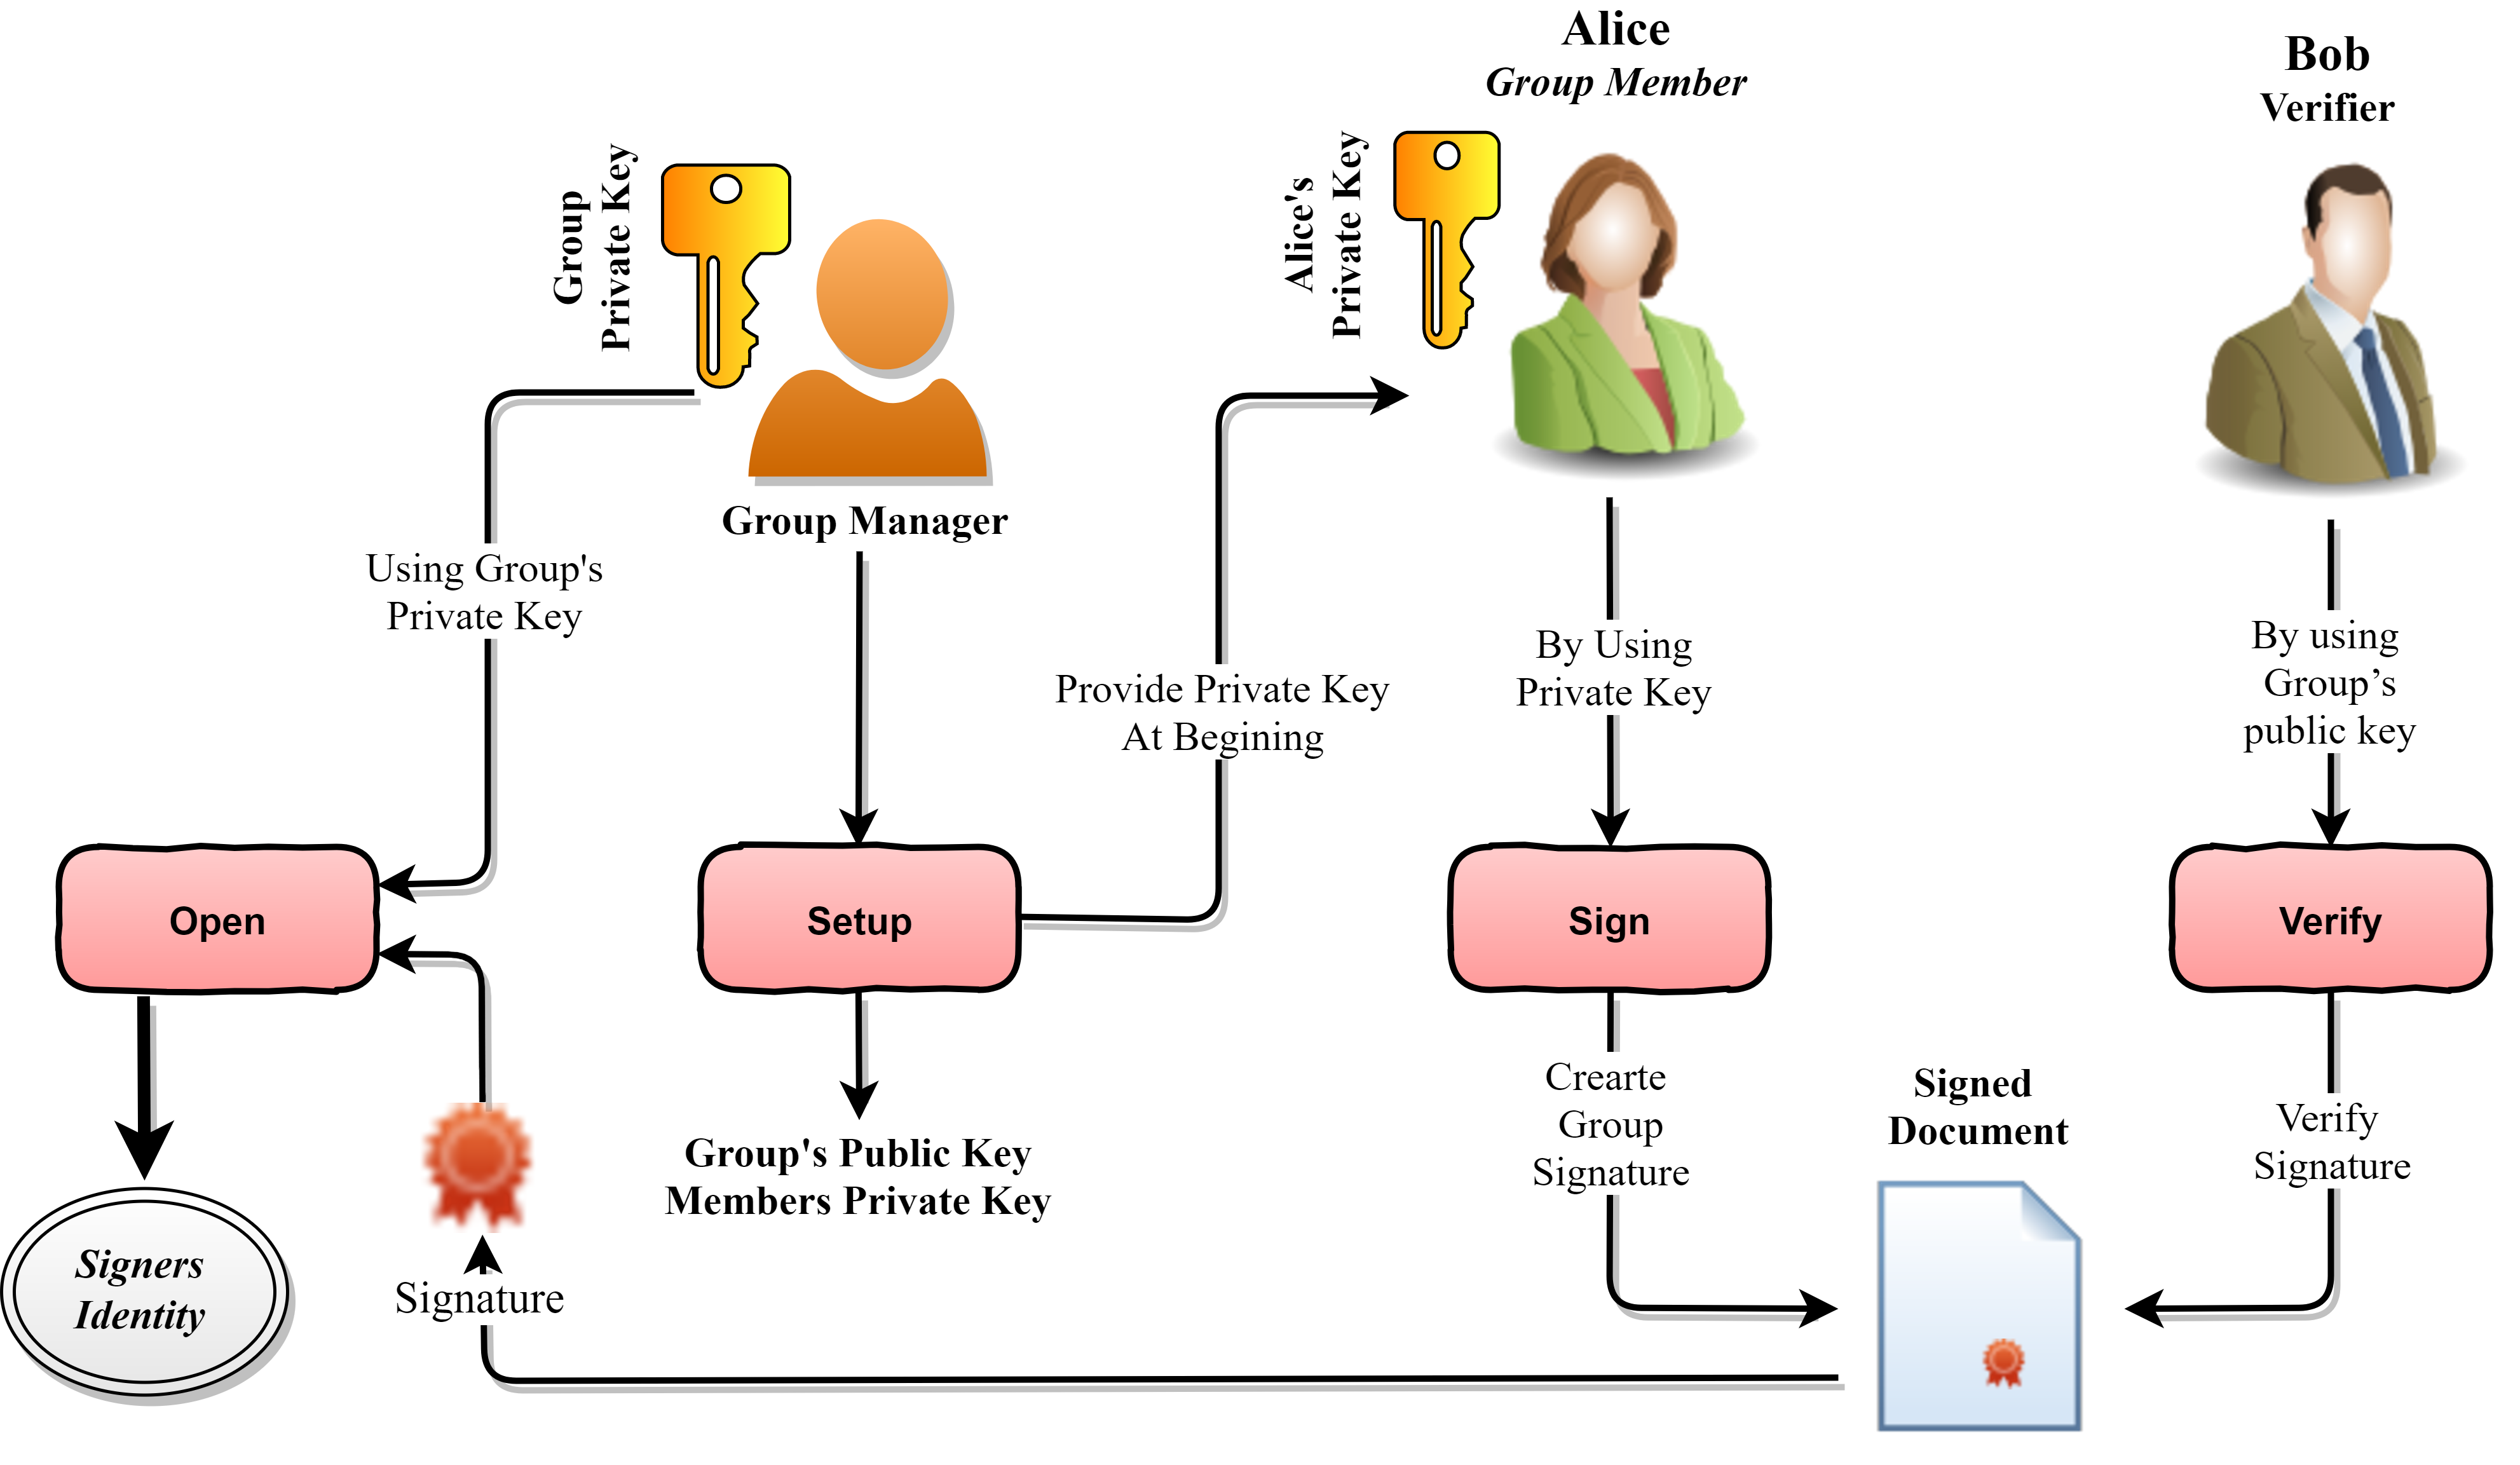
\includegraphics[width=\textwidth]{StaticGroupSignature}
    \caption{Static Group Signatures Scheme}
    \label{fig:Static Group Signatures Scheme}
\end{figure}

The figure \ref{fig:Static Group Signatures Scheme} describes the procedure of static group signature scheme. First, the Group Manager generate Group Private key, Group Public key and private keys of all the members. Group Manager then distributes the private keys of members to them securely. Once the members get their private key, they can generate the signature for any message. Alice as a group member receives her private key from Group Manager. To sign a message, Alice uses her private key to produce the signature for the message and the message along with the signature is transmitted to Bob, who is a verifier via an insecure channel. To verify the signature of the message, Bob executes Verify algorithm which determines the validity of the signature but does not disclose any information about signer, in this case, Alice. To link the signature to its original signer, the Group Manager executes the Open algorithm which returns the identity of the signer, in this case, the identity of Alice. 

Note that although static group signature schemes have a fixed number of members, these schemes can offer the functionality of revocation of the members which allows removing members from the group (but can not add any new members).

\subsection{Dynamic Group Signatures}\label{sub:Dynamic Group Signatures}
The static group signatures have the limitation of not only fixed number of members but also the requirement of deciding their number at the commencement of the group. Many applications of group signature are not able to be implemented because of such limitations of static group signatures. Those applications require the ability of addition of members at any time after commencement the group. The dynamic group signature scheme does not have limitations of fixed members determined at the beginning of group like static group signatures.

In the dynamic group signature scheme\index{dynamic group signature scheme}, the Group Manager can add any number of members at any time after commencement of the group. It implies that the private key of a new member can be generated after the creation of the group. The dynamic group signature scheme has an additional join protocol in extension to the four protocols in static group signatures. The join protocol is a protocol between Group Manager and a user who wishes to become a member of the group. To implement this dynamic member join protocol, the remaining algorithm in group signature, especially the setup algorithm required to be altered.

Similar to static group signatures, some dynamic group signature may offer the functionality of revocation of the group members. The revoked members cannot produce a valid group signature. These schemes have a true dynamic-ness in them, as they can add and remove any member of the group at any time. The following section provides the definition of dynamic group signature scheme and description of the algorithms in it.

\begin{definition}[Dynamic group signature scheme]A dynamic group signature scheme consist of following five algorithm/protocols.\\
\textbf{SetUp:} The randomized \texttt{SetUp} algorithm takes an input of security parameter $1^k$ where $k\in \mathbb{N}$ and generates a tuple $(gpk, gsk, List)$ where $gpk$ is group public key, $gsk$ is group private key, $List$ is a list of members of the group. The $List$ is empty at the commencement of the group.\\
\textbf{Join:} The randomized \texttt{Join} algorithm is a protocol between Group Manager and a user which takes an input of $gsk$ from Group Manager and produce $mpk$ which is members private key for the user making him a valid group member. It also adds the credentials of the user into the list like his $mpk$.\\
\textbf{Sign:} The randomized algorithm \texttt{Sign} produces a signature $S$ for a message by taking input $(mpk, M)$ where $mpk$ is member private key and $M$ is the message.\\
\textbf{Verify:} The deterministic signature \texttt{Verify} algorithm determines the validity of a signature on a message $M$ by taking input $(gpk, M, S)$ where $gpk$ is group public key, $M$ is the message, $S$ is signature and returning \texttt{true} for valid and \texttt{false} for invalid signature.\\
\textbf{Open:} The deterministic algorithm \texttt{Open} returns $mpk$ that is members private key by taking input $(gsk, S)$ where $gsk$ is group private key and $S$ is the signature for a message. It is required that the validity of the signature must be true by \texttt{Verify} algorithm to return correct $mpk$.
\end{definition}
\begin{figure}[h]
    \centering
    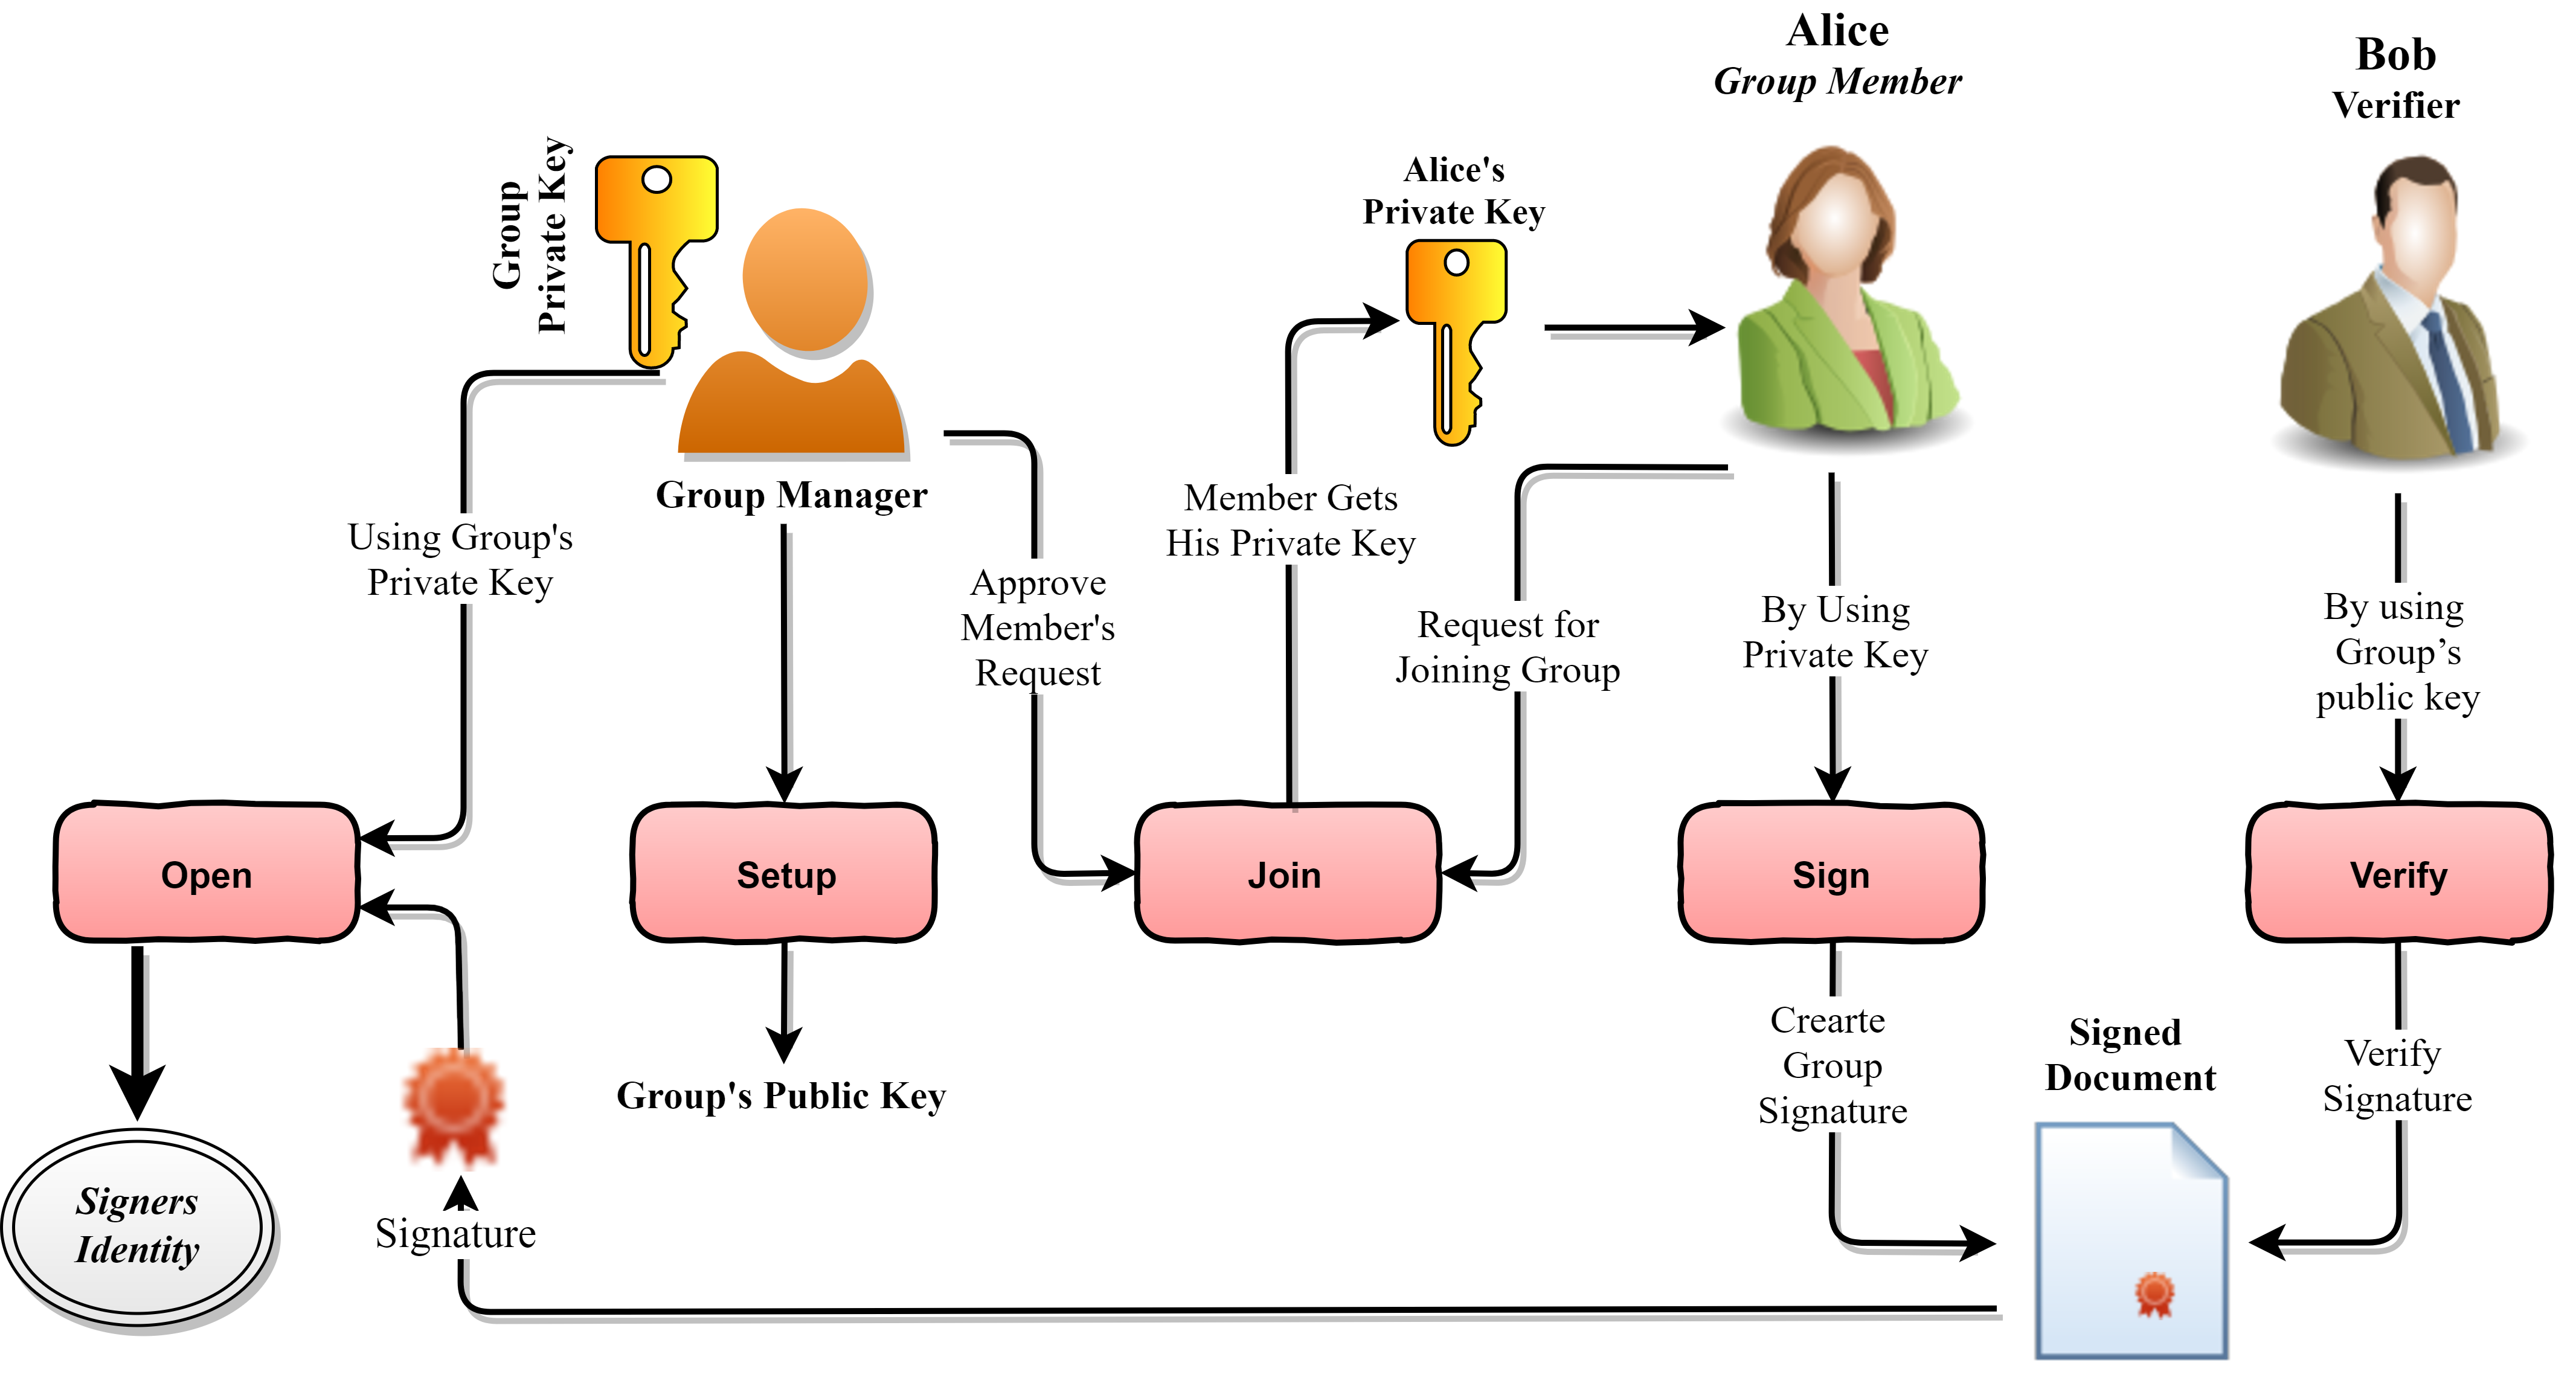
\includegraphics[width=\textwidth]{DynamicGroupSignature}
    \caption{Dynamic Group Signatures Scheme}
    \label{fig:Dynamic Group Signatures Scheme}
\end{figure}
The figure \ref{fig:Dynamic Group Signatures Scheme} describes the procedure of dynamic group signature scheme. Initially the Group Manager setup the group creating his private key and groups public key. When Alice as a user wants to join the group, she requests to the Group Manager by using the join protocol. The Group Manager then approves the request sent by Alice and the join algorithm provides a private key to the member, in this case, Alice and add his credential into the database. The Group Manager may or may not know the $mpk$ of member depending on the scheme, but as a trusted authority, Group Manager is supposed to be having knowledge of $mpk$ of all the members. After becoming the member of the group by getting her private key, Alice as a group member is now able to produce group signature by using sign algorithm for any message. After signing a message, Alice transmits the signed message along with the signature to Bob, who is a potential verifier via an insecure channel. To verify the signature of the message Bob executes the verify algorithm which determines the validity of the signature. Note that during the transmission of the message Alice not needed to show her name as sender or signer. It is also possible to publish the message to the intended receiver anonymously.

Note that although the dynamic group signature does not have a fixed number of members, theoretically the scheme always have an upper bound $n$ which denotes the maximum number of possible members in a group. It should be taken care that the upper bound $n$ should be large enough so that all the possible number of members can join the group without approaching its limit.
\subsection{Group Signature Schemes with Verifiable Opening}
\index{group signature schemes with verifiable opening}The group signatures have a unique property of not only preserving the privacy of the signer but also provide the power of traceability to a trusted authority. The trusted authority like Group Manager can associate a signature to its original signer by using his private key. But the opening of the signature is usually fall-back mechanism and infrequently used. The opening of the signature usually follows subsequent actions on the signer like his revocation form the group. In such cases, the actions of the opening entity like Group Manager are required to be completely selfless, and any member is not being accused falsely by the Group Manager. The trust level of the Group Manager needs not to be required of a very high level when there can be a mechanism of publicly verifiable proof. The group signature with publicly verifiable opening provides the same mechanism. 

In these group signature schemes when the opening of the signature is performed, the Group Manager not only provide the identification of the signer but also provide a publicly verifiable proof that any user can verify and conclude that the Group Manager is not falsely accusing any member, for a signature. The proof provided by Group Manager mathematically proves that the identity of the signer is in did the one whose signature Group Manager claim it to be. The functionality of the publicly verifiable proof can be implemented by improving or modifying the opening algorithm in group signature scheme. This modified opening algorithm provides a publicly verifiable proof along with the identification of the signer. An additional algorithm is required for judgment or verification of the proof given by the opening algorithm, which determines the truthfulness of the proof. This Judge algorithm should always be publicly accessible so that anyone can verify the sincerity of the proof. Following section provide the definition of the group signature scheme with variable opening and description of the algorithms in it.

\begin{definition}[Group Signature Schemes with Verifiable Opening] A group signature scheme with a variable opening is a static or dynamic group signature scheme with an improved opening algorithm and an additional judge algorithm for public verification of result of the opening algorithm.\\
\textbf{Open algorithm:} The deterministic algorithm \texttt{Open} produces output of pair (signer's identity $i$ and proof $\mathbb{T}$) it by taking input of $(gsk, S)$.\\
\textbf{Judge algorithm:} The deterministic algorithm \texttt{Judge} produces a result of validity of the proof, generated by the \texttt{Open} algorithm. That is \texttt{true} for valid and \texttt{false} for invalid proof, after taking the input of $(gpk, M, S, i, \mathbb{T})$ where $i$ is the identity of the signer and $\mathbb{T}$ is proof produced by the \texttt{Open} algorithm.
\end{definition}
\begin{figure}[h]
    \centering
    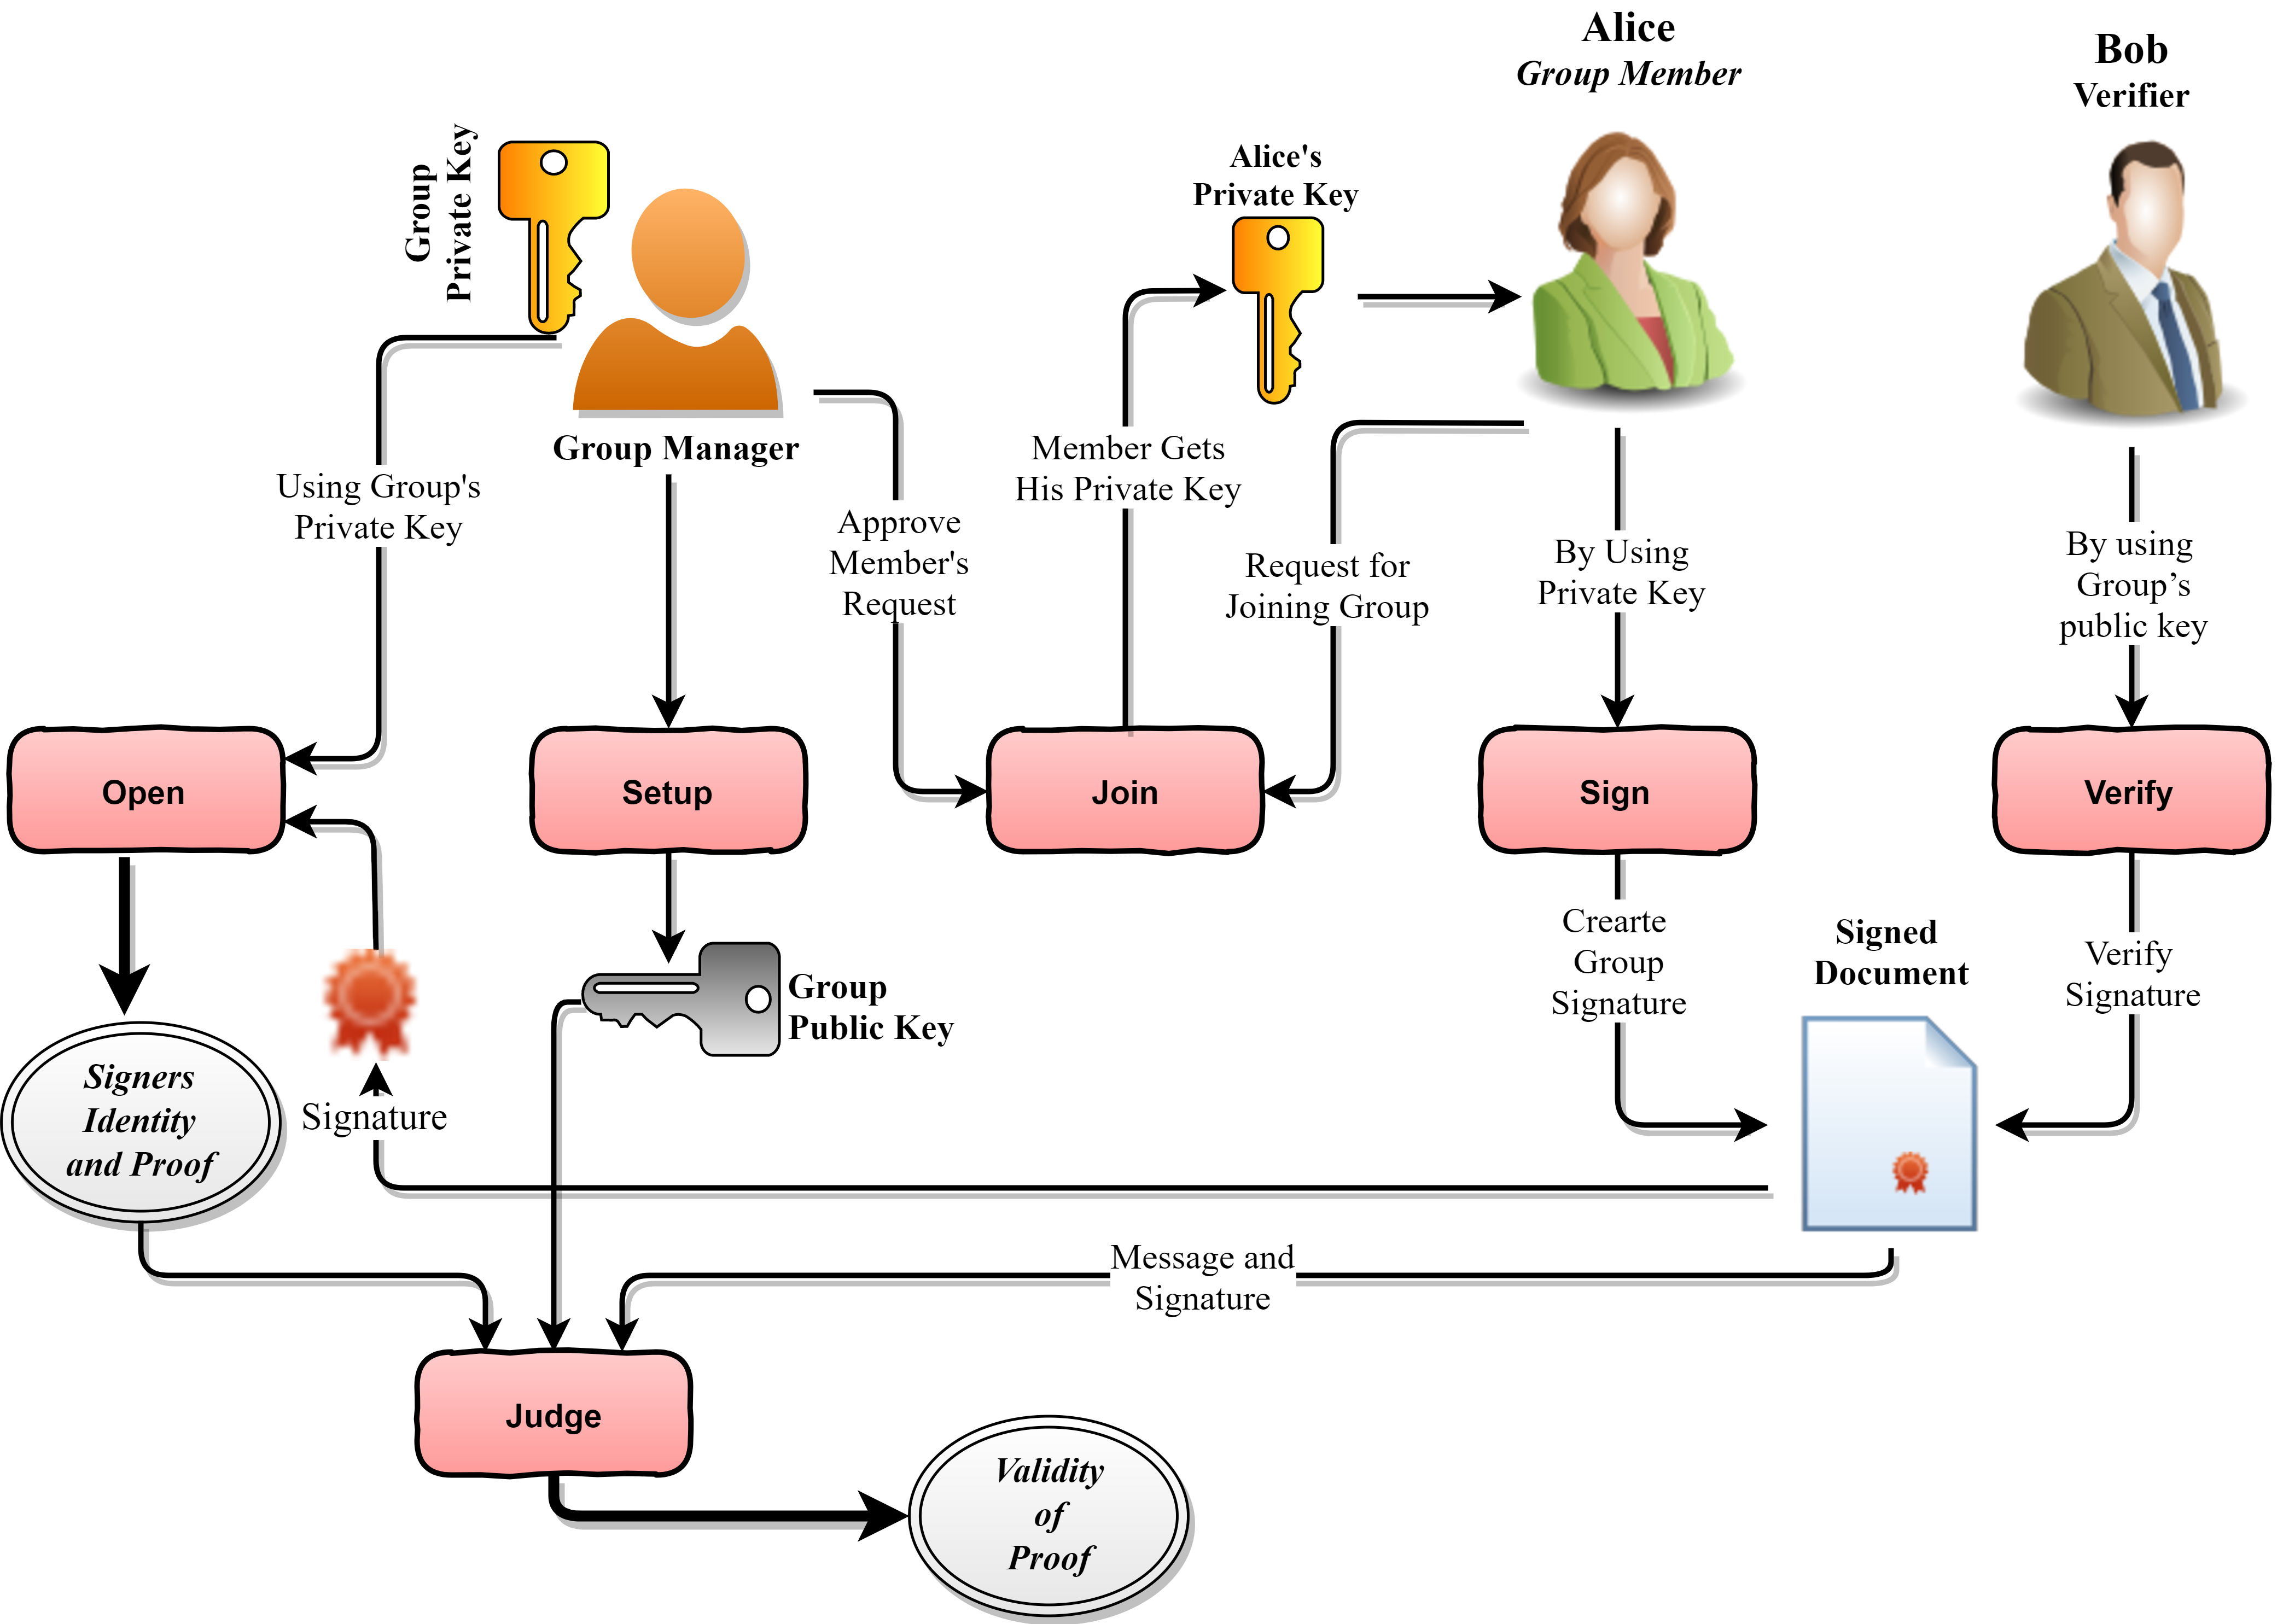
\includegraphics[width=\textwidth]{Publicverificableopeninggroupsignature}
    \caption{Group Signature Schemes with Verifiable Opening}
    \label{fig:Public verificable opening group signature}
\end{figure}
The figure \ref{fig:Public verificable opening group signature} shows the structure of publicly verifiable opening supported group signature scheme. In the figure, all the other components are similar to the dynamic group signature scheme and can be replaced with the static group signature scheme. The notable difference to those schemes is that the opening algorithm produces a proof along with the signer's identity. The supplementary algorithm Judge takes the input of the output of opening algorithm along with signature and message plus group public key and provides validity of the proof as an output. 

Note that the extension of the verifiable opening can be applied to both Static and Dynamic schemes because the extension only requires modification of opening algorithm which is present in both the schemes.

\subsection{Group Signature Schemes with Distributed Authorities}\label{sec:Group Signature Schemes with Distributed Authorities}
\index{group signature schemes with distributed authorities}The role of a Group Manager in a group signature scheme is one of the important roles as a trusted authority. In various schemes of group signatures, the Group Manager is responsible for various duties. To perform these functions, the members required to put a lot of trust in the Group Manager. Although we saw in previous schemes, Group Manager needed to provide publicly verifiable proof for an opened signature. It does not reduce the level of trust required in Group Manager's role. One important solution to those problems is to distribute the tasks of Group Manager among multiple separate entities. It helps in migrating the amount of trust in Group Manager and suites for some specific applications where trust is not required, and separation is necessary for architecture of the group signature scheme. 

The important tasks that a Group Manager is supposed to be responsible are, the generation of the private and public key of the group, opening the signature, revocation of the members in the revocation supported schemes, distribution of private keys of the members in static and joining of the member in dynamic schemes. All these tasks required in common is the private key of the group. So if the mathematical foundation of the group signature can be constructed in such a way that separate private keys are required for performing the tasks mentioned above, it is possible to distribute the role of Group Manager into various authorities. The essential functions of the distributed authorities are as follows.

The first task is the generation of the private and public key of the group, as well as the distribution of private keys to the members in static and joining the members in dynamic schemes, can be assigned to a separate authority called as the \texttt{Issuer}. An another authority can be assigned the task of opening the signature. This authority possesses a unique opening key, which can associate a signature to its signer. This type of authority is known as the \texttt{Opener}. If the scheme supports revocation of the members, the task of the revocation can be assigned to a separate authority called the \texttt{Revocator}. Some architecture may also suggest that when opening authority identifies the signer of a signature, it can also send a request to the revocation authority to revoke that member along with the identity of the signer and only then revocation authority can revoke such member.
\begin{definition}[Group Signature Scheme with Distributed Authorities]\label{def:Group Signature Scheme with Distributed Authorities}The group signature scheme with distributed authorities, is a static or dynamic group signature scheme in which \texttt{SetUp}, \texttt{Open} and \texttt{Join} algorithms are modified in such a way that different private keys are required for their execution.\\
\textbf{SetUp:} The randomized \texttt{SetUp} algorithm produces a tuple $(gpk, gsk\lbrack~\rbrack, list)$ by taking an input of security parameter $(1^k, k \in \mathbb{N})$ where $gsk$ is the private key of the authority is an array denoting $gsk\lbrack i \rbrack$ is a private key of the authority $i$.\\
\textbf{Join:} The randomized \texttt{Join} algorithm is a protocol between the issuer and a user which takes input $gsk\lbrack Issuer \rbrack$ and provide $mpk$ to the user which is his private key.\\
\textbf{Open:} The deterministic algorithm \texttt{Open} returns $mpk$ of signer member by taking input $(gsk\lbrack Opener \rbrack, S)$ where $S$ is the signature of a message.
\end{definition}
\begin{figure}[h]
    \centering
    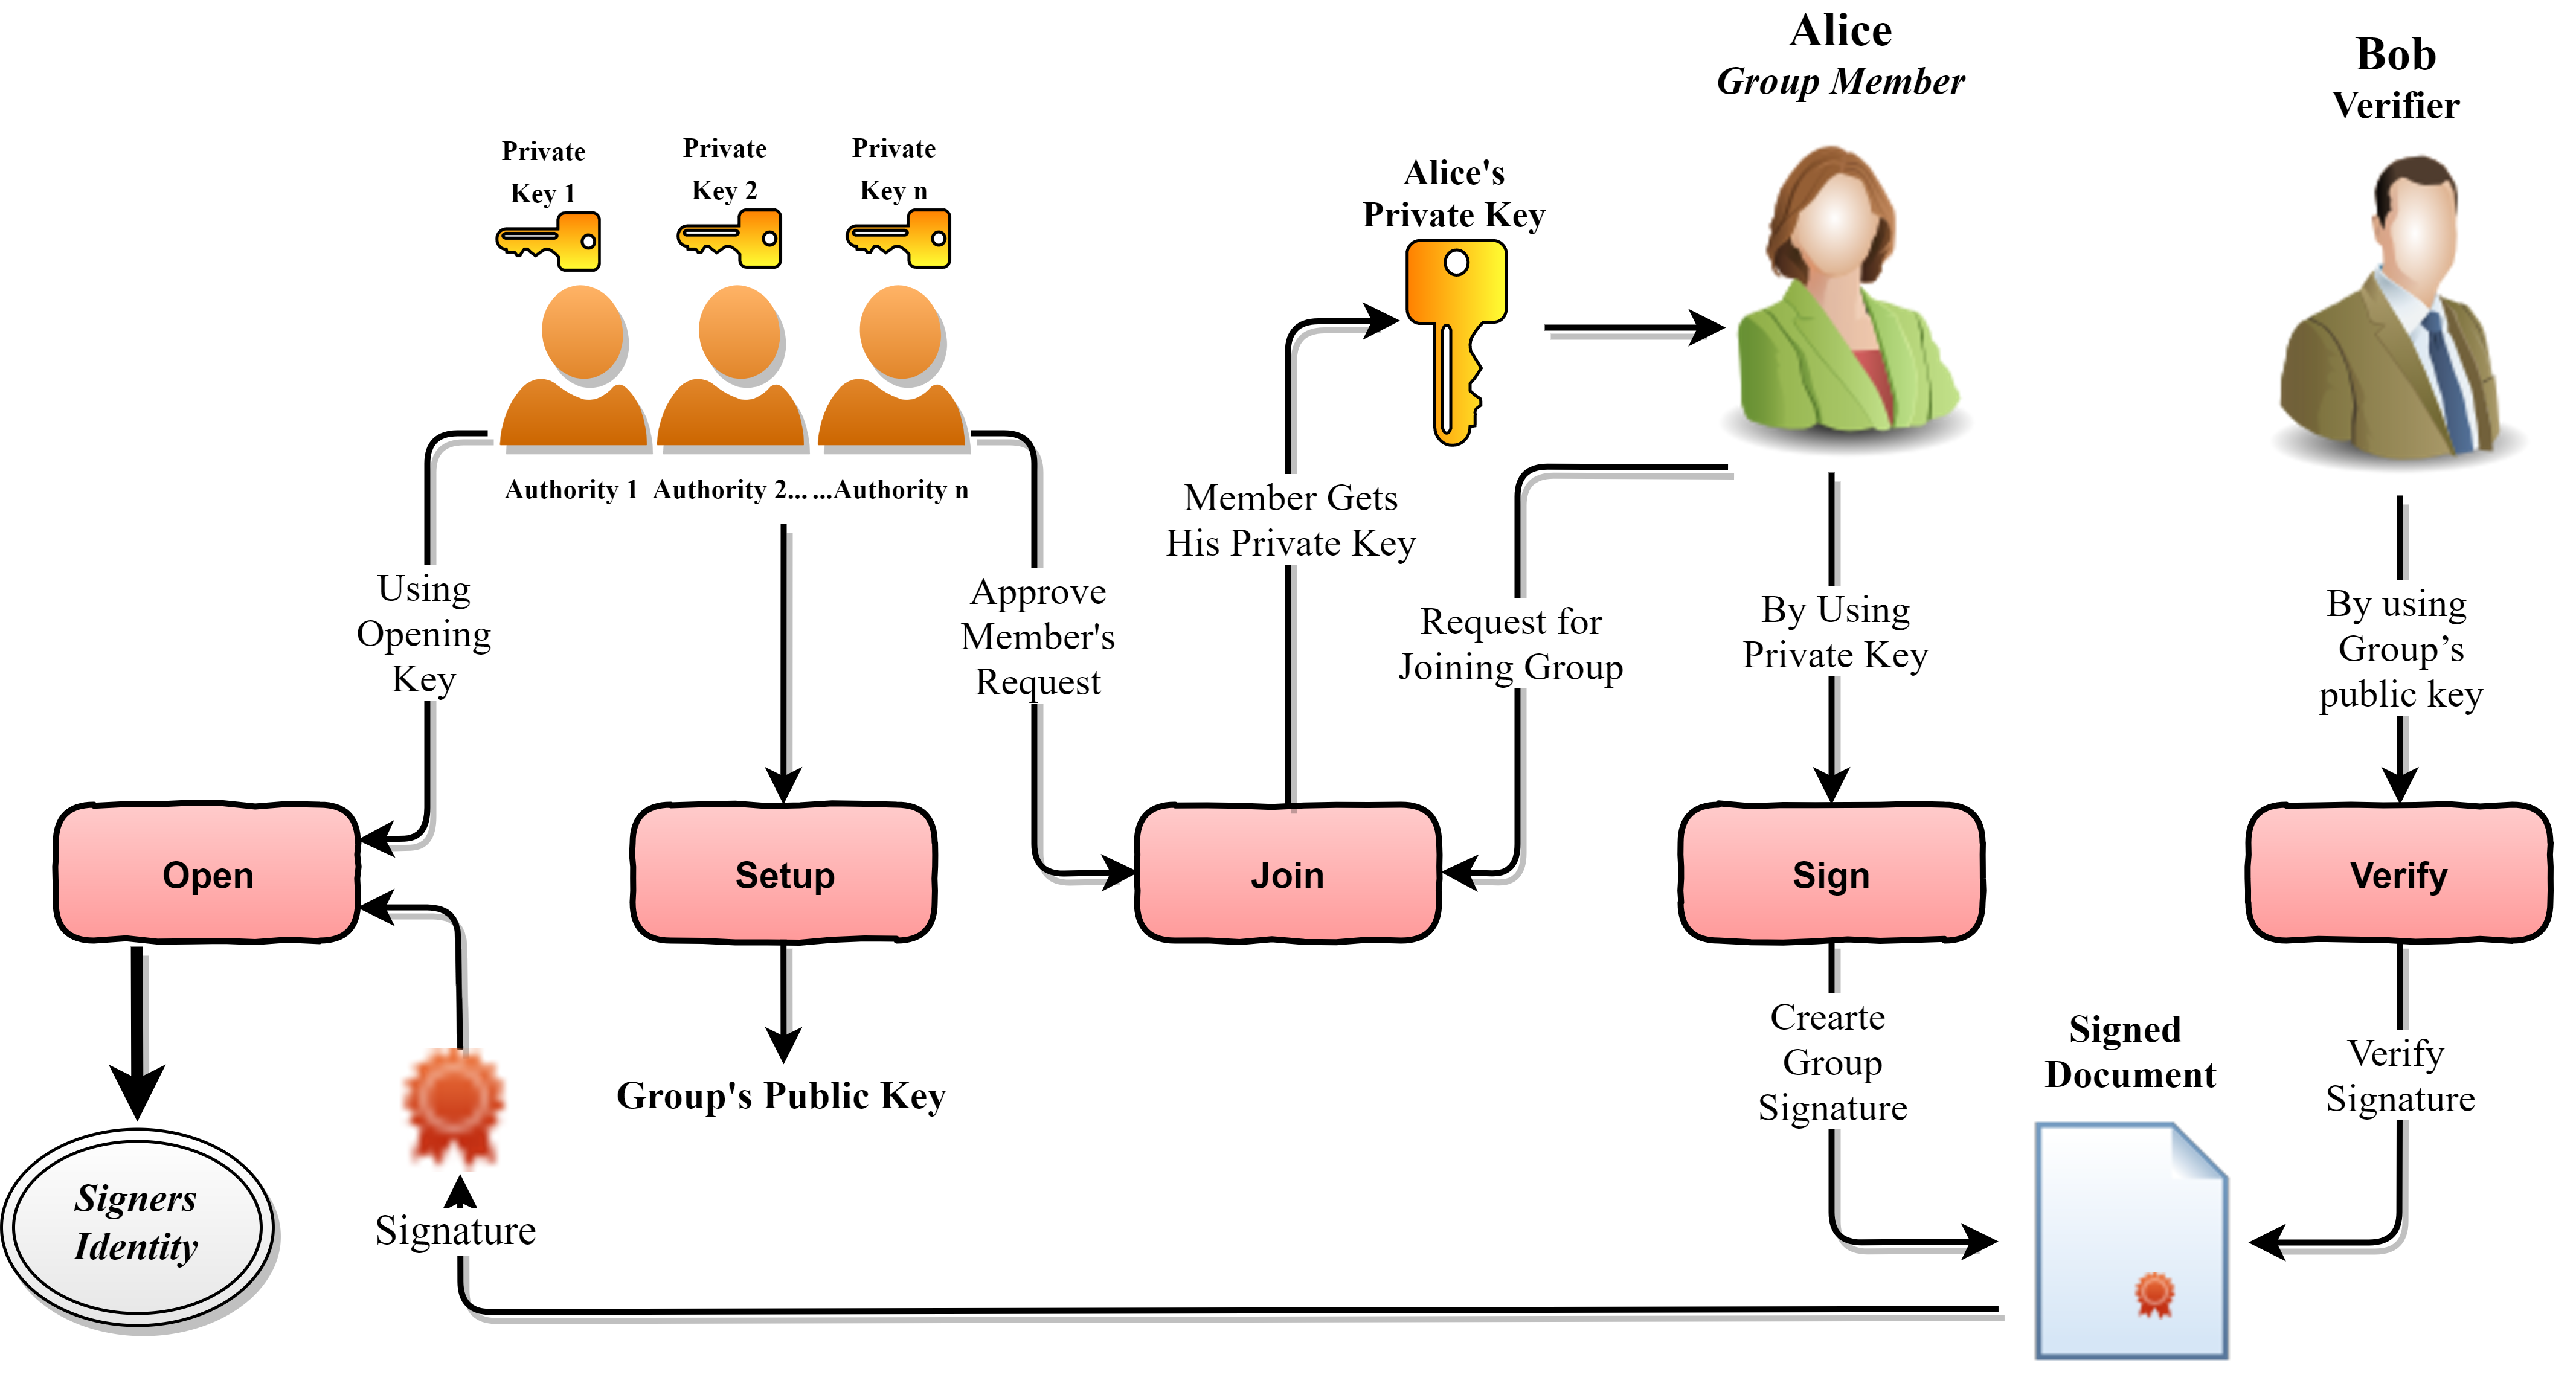
\includegraphics[width=\textwidth]{groupsignaturewithdistributedauthorities}
    \caption{Group Signature Schemes with Distributed Authorities}
    \label{fig:Group Signature Schemes with Distributed Authorities}
\end{figure}
The figure shows architecture of group signature scheme with distributed authorities. In the figure, various authorities are shown that are responsible for different tasks. One authority is responsible for generating the public key of the group, another authority is responsible for joining the members in the group, and the role of the opening signature is assigned to separate authority. Each authority in the figure is in possession of the different private key. The role of signer and verifier are similar to that of other group signatures schemes.

\subsection{Group Signatures with Unique Properties}\label{subsection:GSUniqueProperties}
Although the classification of the group signatures in the earlier section covers most of the group signatures schemes, some schemes are not included in it. Those schemes have a unique construction whose properties are not comparable with most of the common group signature schemes.
\subsubsection{Blind Group Signature}
A Blind group signature\index{blind group signature} scheme is a combination of blind signatures and group signatures. The blind group signature work in the following manner. A group signature is generated in such a way that signer should not be able to see the message $M$, which chosen by a third party. The third party also does not know the identification of the signer. After concluding this interaction, the third party gets a valid group signature for the message $M$, and signer doesn't have any knowledge of the message or the signature produced by his private key.

Lysyanskaya proposes the application of this fascinating structure\cite{lysyanskaya1998group}. The purpose of the application of blind group signatures is that the signature generation process should be unlinkable to the message as well as the signature. Application of Lysyanskaya describes an electronic cash system in which issuer bank is the blind signer, and the signed message can be considered as an electronic currency. As a part of a financial group, the issuer bank provides the electronic money to a customer at the time of withdrawal, and the customer can use this currency for transactions without revealing any information about the issuer bank as well as disabling the issuer bank to track the utilization of this electronic currency by the client.

\subsubsection{Democratic Group Signature}
The mathematical structure of Democratic group signature\index{democratic group signature} is built in such a way that the need for authorities, especially the Group Manager is eliminated\cite{manulis2006democratic}\cite{manulis2006linkable}. Instead, the tasks of Group Manager are executed by the group members. The group members can work democratically because the scheme provides such a unique power to all the group members. The addition and revocation of the members are done jointly, where members are required to agree in a majority. The opening of the signature is done by each member individually. Here each member has the ability to link any signature to its original signer. The verifier, who are not group members are still unable to link the signature to its original signer, and signatures remain anonymous to the verifiers. 

Some democratic group signature scheme can restrict the opening ability to a limited subset of group members\cite{li2009}. Some schemes allow the signer to decide such subset of members having the opening ability\cite{li2009democratic}. In those schemes, each subset of members can open specific signatures but not all the signatures.

\subsubsection{Mediated Group Signature}
In the Mediated group signature\index{mediated group signature} scheme an additional entity named the Mediated Server is present\cite{ding2004leak}. This entity is required for generation of the signatures by group members. For generating a signature a signer required to identify themselves to the Mediator server and provide a partial signature. After getting the partial signature, the mediating entity is able to generate full group signature if the signer is not revoked. The mediation entity is also useful in the revocation of the members. The mediated entity maintains a list of revoked members and adds a member in the list on the request of the Group Manager. The mediated group signature has a unique security property known as leak-freedom. The leak-freedom property prevents the group members from producing past signed signatures.

\section[Group Signature Schemes based on General Assumptions]{Group Signature Schemes based on \\General Assumptions}
To implement the group signature scheme some authors proposed a different way which was based on generic solutions and uses cryptographic primitives in a black box way. Which means in simple terms the scheme is constructed using the schemes and algorithms which were already devised and used for different purposes. Although these type of systems are found to be less efficient than the schemes based on number theoretical assumptions, they provide the need of hardness assumption to prove security and also elaborate some design specifications required for security of the group signature schemes. Following section represent some notable group signature schemes which are based on general assumptions. These schemes use the \textquotedblleft sign and encrypt and prove\textquotedblright ~ pattern which is also employed in some other group signatures.

\subsection{The Bellare Micciancio Warinschi Scheme}
The construction of The Bellare Micciancio Warinschi Scheme\index{Bellare Micciancio Warinschi Scheme} (hereinafter referred as the BMW scheme) is based on digital signature scheme, asymmetric key encryption and noninteractive zero-knowledge protocol for proof of knowledge\cite{bellare2003foundations}. The BMW scheme builds on the generic scheme proposed by Camenisch and Michels\cite{camenisch1999separability}. 

The generic algorithms in cryptography used by the BMW scheme are:
\begin{itemize}
\item A digital signature scheme $DS$ = (Key Generation, Sign, Verify).
\item An asymmetric encryption scheme $PKE$ = (Key Generation, Encrypt, Decrypt).
\item A noninteractive zero-knowledge protocol for zero knowledge proof.
\end{itemize}

In the BMW scheme, the private key of a member $i$ is made up of a secret key $sk_i$ and a Digital Certificate $Cert_i$, which was issued by the Group Manager. Therefore the certificate can be viewed as the certificate of Group Manager on member's public key. To generate a signature for a message $M$, the member $i$  encrypts $(i, pk_i, Cert_i)$ by using the public key of the group $gpk$. Then the member generates digital signature $S$ by using $sk_i$ on message $M$ and provide a proof of knowledge by the noninteractive zero-knowledge protocol. For verification of the signature $S$, a verifier provides an input of $gpk$, message $M$ and signature $S$ to the \texttt{Verify} algorithm, which parses the signature $S$ and validate the zero knowledge proof given by the signer in the signature. To associate a signature to its signer, the Group Manager decrypts the $(i, pk_i, Cert_i)$ by using $gsk$ and find out the identity of the signer using $cert_i$. 

The BMW scheme does not support verifiable opening and accusation a member by Group Manager is possible. The zero-knowledge proof provided by the group member can be extended in such a way that accusation of members should not be possible. The BMW scheme is a static group signature scheme and does not support the addition of any new members after the commencement of the group, but the revocation of any member can be done by making some modifications in the scheme. By default, the proposed scheme does not have any member revocation mechanism in it. The BMW scheme provides various security properties like nonframeability and traceability. The scheme also satisfies full anonymity defined in \cite{bellare2003foundations} called as Beller's model of Group Signature. The modified adaptation of this system which supports the addition of members after the creation of the group and enhanced security is explained in the next section.

\subsection{The Bellare Shi Zhang Scheme}
The Bellare Shi Zhang scheme\index{Bellare Shi Zhang scheme} is a dynamic group signature scheme created using generic algorithms\cite{bellare2005foundations}. The scheme not only provides a verifiable opening but also distributes the task of Group Manager into two separate authorities. One authority is responsible for issuing the $mpk$ and joining the members who called the \texttt{Issuer} and another authority responsible for associating the signature to its original signer named as the \texttt{Opener}. The scheme also implements a system of user PKI for possible members. The Bellare Shi Zhang scheme is very much similar to the static BMW scheme and uses a unforgeable digital signature scheme, an asymmetric encryption algorithm and two noninteractive zero-knowledge protocol for zero knowledge proofs. 

The \texttt{SetUp} algorithm of the Bellare Shi Zhang scheme uses both the digital signature scheme and asymmetric encryption scheme to generate private keys of the \texttt{Issuer} and the \texttt{Opener} in the following fashion. First, two common reference strings are calculated by taking an input of parameter $1^k, k \in \mathbb{N}$. Then a public and private key pair is generated for the digital signature scheme, and another public and private key pair is generated for the asymmetric encryption algorithm. The public key of the group is a tuple of the two common reference strings and both public keys of digital signature and asymmetric encryption algorithm. The private key of the \texttt{Issuer} is the private key of the digital signature scheme, and the private key of the \texttt{Opener} is the private key of the asymmetric encryption algorithm. The \texttt{SetUp} algorithm also generates a $List$ of users which is empty at the beginning. 

The \texttt{Join} protocol of the scheme is required to be executed in a secure channel because of the transmission of the private key and $cert_i$ of the member. In this system, the user generates his own private and public key pair for the digital signature scheme and get $cert_i$ from the \texttt{Issuer}, and the public key of the user is stored in the $List$.

The signature generation and signature verification procedure are exactly same as the BMW scheme which is discussed in the previous section. Whereas, the \texttt{Open} algorithm is also similar to the BMW system, except the addition of the signer's identity and the requirement of a separate private key of the \texttt{Opener} for opening the signature. The \texttt{Open} algorithm of this scheme also provides a publicly verifiable proof of the opened signatures which can be verified by using the \texttt{Judge} algorithm. Revocation mechanism is not provided in the proposed scheme, but an extension is possible
%by various mechanisms like verifier-local revocation 
to allow revocation.
% of a member. 

The security of the Bellare Shi Zhang scheme is similar to that of the BMW scheme and provides full anonymity, traceability, and nonframeability. The nonframeability is the additional security property present in this scheme than the BMW scheme.

\section[Group Signature Schemes using RSA assumption]{Group Signature Schemes using\\ RSA assumption}
\index{group signature schemes using RSA assumption}The RSA\nomenclature{RSA}{Rivest, Shamir, and Adleman algorithm for asymetric cryptography} assumption is found to be useful not only for the digital signatures schemes but also for the group signature schemes. An earlier scheme, which uses the RSA assumption, was proposed by D. Chaum\cite{chaum1991group}. This proposed scheme had some shortcomings in it like the security requirements were not entirely satisfied as of modern needs. Also in that scheme, the length of the group public key and the signature was quite long. The scheme was a static signature scheme and does not support the later addition of members in the group. A dynamic scheme, which is based on the RSA assumption was proposed by Camenisch and Stadler\cite{camenisch1997efficient}. Their scheme produces a uniform length of signature and group keys. The scheme of Antenies and Tsudik offers a more efficient variant with dynamic group signatures\cite{ateniese1999group}. Whereas, the scheme proposed by Camenisch and Michels was also efficient static group signature with a verifiable opening algorithm\cite{camenisch1998group}. All these schemes use the RSA assumption as a base for their security. 

None of the schemes mentioned above offers revocation of a member from the group, but several extensions were offered to deal with this shortcoming. The article of Bresson and Stern proposes a modification of the Camenisch and Stadler scheme\cite{camenisch1997efficient} to enable revocation of group members\cite{bresson2001efficient}. The extension of Ateniese et. al. \cite{ateniese2002quasi} uses noninteractive zero-knowledge proofs for revocation procedure in the ACJT scheme. Camenisch and Lysyanskaya proposed an out of the box solution of using dynamic accumulators for the purpose of revocation of members in the group signature scheme\cite{camenisch2002dynamic}. 

The group signature scheme of Nakanishi and Sugiyama was a dynamic group signature scheme with distributed authorities\cite{nakanishi2004group}. An amendment of this scheme was also proposed by Nakanishi for efficient update of members private key for unrevoked group members but increases the load of Group Manager\cite{nakanishi2005group}. The paper of Camenisch and Groth proposes multiple group signature schemes based on RSA assumption\cite{camenisch2004group}. These schemes were static and dynamic in nature and support revocation of members. The next section provides a detailed discussion about some important group signature schemes which are based on the RSA assumption.

\subsection{The ACJT Scheme}\label{ACJT}
This section elaborates the group signature scheme introduced by Ateniese, Camenisch, Joye, and Tsudik\cite{ateniese2000practical}. This scheme is a dynamic group signature scheme and popularly known as the ACJT scheme\index{ACJT scheme}. This scheme has been adapted from numerous schemes like the Camenisch and Stadler scheme\cite{camenisch1997efficient}, Camenisch and Michel scheme\cite{camenisch1998group} and Ateniese and Tsudik scheme\cite{ateniese1999group} which were discussed in the previous section. 

The unique advantage of the ACJT scheme is that the practical implementation of the scheme was possible. The scheme provides a verifiable opening procedure and has the ability to generate group public and private keys along with the signature with uniform length. The scheme was also resistant to the coalition of members attack, which is an essential security requirement for a group signature scheme. The security of the scheme was not only dependent on the RSA assumption but also the quadratic reciprocity assumption and Diffie-Hellman assumption were used to enhance the security. The scheme was able to implement almost all the modern security properties required for a group signature scheme and mathematical proofs of that are also provided for them. 

The scheme defines a set of security parameters $\lambda_2, \lambda_1, \gamma_2, \gamma_1$ and ranges $\Gamma, \Lambda$ in the following way.
\[
\lambda_2 \geq 4\ell_p, 
\lambda_1 \geq \varepsilon(\lambda_2 + k) + 2 , 
\gamma_2 \geq \lambda_1 + 2 , 
\gamma_1 \geq \varepsilon(\gamma_2 + k)+ 2 ,
\]
\begin{center}
and ranges $\Gamma = ]2^{\gamma_1-\gamma_2}, 2^{\gamma_1+\gamma_2}[$ and 
		   $\Lambda = ]2^{\lambda_1-\lambda_2}, 2^{\lambda_1+\lambda_2}[$.
\end{center}

\subsubsection{SetUp}
The \texttt{SetUp} algorithm of the ACJT scheme uses two large prime numbers $p^\prime$ and $q^\prime$ in the strong RSA assumption and calculate the RSA modulus as $n = (2p^\prime + 1)(2q^\prime + 1)$. The public and private keys of the group are generated in the following manner.

\begin{algorithm}
\caption{\texttt{SETUP} of ACJT scheme}
\begin{algorithmic}[1]
\STATE Generate random numbers $g, h, a, a_0 \in \operatorname{QR}(n)$ and of order $p^\prime q^\prime$.
\STATE Select random $x$ and calculate $y = g^x (mod~n)$
\STATE Group Manager sets group's public key as \framebox[1.1\width]{$\mathcal{Y} = (n, a, a_0, y, g, h)$}.
\STATE Group Manager sets group's private key as \framebox[1.1\width]{$\mathcal{S} = (p^\prime, q^\prime, x)$}.
\end{algorithmic}
\end{algorithm}

In the \texttt{SetUp} phase, the RSA modulus is assumed to be safe and in possession of a trusted party. The public key elements $(g, h, a, a0)$ selected randomly from $QR(n)$.

\subsubsection{Join}
The \texttt{Join} algorithm is a protocol between Group Manager and a user, resulting the user becoming a member of the group by getting his private key. The \texttt{Join} algorithm of the ACJT scheme is more secure than previous schemes and uses zero-knowledge proof. The procedure of the \texttt{Join} algorithm is as follows.

\begin{algorithm}
\caption{\texttt{JOIN} protocol of ACJT scheme}
\begin{algorithmic}[1]
\STATE User $U_i$ generate random exponent $\hat{x}_i \in_R ]2, 2^{\lambda_2}[$ and random number $\hat{r} \in_R ]0, n^2[$ then send $C_1 = g^{\hat{x}_i}h^{\hat{r}}(mod~n)$ to Group Manager. also proves his knowledge of $C_1$.
\STATE Group Manager verifies $C_1 \in \operatorname{QR}(n)$, if verified, then selects $\alpha_i$ and $\beta_i$ $\in_R ]2, 2^{\lambda_2}[$ and sends $\alpha_i$ and $\beta_i$ to user $U_i$.
\STATE User $U_i$ computes $x_i = ( \alpha_i \hat{x}_i + \beta_i (mod~2^{\lambda_2})) + 2^{\lambda_1} $ and sends $C_2 = a^{x_i}(mod~n)$. User $U_i$ also provide zero-knowledge proof for $C_2$.
\STATE Group Manager checks $C_2 \in \operatorname{QR}(n)$. If it is, then selects a random prime $E_i \in_R \Gamma$ and calculate
\framebox[1.1\width]{$A_i = (C_2 a_0)^{E_i^{-1}} (mod~n)$}
and send $U_i$ membership certificate $[A_i, E_i]$
\STATE User $U_i$ verifies if $a_0 a^{x_i} = A_i^{E_i} (mod~n)$.
\end{algorithmic}
\end{algorithm}

\subsubsection{Sign}
To generate a signature for a message, the user required his private key and group public key. The method of generating a signature is as follows.
\begin{algorithm}
\caption{\texttt{SIGN} algorithm of ACJT scheme}
\begin{algorithmic}[1]
\STATE Signer generate random number $w \in_R \{ 0,1 \}^{2\ell_P}$ and calculate 
$T_1 = A_i y^w (mod~n)$,
$T_2 = g^w (mod~n)$,
$T_3 = g^{e_i}h^w(mod~n)$.
\STATE Generate random number
$r_1 \in_R \pm \{ 0,1 \}^{\varepsilon(\gamma_2 + k)}$, 
$r_2 \in_R \pm \{ 0,1 \}^{\varepsilon(\lambda_2 + k)}$, 
$r_3 \in_R \pm \{ 0,1 \}^{\varepsilon(\lambda_1 + 2\ell_p + k + 1)}$,
$r_4 \in_R \pm \{ 0,1 \}^{\varepsilon(2\ell_p + k)}$.
and calculate
$d_1 = T_1^{r_1} / a^{r_2}y^{r_3} (mod~n)$,
$d_2 = T_2^{r_1} / g^{r_3} (mod~n)$,
$d_3 = g^{r_4} (mod~n)$,
$d_4 = g^{r_1}h^{r_4}(mod~n)$.\\

\framebox[1.1\width]{$C = \mathcal{H}(g\parallel h\parallel y\parallel a_0 \parallel a\parallel T_1\parallel T_2\parallel T_3\parallel d_1\parallel d_2\parallel d_3\parallel d_4\parallel M)$}.\\

$s_1 = r_1 - C(E_i- 2^{\gamma_1})$,
$s_2 = r_2 - C(x_i- 2^{\lambda_1})$,
$s_3 = r_3 - C E_i w$,
$s_4 = r_4 - C w$. in $\mathbb{Z}_n^*.$

\STATE Output \framebox[1.1\width]{$(C, s_1, s_2, s_3, T_1, T_2, T_3)$}.
\end{algorithmic}
\end{algorithm}

Note that a separate ElGamal encryption\cite{elgamal1985public} is required to generate the $T1$ and $T2$.

\subsubsection{Verify}
To verify a signature, verifier required the public key of the group along with the signature and the message. The verifier verifies the signature in the following manner.
\begin{algorithm}
\caption{\texttt{VERIFY} algorithm of ACJT scheme}
\begin{algorithmic}[1]
\STATE Calculate $C^\prime = \mathcal{H}(g\parallel h\parallel y\parallel a_0\parallel a\parallel T_1\parallel T_2\parallel T_3\parallel
\frac{(a_0^C T_1^{s_1-C2^{\gamma_1}})} {(a^{s_2-C2^{\lambda_1}}y^{s_3})}
\parallel \frac{(T_2^{s_1- C2^{\gamma_1}})}{g^{s_3}}
\parallel T_2^C g^{s_4}
\parallel (T_3^C g^{s_1-C2^{\gamma_1}} h^{s_4}
\parallel M) $.
\STATE Signature is valid if and only if $C = C^\prime$ and 
$s_1 \in \{ 0, 1\}^{\varepsilon(k + \gamma_2)+1}$,
$s_2 \in \{ 0, 1\}^{\varepsilon(k + \lambda_2)+1}$,
$s_3 \in \{ 0, 1\}^{\varepsilon(k + \lambda_1+2\ell_p + 1)+1}$,
$s_4 \in \{ 0, 1\}^{\varepsilon(k + 2\ell_p) + 1}$.
\end{algorithmic}
\end{algorithm}

\subsubsection{Open}
To associate a signature to its original signer, the Group Manager performs the following procedure using his private key.
\begin{algorithm}
\caption{\texttt{OPEN} algorithm of ACJT scheme}
\begin{algorithmic}[1]
\STATE Verify the validity of signature by \texttt{VERIFY} algorithm.
\STATE Calculate $A_i$ (The identity of $U_i$) as \framebox[1.1\width]{$A_i = T_1/T_2^x$}.
\STATE Provide Proof that $\log_g y = \log_{T_2}{T_1 / A_i}$.
\end{algorithmic}
\end{algorithm}

The \texttt{Open} algorithm of this scheme also provides a noninteractive zero-knowledge proof to avoid framing of a member by the Group Manager.

\subsubsection{Security of the ACJT scheme}
The ACJT scheme is a Pioneer in providing a most secure scheme with mathematical proofs that why this scheme is considered to be \textquotedblleft state of the art\textquotedblright. The scheme provides full anonymity as defined in Bellare strict model\cite{bellare2003foundations}. The scheme also found to be providing unforgeability, unlinkability, exculpability along with traceability and resistance to coalition.

\subsection{The Tsudik and Xu Scheme}\label{TX}
A dynamic variant of the ACJT scheme allowing revocation of members was suggested by Tsudik and Xu\cite{tsudik2003accumulating}\index{Tsudik and Xu scheme}. In this scheme the dynamic accumulator is formed by $n = n_1 * n_2$,  where $n_1$ and $n_2$ are big prime numbers and kept secret similar to the RSA modulus. The Tsudik and Xu scheme enable their group members to generate their own $n_i$ at the time of joining procedure, and the $n_i$ is placed in the accumulator by the Group Manager as a part of group public key. Group members use the knowledge of factorization of $n = n_1 * n_2$ to generate a signature for a message. The key generation mechanism of the Tsudik and Xu scheme is similar to ACJT scheme except the generation of dynamic accumulators at the commencement of the group. The public key and private key of the group are also very much similar to that of ACJT scheme. In the \texttt{Join} algorithm of this scheme, the user computes $n_i = n_1 * n_2$ and sends $n$ to the Group Manager. The Group Manager then adds the $n_i$ in accumulator after verifying it and sends user $acc_i$.

An important vulnerability of the scheme is that the accumulator is made up of composite numbers $n_i = n_{1i} * n_{2i}$, $n_j = n_{1j} * n_{2j}$ so a colluding attack it possible for members $i$ and $j$ because they can form some another values like $n_{1i} * n_{1j}$ , $n_{2i} * n_{2j}$ and forge a membership certificate that results into inadequate traceability. The \texttt{Sign} algorithm of this scheme is pretty much similar to the ACJT scheme except the use of accumulator in the signature generation and requirement of $T4$ and $T5$ values in the signature which apparently increases the size and cost of generation of the signature. The \texttt{Verify} algorithm and \texttt{Open} algorithm are also similar to ACJT scheme with slight modifications. The important contribution of the Tsudik and Xu scheme is the revocation mechanism which is done by updating the accumulator $acc_i$ in group public key as the $acc^{n_{i}^{-1} (mod~4 p\prime q\prime)} mod~N$ and replacing the entry of $n_i$ with \texttt{del}.

Apart from the security flaw mentioned earlier, the Tsudik and Xu scheme offers various security properties like nonframeability, unlinkability, and exculpability. The anonymity provided by this scheme is not full anonymity according to the  Bellare's model but partial anonymity (or simply anonymity). Similarly, full traceability is not offered by the scheme instead, only insider traceability is provided.

\subsection{The Camenisch and Groth Scheme}\label{CG}
The Camenisch and Groth scheme\index{Camenisch and Groth scheme} is a static group signature scheme which utilizes the RSA assumption\cite{camenisch2004group}. The Camenisch and Groth scheme is slightly faster than the ACJT scheme because of the modified Join algorithm. The basic scheme required a predefined number of group members to produce their private keys, and the Group Manager is an authority trusted to create and distribute private keys of the members. All the algorithms in this scheme similar to the Camenisch and Lysyanskaya scheme\cite{camenisch2002dynamic}. The original Camenisch and Groth scheme provides full anonymity and full traceability as well as nonframeability. The static nature of the scheme results in the limitation of some functionalities like the addition of new members is not possible also revocation of members is not described in the scheme. 

But to overcome these shortcomings, several modifications were recommended. The extension proposed by The Camenisch and Groth enables the later addition of members into the group, converting it to a dynamic group signature scheme. An algorithm for revocation of the members was also introduced which was similar to Camenisch and Lysyanskaya scheme's revocation algorithm where dynamic accumulators are used for the purpose of the revocation\cite{camenisch2002dynamic}. 

A separate extension was also introduced which incapacitates members from generating a valid signature from an old public key. This problem was addressed by combining the accumulator based approach with the local verification revocation approach. Those extensions provided not only same security properties as of the static version of the scheme but also offers full revocability and a verifiable opening of signatures.

\subsection{The Kiayias and Yung Scheme}\label{KY}
In this section, we are going to describe the scheme proposed by Kiayias and Yung\index{Kiayias and Yung Scheme}\cite{kiayias2005efficient}\cite{kiayias2006secure}. This scheme is not only a simple dynamic group signature scheme but also provides a verifiable opening procedure in it. The Kiayias and Yung scheme can be seen as the modification of ACJT scheme where RSA assumption is the base of the security. The setup algorithm of this scheme is almost same as the ACJT scheme except for the requirement of additional $\hat{y}$ and $\hat{x}$ in group public key and private key.

The \texttt{Join} algorithm of the scheme required the support of a third party to add a new member to the group. Also, it separates the member certificates from members private keys. In the \texttt{Sign} algorithm, new element $T_5$ was introduced and required two pairs of ElGamal encryption whereas in ACJT scheme only one pair was needed. The \texttt{Verify} and \texttt{Open} algorithms are similar to the ACJT scheme. 

The Kiayias and Yung scheme offers various security properties like full anonymity, full traceability, and nonframeability. But the extended length of the signature and number of elements in the key results in increased burden of computation to all members including Group Manager. The revocation of the members was not discussing this scheme, so no approach is available to enable the revocation of the members. To enable the distributed authorities the scheme divides the private key elements into two different authorities viz. \texttt{Issuer} and \texttt{Opener}.

\section[Group Signature Scheme using Discrete Logarithms]{Group Signature Scheme using \\ Discrete Logarithms}
\index{group signature using discrete logarithms}Although some group signature schemes use the discrete logarithm setting for their security, it appears that the discrete logarithm technique is not a very attractive setting for group signature schemes. In the discrete logarithms, group signature schemes are less efficient than the RSA schemes. Also, pure discrete logarithms are unable to implement the permutation trapdoor which is essential for the modern security of group signatures. Hence, most of the schemes in this domain uses a mixed setting where the use of RSA assumption is employed for additional security. 

The first scheme which uses discrete logarithm was proposed by Chen and Pedersen\cite{chen1994new}. Although, their scheme was dynamic in nature but can be considered as efficient. The length of generated signature was not fixed, and the security properties of this scheme were not sufficient like the scheme was vulnerable to coalition attack. Also associating a signature to its original signer required all the group members to cooperate with Group Manager. The scheme of Petersen also shows similar drawback as mentioned earlier\cite{petersen1998convert}. The following section provides a discussion of some notable group signature schemes which use the discrete logarithm setting for their security.

\subsection{The Ateniese de Medeiros Scheme}\label{AM}
A notable group signature scheme which uses dynamic logarithm setting was proposed by Ateniese and Medeiros\cite{ateniese2003efficient}\index{Ateniese de Medeiros Scheme}. The scheme allows verifiable opening of the signatures and dynamic addition of the group members. This scheme required a PKI system to distribute certificates to group members. The \texttt{SetUp} algorithm of this scheme required three security parameters and a trusted third party is assumed to be storing the strong RSA modulus. In the \texttt{SetUp} procedure of this scheme the parameters are calculated by determining a strong RSA modulus $\bar{P}$ where $\bar{P}= 2P + 1$ and $P= 2Q + 1$  and all $\bar{P}, P, Q$ are prime numbers. This secure RSA modulus is kept secure, and the parameters can be shared by multiple groups as long as the factorization of the modulus is not revealed. The \texttt{Join} algorithm of the scheme is a type of Nybra Rueppel Signature\cite{nyberg1996message} modified for using the public key of the group. 

The \texttt{Join} algorithm is required to be executed in a secure manner of communication so no intruder can identify the private key of the members. The signature is generated by this private key of the member, and two separate ElGamal encryptions are required for the signature elements similar to ACJT signature. The length of the signature depends on the length of the hash function used for the message. The verification of the signature is done by validating the proof of knowledge provided by the signer. 

The opening procedure is also a remarkably similar to the ACJT scheme where identification of the signer is generated by using $T_1$ and $T_2$ along with the private key of the group. The \texttt{Open} algorithm also produces a proof of knowledge for public verification. The scheme does not provide any security proof in \cite{ateniese2003efficient} except for the claim that the scheme is secure under random oracle model. This scheme provides anonymity but not full anonymity and traceability, and the proof of opening signature prevents framing attacks.

\subsection{The Furukawa Yonezawa Scheme}\label{FY}
The Scheme proposed by Furukawa and Yonezawa\index{Furukawa Yonezawa Scheme} is dynamic group signature scheme with distributed authorities\cite{furukawa2004group}. The scheme uses discrete logarithm assumption for its implementation and security. This scheme also provides a verifiable opening which provides a proof of correctly opened signatures by the Group Manager. This scheme also required a PKI system for key management. 

The key generation required a single parameter and strong RSA modulus which is assumed to be safe by a trusted third party. The \texttt{Join} protocol of this scheme is similar to the Ateniese de Medeiros Scheme and uses an adaptation of Nybra Rueppel Signature under Group Manager or in this case the \texttt{Issuer} of the public key. The \texttt{Sign}, \texttt{Verify} and \texttt{Open} algorithms are not very much different from the Ateniese de Medeiros Scheme and the ACJT scheme. 

Furukawa and Yonezawa provide various proofs and security of their scheme. The security properties of the scheme are traceability, full anonymity, and nonframeability. The scheme also provides an interesting extension in which multiple \texttt{Issuers} and multiple \texttt{Openers} can be implemented by using the threshold secret sharing techniques described by Pedersen in \cite{pedersen1991threshold}. 

\section{Other Notable Group Signature Schemes}
The RSA and discrete logarithms assumptions are not the only techniques used for implementing group signature schemes. Some remarkable group signature scheme uses different techniques than the technique discussed earlier. Those techniques involve bilinear maps pairing, elliptic curve cryptography, etc. The bilinear pairing maps are considered to be more efficient than the RSA or discrete logarithms to implement group signature schemes. Also, the elliptic curve cryptography which is found to be a more secure approach for public key cryptosystem is also found useful in implementing the group signature scheme. The following section describes some important schemes which use these techniques for their implementation.

\subsection{The Boneh Boyen Shacham Scheme}\label{BBS}
The group signature scheme proposed by Boneh, Boyen and Shacham is a static group signature scheme\index{Boneh Boyen Shacham Scheme} with distributed authorities\cite{boneh2004short}. The distributed authorities are accountable for the task of issuing the private key to the members and associating a signature to its original signer. This scheme is one of the first group signature scheme with uses bilinear pairing in its implementation. The \texttt{SetUp} algorithm of this scheme requires single security parameter and bilinear groups $\mathbb{G}_1 = \langle g_1\rangle$, $\mathbb{G}_2 = \langle g_2\rangle$ and $\mathbb{G}_p$ of prime order $Q$ and a bilinear map $\OE = \mathbb{G}_1 \mathbb{G}_2 \rightarrow \mathbb{G}_p$ and homomorphism $\Psi$ from $\mathbb{G}_2$ to $\mathbb{G}_1$ where $\Psi(g_2) = g_1$.

As the scheme is a static group signature scheme, the \texttt{SetUp} algorithm required  $n$, as a number of group members along with parameter $1^k$ and produces group public key and private key as well as $n$ private keys of the members and registration number for each member. Note that the private key is divided into two separate parts that are \texttt{Issuer's} private key and \texttt{Opener's} private key. The key distribution is required to be performed in a trusted manner as it carries the private key of the members. 

The signer uses his private key and group public key to generate a signature and produce $T_1, T_2, T_3$ as a linear encryption of private key and a signature of knowledge which proves that the signer possesses the private key that can be opened by the opening authority. The verifier uses the proof of knowledge for verification of the signature. The opening entity can associate a signature to its signer but does not provide any proof of knowledge. The scheme provides full anonymity and insider traceability but only provides insider nonframeability and not full nonframeability. 

The paper of Boneh, Boyen, and Shacham also provides an extension which enables revocation of members from the group. This revocation process perhaps reduces the security of the scheme. Another extension of this scheme converts the static scheme into a dynamic scheme and introduces additional \texttt{Join} algorithm for the addition of the members into the group. This extension indeed preserves all the security properties of the original scheme, but revocation of the members is not supported in this extension.

\subsection{The Camenisch Lysyanskaya Scheme}\label{CL}
The scheme proposed by Camenisch and Lysyanskaya\index{Camenisch Lysyanskaya Scheme} was one of the primary group signature scheme constructed by using bilinear maps\cite{camenisch2004signature}. The scheme is dynamic group signature scheme with distributed authorities. The distributed authorities are the \texttt{Issuer} and the \texttt{Opener}. The \texttt{SetUp} of the group is required to be performed in a trusted manner and all the elements required should be chosen at random to guarantee the confidence in the group public key. 

The scheme uses the Cramer Shoup encryption system to generate the private key of the group\cite{cramer1998practical}. The Cramer Shoup cryptosystem is secure under decisional Diffie Hellman assumption. By using the \texttt{Join} algorithm, new members are added to the group. This \texttt{Join} algorithm is needed to be executed in a secure channel to protect the membership certificate from intruders. The Sign algorithm also a derivative of the Cramer Shoup cryptosystem. The proof of knowledge is produced to prove the signer’s knowledge of the private key. The verification is similar to Boneh, Boyen and Shacham scheme and the \texttt{Open} algorithm does not provide any knowledge of proof for Group Manager. Hence the procedure is susceptible to frameability. The scheme provides its security by using Beller’s model and provide full anonymity and insider traceability along with partial traceability. 

\subsection{The Bichsel Camenisch Neven Smart Warinschi Scheme}\label{BCNSW}
The scheme proposed by Bichsel et. al.\index{Bichsel Camenisch Neven Smart Warinschi Scheme} is a dynamic group signature scheme with a verifiable opening\cite{bichsel2010get}. The scheme also requires a user PKI system for members. The attractive feature of this scheme is that it does not follow a typical \textquotedblleft sign encrypt and prove\textquotedblright procedure like other group signature scheme. Also, it provides the shortest signature size and minimum computational time while providing strong security. The PKI of the system uses a unforgeable digital signature scheme. The \texttt{SetUp} of the scheme requires bilinear groups and bilinear maps and two hash functions as random oracles. 

In the key generation process, the PKI system is used to generate the private and public key pair for the group. The \texttt{Open} algorithm takes a linear time according to the number of members. Therefore the Group Manager requires ample resources to open a signature. The \texttt{Open} algorithm also provides a zero knowledge proof for public verification of opening and therefore framing of a member is not possible. The Bichsel et. al. scheme provides security properties like anonymity but not full anonymity and insider traceability and nonframeability. The table \ref{table:variousgroupsignatures} shows different group signatures discussed in this section.
\begin{table}[!h]
\begin{center}
\begin{threeparttable}
\renewcommand{\arraystretch}{1.3}
\caption{Various group signatures schemes.}
\label{table:variousgroupsignatures}
\small
\begin{tabular}{| >{\arraybackslash}m{2.2in} |>{\centering\arraybackslash}m{0.55in} |>{\centering\arraybackslash}m{0.9in} |>{\centering\arraybackslash}m{0.5in} |>{\centering\arraybackslash}m{0.7in} |}
\hline 
\textbf{Group Signature scheme by} & \textbf{Short} & \textbf{Assumption} & \textbf{Section} & \textbf{Refrence}\\ 
\hline\hline
Ateniese Camenisch %
et.al.	 			& ACJT	& RSA & \ref{ACJT}& \cite{ateniese2000practical}  \\ \hline
Tsudik and Xu 		& TX	& RSA & \ref{TX}  & \cite{tsudik2003accumulating} \\ \hline
Camenisch and Groth	& CG	& RSA & \ref{CG}  & \cite{camenisch2004group}\\ \hline
Kiayias and Yung	& KY	& RSA & \ref{KY}  & \cite{kiayias2005efficient}\\ \hline
Ateniese de Medeiros& AM	& DL  & \ref{AM}  & \cite{ateniese2003efficient}\\ \hline
Furukawa Yonezawa	& FY	& DL  & \ref{FY}  & \cite{furukawa2004group}\\ \hline
Boneh Boyen Shacham	& BBS	& BM  & \ref{BBS} & \cite{boneh2004short}\\ \hline
Camenisch Lysyanskaya& CL	& BM  & \ref{CL}  & \cite{camenisch2004signature}\\ \hline
Bichsel Camenisch %
et.al.				& BCNSW	& BM  &\ref{BCNSW}& \cite{bichsel2010get}\\ \hline
\end{tabular}
\end{threeparttable}
\end{center}
\end{table}

\section[Similar Approaches for Authentication with Privacy]{Similar Approaches for Authentication with \\Privacy}
There are some other methods that are proposed to maintain privacy while providing authentication. Although these methods were proposed for different objectives, a lot of them have similar functionality as of the group signatures. That's why these approaches are not group signature, but they are constructed using similar cryptographic foundations as of the group signatures. Also, some strategies of these approaches are similar to group signatures. Following section describe some interesting concepts which are not only analogous to the group signatures but also have similar functionality.

\subsection{Affiliation Hiding Authentication}
The affiliation hiding\index{Affiliation Hiding Authentication} is a protocol composed for implementing authentication while preserving privacy. The concept of affiliation hiding is similar to group signature where it protects members identity by using group based authentication. But the affiliation hiding authentication also masks the identity of the group whereas in group signature authentication the identity of the group is not disguised. The affiliation hiding protocol generally classified into two varieties one is secret handshake protocol, and other is key establishment protocol. The authentication is done by matching the affiliation of both parties in which a viable communication is required. If the affiliation is matched, then the parties become authenticated else protocol gets terminated without providing any knowledge other than the not matching of the affiliation. 

Successful authentication creates a secret key which is used for mutual communication between the authenticated parties. The affiliation hiding protocol has a high potential in shielding privacy while providing authentication in online communication. Another similarity of the affiliation hiding protocol with group signature is that they both have authorities with special powers. These authorities are responsible for independently managing their group. Some affiliation hiding protocol also supports revocation of the members which is usually done by those authorities. The main two kinds of affiliation hiding protocol are linkable and unlinkable affiliation hiding protocols. The linkable protocols are found to be more efficient compared to unlinkable affiliation hiding protocols. The linkable affiliation hiding protocol issues a pseudonym to the user for communication. The pseudonym is made up from the group membership information of the member. The pseudonyms are revocable by the group authorities. To revoke a pseudonym, the group authorities distribute the revocation list to all the members. Some important linkable affiliation hiding protocols are described in \cite{balfanz2003secret, castelluccia2004secret, vergnaud2006rsa, jarecki2008beyond, manulis2011affiliation, manulis2011practical, manulis2010affiliation2}.
 
The unlinkable affiliation hiding protocols employ sophisticated group management methods to prevent any correlation among the session of the same user. The unlinkable protocols are described in \cite{ateniese2007secret, jarecki2007unlinkable, law2009private, tsudik2006flexible}. Some security features are reduced in the unlinkable protocols like in \cite{ateniese2007secret} revocation is not available, in \cite{jarecki2007unlinkable} synchronization of the revocation period is needed between members. Some protocols like \cite{manulis2010affiliation2, manulis2010taming} also shield the identity of the member from the group authorities, so he remains absolutely incognito. Some protocols provide efficient handling of multiple group membership information in a session which increases their practical applicability. The significant difference between affiliation hiding protocol and group signature is that the verifier in the group signature is public whereas, in affiliation hiding protocol, the group members are the one who verifies each other's membership during communication.

\subsection{Anonymous Credential System}
An initial concept of the anonymous credential system\index{Anonymous Credential System} is proposed by Chaum \cite{chaum1983blind} which was a cryptographic system designed to provide authentication while preserving the privacy of the users. Similar to group signature the anonymous credential system user gets their credential certificate from an organization like a group. These credentials provide a unique identification of the user similar to ID cards or other physical paper based credentials like train tickets. The anonymous credential system provides a medium to users by which they can prove their possession of valid credentials without revealing their identity. Primary anonymous credential systems required trusted third parties \cite{chaum1986secure} and not very efficient \cite{chaum1985security, damgaard1988payment, lysyanskaya1999pseudonym}. Advance anonymous credential systems which are designed for security and efficiency were proposed in \cite{camenisch2001efficient, camenisch2002dynamic}. Some more improved version of these systems are \cite{camenisch2004signature, camenisch2008efficient, camenisch2009accumulator, camenisch2010solving}). The system described in \cite{camenisch2009accumulator, camenisch2010solving} also offer revocation of the credentials. The practical approach of the anonymous credential system is discussed by Bichsel et. al. \cite{bichsel2009anonymous} in which such system can be implemented on smart cards. 

The security properties required for the anonymous credential system are unlinkability, unforgeability, and coalition resistance. The revocation of the user is also challenging because of the requirement of preserving privacy. The anonymous credential systems are applied in authentication and access control. The anonymous credentials can be used to prove membership of the user in a particular group which is similar to the concept of group signatures. The important difference between an anonymous credential system and the group signature is that the anonymous credential system cannot identify their user like the \texttt{Open} algorithm in group signatures. The anonymous credential system protects the privacy of the user in this case also.

\subsection{Anonymous Signatures}
The anonymous signatures\index{Anonymous Signatures} are similar to the digital signatures in which private key of the signer is employed to generate the signature, and the public key is applied to verify that signature. This remarkable similarity may question the privacy preserving ability of the anonymous signatures but the anonymous signature work in such a way that message is not publicly disclosed. Yang et. al.  proposes the concept of anonymous signature. al. \cite{yang2006anonymous} where the idea was to provide the message an adequate entropy such that it should withstand the attacks on privacy. 

The paper of Fischlin \cite{fischlin2007anonymous} modified the concept of Yang et. al. and inserted a transformation to add anonymity to a digital signature. The concepts proposed in \cite{bellare2009partial, saraswat2009anonymous, zhang2008strong} divides the digital signature into multiple parts, and at least one part was kept hidden. Anonymous signature provides a different type of anonymity than the group signatures. The Group signature does not fail the anonymity if the pair of message and signature become public whereas in this case, anonymous signatures cannot protect anonymity. Some of the concepts of the anonymous signature are also used in the construction of group signatures.

\subsection{Blind Signatures}
The concept of blind signatures\index{Blind Signatures} was also proposed by Chaum \cite{chaum1983blind} where the signer sign the message without knowing it. The signature is however verified using the public key of the signer. The blind signatures can be imagined like a signer signing a message hidden from him e.g. in a closed envelope. The blind signature system required to entities a user and a signer who is different than the user. The signer signs the message generated by the user. The blind signatures have security properties like unforgeability and unlinkability which protects the privacy of the user. The blind signature has numerous application in electronic cash and similar systems. Apart from the work of Chaum, various blind signature schemes are proposed. The schemes \cite{camenisch2004efficient, kiayias2006concurrent, kiayias2008equivocal} are based on RSA assumption of integer factorization, \cite{pointcheval2000security, abe2001secure, abe2010structure, boldyreva2003threshold} are based on discrete logarithms and bilinear pairings. The concept of the blind signature can be converted into group signatures. The section \ref{subsection:GSUniqueProperties} describes a similar concept in which the blind signatures are modified into group blind signature scheme.

\subsection{Direct Anonymous Attestation (DAA)}
The Direct Anonymous Attestation (DAA)\index{Direct Anonymous Attestation (DAA)}\nomenclature{DAA}{Direct Anonymous Attestation} is a protocol for administering remote attestation to computing platforms without revealing the identity. The remote attestation process requires a tamper proof chip called Trusted Platform Module (TPM)\nomenclature{TPM}{Trusted Platform Module}. The TPM chip is attached to the computing device like smartphones or laptops and contains private key of the issuer. The TPMs are used for authenticating local configuration, and challenge and response protocol implement the process. The TPM chips are found beneficial against impersonation attacks, but the process is required to be shielding privacy. The Brickell, Camenisch, and Chen \cite{brickell2004direct} provides a solution for DAA in which verifier is powerless to extract the private information during attestation. This DAA scheme did not require any trusted third party.

The DAA schemes are similar to group signature. The DAA system is implemented in such a way that throughout attestation process, the verifier is unable to link the TPM to any previous sessions. The primary difference between DAA system and group signature is that the DAA technique cannot identify the TPM in any ways like the opening procedure of the group signature associates the original signer to his signature. No process them to the \texttt{Open} algorithm of group signature is available in the DAA system.

\subsection{Ring Signature}
The ring signatures\index{Ring Signature} are the most similar system described in this section to the group signatures. The ring signature uses the mathematical structure of rings whereas group signatures use the structure of groups. The ring signatures were proposed by Rivest, Shamir, and Tauman \cite{rivest2001leak}. The basic idea behind the ring signature is that a signer is a part of the list contains public key of many users, and when he generates the signature it can only be verified by that list which does not disclose any information about the signer. The ring signatures are unforgeable also because formulating a signature without knowing private key corresponding to the public key in the list is impossible. Also, the ring signature can not be linked to any precise user, so it remains unlinkable. Determining any two signatures are from the same signer or not is not possible in ring signatures. 

The paper of Rivest et. al. describes its application for leaking a secret. Their scheme of ring signature is constructed by employing trapdoor permutation. The idea of \cite{rivest2001leak} was improved by Bender, Katz, and Morselli \cite{bender2009ring} to avoid possible leakage of the private key and insider attacks. The schemes like \cite{liu2004linkable, tsang2004separable, tsang2005short, lee2005convertible, zhang2006new}) offer linkability and verifiability. The linkability property can detect multiple signatures from the same signer, and the verifiability allows the signer to generate a proof of his signature. 

The shortcomings of the ring signatures are the inconsistent length of the signatures and increases linearly. The scheme proposed by Chandran, Groth, and Sahai \cite{chandran2007ring} creates signatures having sub linear to the number of members in the ring. The primary difference between group signature and the ring signature is that the signer in ring signature can use any public key in ring whereas in the group signature signer needs to use his own private key. Also, the opening of the signature is not possible in ring signature scheme, so the anonymity of the signer remains unconditional.

\subsection{Traceable Signature}
The traceable signatures\index{Ring Signature} are different types of the group signature in which traceability is redefined differently than the group signatures. The fundamental concept of the traceable signature is introduced by Kiayias, Tsiounis, and Yang \cite{kiayias2004traceable}. In the traceable signature, the Group Manager have special tracing trapdoor for every member. The tracking agents can identify all the signatures issued by a member if the trapdoor is revealed by the Group Manager. Therefore the traceable signature offers anonymity and unlinkability but the revocation and opening of the signature is the same process in it. 

The opening of a single signature is not possible in the traceable signature. Also once the trapdoor is public, the user cannot sign anonymously. But in the group signature opening a single signature does not associate another signature of same signer and revocation is different than that traceable signatures. Also in the traceable signature, the signer can claim a signature later, but the group signatures do not offer such functionality.

\section{Cryptographic Foundations}
The modern cryptography relies on various number theory principles and assumptions. The group signature scheme is also constructed using these principles. This section provides a brief discussion about some basic cryptographic principles and foundations. These principles are also used in the construction of proposed group signature scheme. Some of the assumptions discussed in this section are providing a base to many modern cryptographic techniques and schemes. The following discussion introduces some basic foundations and assumptions on which the proposed group signature is depended and the security of the scheme is assumed.

The cryptographic foundations comprise of various primary concepts which are utilized by cryptographic systems. The foundations are the several schemes and methods proposed to solve a particular problem in cryptographic systems. The foundations of cryptography serve as the primary building blocks for different systems. Reliable, secure and robust cryptographic systems can be constructed by using combinations of these components. Some of these foundations are also employed in the construction of group signature schemes. The following section provides a short introduction to these cryptographic foundations.

\subsection{Trapdoor Permutations}\label{sub:Trapdoor Permutations}
This \index{Trapdoor Permutation}section presents definition to the concept of trapdoor permutation. But before that, we need to understand the working of one way functions on which the notion of trapdoor permutation is based.
\subsubsection{One Way Functions}
The one way functions\index{One Way Functions} are constructed in such a way that they are easy to compute but hard to invert. Therefore one way function $f\{0, 1\}^* \mapsto  \{0, 1\}^*$ is constructed using function $f$  which take polynomial time to compute and assume that no polynomial time algorithm is present for reverting the output of function $f$. The formal definition of one way function is as follows.

\begin{definition}[One way function] The function $f\{0, 1\}^* \mapsto  \{0, 1\}^*$ is said to be one way function if it satisfies following two requirements:
\begin{itemize}
\item The function $f$ takes polynomial time and space to produce its output.
\item No polynomial time algorithm is available which can produce the input of function $f$ by taking the output of function $f$.
\end{itemize}
\end{definition}

Like many assumptions in cryptography, the one way function is also an unproven assumption, and there is no proof exists that can prove that the one way function is irreversible. If the length of the output of the one way function $f$ is fixed, then it is called one way permutation.

\subsubsection{Trapdoor Permutation}
The Trapdoor Permutation\index{Trapdoor Permutation} is a function $f\{0, 1\}^* \mapsto  \{0, 1\}^*$ which produces its fixed length output in polynomial time and riveting the output of the function is also takes polynomial time if and only if a secret information is available. This secret information is called the Trapdoor. It is computationally hard to revert a trapdoor permutation to revert without the knowledge of secret information. The formal definition of the Trapdoor permutation is given below.

\begin{definition}[Trapdoor Permutation] A one way permutation $f\{0, 1\}^* \mapsto  \{0, 1\}^*$ with a trapdoor information $\intercal$  is called trapdoor permutation if it follows following three conditions.
\begin{itemize}
\item The function $f$ takes polynomial time and space to produce its output.
\item Reverting algorithm also requires polynomial time when provided with a unique trapdoor information and provides the correct output which is equal to the input of function $f$.
\item No polynomial time algorithm available which can either produce the Trapdoor information from the output of the function $f$ or revert output of the function $f$ without the trapdoor information.
\end{itemize}
\end{definition}

Note that the Trapdoor is not part of the output of function $f$. Therefore it is not possible to produce the Trapdoor information if one knows both the input and output of function $f$. The well known example of the Trapdoor permutation is the RSA cryptosystem in which the factorization of modulus $n$ is the Trapdoor information.

\subsection{Hash Functions}
The Hash function\index{Hash Functions} is a function which accepts an arbitrary length of data and provides a fixed length string called the digest. The hash functions are one way functions which are discussed in the previous section. Because of that, it is computationally hard to revert the hash function and find original data from the digest. As the digest is always of fixed length, the hash functions come into the category of one way permutations. If the digest is of fixed length, then there is always a possibility that there can be two equal digests for different data. This phenomenon is called collision. A secure hash function needs to avoid such collisions. The formal definition of the hash function is given below.

\begin{definition}[Hash Functions] A one way permutation function mapping strings of finite arbitrary length into fixed length string called a Hash Function $\mathcal{H}$.
\[ \mathcal{H}\{0, 1\}^* \mapsto \{0, 1\}^\ell \] 
\end{definition}

\begin{corollary} A hash function is \emph{weak collision resistant} if for a given string $s$ it is computationally hard to find $s^\prime \neq s$ such that $\mathcal{H}(s) = \mathcal{H}(s^\prime)$\cite{naor1989universal}.\end{corollary}

\begin{corollary} A hash function is \emph{strong collision resistant} if it is computationally hard to obtain a pair $(s, s^\prime)$ and $s \neq  s^\prime$ such that $\mathcal{H}(s) = \mathcal{H}(s^\prime)$\cite{damgaard1987collision}.\end{corollary}

From the above corollary, it can be seen that a strong collision resistant function is also a weak collision resistant function.

The hash functions have numerous applications in the field of cryptography. Mostly the hash functions are used for generating Message Authentication Codes (MAC) which are used for checking the integrity of a message. Some hash functions use a secret key along with the one way function while generating the MAC to avoid various attacks, called HMAC. Nowadays passwords are also stored by hashing them so that a data theft should not be able to get the passwords from the database. The hash function is an essential part of digital signatures and also group signatures. The hash functions are used not only to determine the integrity of the message but also for the generation of the signature. The signature uses the hash of the message because of its fixed and short length which reduces a lot of computational efforts while generating the signature. 
\subsection{Random Oracle Model}\label{sub:random oracle model}
Some advanced cryptographic systems like the group signature scheme employ the hash functions. But the security of these schemes is always proved in a model called the Random Oracle Model\index{Random Oracle Model}. The Random Oracle model was proposed by the Bellare and Rogaway \cite{bellare1993random}. The model is based on the assumption on the hash digest. The assumption is that the hashing algorithm alone cannot generate the digest, but it requires assistant of a mysterious entity known as the Random Oracle. 

The Random Oracle produces the digest by taking the input of the message such that the distribution of $\{0, 1\}^*$ in the digest is uniform. This protects the deterministic property of the hash algorithms. Therefore two different execution of the Random Oracle produces the same digest for the same message. This proposition is saying that the hash algorithm always requires random oracle. The random oracle model states the nature of the hash function. If the hash function is used to produce a unique random string for fixed length, the random oracle model assumption is utilized. 

Many cryptographic schemes like group signature scheme require a strong randomness assumption for the generated digest of the message. It proves that any attacks require an impossible response from the Oracle to attack the system successfully. The random oracle model is different than the standard hash behaviors like collision resistance and preimage resistance etc. These fall into the category of standard model which is different than the random oracle model. 

\section{Number Theory Assumptions}
Like in real world security, the cryptographic schemes are not hundred percent secure. The cryptography uses various number theoretic assumptions. The assumptions are some theories which are just assumed that they are true, but there is no definitive proof available for these hypotheses. Many assumptions depended on the unavailability of a probabilistic polynomial time algorithm for a solving a problem. Which means that there isn't any algorithm present, which can address these problems in polynomial time. But it does not mean that in future no such algorithm will become available or discovered. Though this area is always dealing with the unproven assumptions, the chances of availability of such algorithms in future are very less. 

Also, the increasing computational power decreases the time to produce a result in an exponential time algorithm. That's why these schemes required to remain ahead of advancement of faster processors. Though the progress of faster processors and absence of proof are major problems, these assumptions provide a very efficient basis for most of the cryptographic schemes and will continue to do so until any other suitable option come into the light. The following section provides an introduction about some of these number theory assumptions which are assumed in the construction of the proposed group signature scheme. 

\subsection{Strong RSA Assumption}
\index{Strong RSA Assumption}The RSA algorithm is a valuable tool in public key cryptography. The RSA public key cryptography first allowed not only an asymmetric encryption scheme but also the digital signature scheme. The RSA system relies on the assumption which states that there is no polynomial time algorithm available which can determine the factorization of given modulus $N$ when the factors of the $N$ are large prime numbers $p$ and $q$. The formal definition of strong RSA assumption is

\begin{definition}[Strong RSA assumption] For \texttt{RSAGen} be an algorithm which generates $(N, p, q)$ where $N = pq$. The strong RSA assumption states that there is no probabilistic polynomial time algorithm available which can determine factors of $N$ when $p, p^\prime, q, q^\prime$ are prime numbers and $p = 2 p^\prime + 1$ and $q = 2 q^\prime + 1$.
\end{definition}

Note that the meaning of the strong RSA assumption in the public key cryptosystem is that the RSA problem remains hard even when the solver possesses the knowledge of $e$ and cannot determine the $M$ such that $C = M^e (mod~N)$. The strong RSA assumption is the base to many signatures schemes like RSA digital signature scheme and ACJT group signature scheme.

\subsection{Quadratic Residuosity Assumption}
\index{Quadratic Residuosity Assumption}The quadratic residuosity assumption is a stronger but similar assumption to the RSA assumption. The quadratic residuosity assumption is now become the base of many RSA based systems because of its hardness is greater than the RSA assumption.

For a prime number $p$ and $x \in \mathbb{Z}^*_p$, it is easy to decide that whether $x \in QR(p)$ or not by using Legendre symbol $(\frac{x}{p})$. 

If the Legendre symbol $(\frac{x}{p}) = 1$ then $x \in QR(p)$ if $(\frac{x}{p}) = -1$ then $x \notin QR(p)$ and the legendary symbol is calculated using Eular's criterion $(\frac{x}{p}) = x^{(p-1)/2}(mod~p)$.

But for a RSA modulus $N = pq$ where $p, q$ are prime numbers then deciding whether $x \in  \mathbb{Z}^*_N$ is in $QR(N)$ without knowing factorization of $N$ is difficult. The determination of $x \in QR(N)$ requires to find out if both $(\frac{x}{p}) = (\frac{x}{q}) = 1$. The formal definition of quadratic residuosity assumption is as follows.

\begin{definition}[Quadratic Residuosity Assumption] For a number $x \in  \mathbb{Z}^*_N$ and $N$ is an RSA modulus $N = pq$; there is no probabilistic polynomial time algorithm exist by which it can be decided that $x \notin QR(N)$ or $x \in QR(N)$ without knowing the factorization of $N$ that is $p$ and $q$.
\end{definition}
The quadratic residuosity assumption is considered stronger than the RSA assumption because half of the values are in $QR(N)$ and another half values are not in $QR(N)$, so a number has 50-50\% chance, but deciding whether a given number is in $QR(N)$ has very negligible chance without the knowledge of prime factorization.

\subsection{Decisional Diffie Hellman Assumption (DDH)}\label{sub:DDH}
\nomenclature{DDH}{Decisional Diffie Hellman Assumption}
\index{decisional Diffie Hellman assumption}
The decisional Diffie Hellman assumption is based on the discrete logarithm problem in computational hardness. The following definition explains the discrete logarithm problem.
\begin{definition}[Discrete Logarithm problem] The discrete logarithm problem states that for any given $y$ in a cyclic group $\mathbb{G}$ of order $N$ having generator $g$ determining the value of $x$ such that $g^x = y ~(mod~N)$ is computationally hard.
\end{definition}

The DDH assumption also depended on the discrete logarithm problem. The formal definition of DDH assumption is given below.

\begin{definition}[Decisional Diffie Hellman assumption] The Decisional Diffie Hellman assumption state that for a cyclic group $\mathbb{G}$ having generator $g \in QR(N)$; there is no probabilistic polynomial time algorithm to distinguish between the pair $(g, g^x, g^y, g^{xy})$ and $(g, g^x, g^y, g^z)$ $(mod~N)$ for $x, y, z \in \mathbb{Z}^*_N$.
\end{definition}

The DDH assumption assumes that it is not possible to determine $g^{uv} = g^w ~(mod~N)$ from given $ g^u, g^v, g^w$.
The DDH assumption serves as a basis for many well known cryptographic techniques like ElGamal algorithm and digital signature scheme. The next paragraph explains not only the computational Diffie Hellman assumption but also shows its the difference to decisional Diffie Hellman assumption.

\subsection{Computational Diffie Hellman Assumption (CDH)}\label{sub:CDH}
\nomenclature{CDH}{Computational Diffie Hellman Assumption}
\index{computational Diffie Hellman assumption}
The computational Diffie Hellman assumption is also based on discrete logarithm problem of computational hardness. The formal definition of CDH is as follows. 
\begin{definition}[Computational Diffie Hellman assumption] The computational Diffie Hellman assumption states that for a cyclic group $\mathbb{G}$ having generator $g \in QR(N)$, from random $g^x ~(mod~N)$, $g^y ~(mod~N)$ it is computationally hard to compute $g^{xy}~(mod~N)$ for $x, y \in \mathbb{Z}^*_N $.
\end{definition}

In the CDH assumption, it is not possible to obtain the value of $g^{xy}~(mod~N)$ from $g^x ~(mod~N)$, $g^y ~(mod~N)$ and this assumption is serving basis for the Diffie Hellman key exchange protocol.
The difference between DDH and CDH is that CDH assumption is potentially harder than the DDH because if the solution is provided, it is easy to determine the correctness of the solution in DDH assumption but not in the CDH assumption.

\section{Zero Knowledge Proof of Knowledge}
\index{Zero Knowledge Proof of Knowledge}
A traditional proof is a sequence of a logical statement. These statements deduct the validity of the statements. These types of proofs are similar to an object which can be used by the obtainer to validate but he can also pass these proofs to other entities making him the provider. An interactive proof, in contrary to traditional proof, is a protocol between prover and verifier. The verifier gets convinced of the truthfulness of statements by the validity of the proof. The interactive proof has a unique property compared to traditional proofs. The verifier does not get any information by which we can pass the proof. These types of protocols are known as zero knowledge proofs. 

The idea of interactive proof was proposed by Babai et. al. \cite{babai1985trading, babai1988arthur} and the concept was modified to zero knowledge proof by Goldwasser et. al. \cite{goldwasser1989knowledge}. The following section describes the concept of zero knowledge protocol and related concepts which are used in the construction of proposed group signature scheme.

\subsection{Non Interactive Zero Knowledge Proofs}
A well known example of a non interactive zero knowledge proof\index{non interactive zero knowledge proof} is the public key cryptosystem or a digital signature in which the prover holds the private key and the verifier has the public key. By using the private key, the prover is able to generate a signature or in this case a proof. The verifier can only be able to verify the proof by using the public key but cannot produce the proof without the private key. The formal definition of non interactive zero knowledge proof is as follow.

\begin{definition}[Non Interactive Zero Knowledge Proof] For an NP language $\L \in \{0, 1\}^*$ and $\Re$ be a binary relation, a probabilistic polynomial time algorithm produces a tuple $(P, V)$ is called a zero knowledge proof if it satisfies following conditions.\\
\textbf{Completeness:} For all $C \in \L$ and $\omega \in C$ there must be hundred percent probability that verifier $V$ accepts $P(C,\omega)$.\\
\textbf{Soundness:} The probability of the verifier $V$ accepts $C \notin \L$ in interaction with prover $P$ is negligible.\\
\textbf{Zero Knowledge:} The probability of verifier producing the proof $C^*$ is negligible.
\end{definition}

The non interactive zero knowledge proofs are found to be an effective way of providing authenticness to the verifiers. The group signature scheme uses the zero knowledge proof in the interaction with the Group Manager.

\subsection{Schnorr Identification Protocol}\label{subsection:Schnorr Identification Protocol}
\index{Schnorr Identification Protocol} An identification protocol provides a service by which the identity an entity can be verified by any verifier. It is executed using logic in which the verifier knows that public key belongs to a certain entity and if that entity can somehow prove that his knowledge of corresponding private key then the verifier gets proof of his identity. Any identification protocol must have following three properties.
\begin{itemize}
\item The verifier should not be able to duplicate the proof provided by the prover.
\item The proof should always be able to convince the verifier if he is honest.
\item A masquerader should not be able to generate the proof by which verifier get satisfied.
\end{itemize}

These properties are derived from the zero knowledge protocol, and the protocol can be assumed as one form of zero knowledge proof. The Schnorr identification protocol is based on the discrete logarithms assumption. It utilizes the concept proposed by Chaum \cite{chaum1987improved}. The Schnorr identification protocol is a three step protocol \cite{schnorr1991efficient} that is the number of rounds of communication required for proving the identity are three. The figure shows the steps of Schnorr identification protocol.
 
%************************************************************************
\newtcbox{\xmybox}[1][red]{on line, arc=7pt,colback=#1!1!white,colframe=#1!50!black, before upper={\rule[-3pt]{0pt}{10pt}},boxrule=1pt, boxsep=0pt, left=6pt, right=6pt, top=2pt, bottom=2pt}

\tcbset{colback=white,arc=0mm, equal height group=AT,before=\hfill,fonttitle=\bfseries}

\begin{figure}[h]
\begin{tcolorbox}[adjusted title = Schnorr Identification Protocol, title filled, halign title=flush center, colback=black!2!white,]
\vspace{0.25cm}
\begin{center}
\linespread{1}
\procedure{}{%
\xmybox[black]{\textbf{Alice}}		\<\<							\xmybox[black]{\textbf{Bob}}		\\
(g, n, y, x)		\<\<											(g, n, y)			\\[][\hline]
\<					\<												\<					\\	
r \in \mathbb{Z}_n 	\<												\<					\\
t = g^r (mod~n)		\<												\<					\\
\<					\sendmessageright*[7cm]{\text{commitment~} t}	\<					\\
\<					\<												c \in \{0, 1\}^k	\\
\<					\sendmessageleft*[7cm]{\text{challenge~} c}		\<					\\
s = r - cx (mod~n)	\<												\<					\\
\<					\sendmessageright*[7cm]{\text{response~} s}		\<					\\
\<					\<												t =^? g^s y^c		\\[][\hline]
\<					\<												~~~~\Downarrow		\\					
\<					\<												\texttt{Yes / No}	\\ }
\end{center}
\end{tcolorbox}
\caption{Schnorr Identification Protocol}
\label{fig:Schnorr Identification Protocol}
\end{figure}
%************************************************************************

From the figure, we can see that three messages are exchanged between Alice, the prover, and Bob, the verifier. These messages are called commitment, challenge and response sequentially. For a finite cyclic group $G$ of order $n$ and $g \in G$ is a generator of $G$. Therefore, the Alice sets her public key as $y = g^x~(mod~n)$, and the public key gets distributed authentically by proper channels like PKI systems. Here Alice sets $x$ as her private key. 

To prove her identity, Alice takes a random number $r$ and calculate the commitment $t = g^r$ and transmit $t$ to the Bob by an insecure channel. The Bob then generates a challenge $c \in \{0, 1\}^k$ and send to Alice. Alice calculate the response $s = r - cx~(mod~n)$ and transmit it to Bob and Bob verifies that $t = g^s y^c$. If the equation is correct, then Bob can be sure that Alice the owner of public key $y$ and in possession of corresponding private key $x$. 

It can be observed that Alice can always convince Bob by producing a correct response to the challenge. But for a masquerader, it is not possible to compute the discrete logarithm of $y$. The protocol provides a base to many advanced identification protocols. The group signature scheme described in next chapter also uses the Schnorr identification protocol to provide a zero knowledge proof. 

\subsection{Signature of Knowledge (SoK)}\label{subsection:Signature of Knowledge}
\nomenclature{SoK}{Signature of Knowledge}
\index{Signature of Knowledge (SoK)}
%%************************************************************************
\begin{figure}[h]
\begin{tcolorbox}[adjusted title = Signature of Knowledge (SoK), title filled, halign title=flush center, colback=black!2!white,]
\vspace{0.25cm}
\begin{center}
\linespread{1}
\procedure{}{%
\xmybox[black]{\textbf{Signer}}		\<\<								\xmybox[black]{\textbf{Verifier}}		\\
(g, n, y, x)		 \<\<												~~(g, n, y)			\\[][\hline]
\<					 \<													\<					\\	
r \in \mathbb{Z}_n 	 \<													\<					\\
T = g^r (mod~n)		 \<													\<					\\
C = \mathcal{H}(M, T)\<													\<					\\
s = r - cx (mod~n)	 \<													\<					\\
\<					 \sendmessageright*[7cm]{\text{Message~}M}			\<					\\
\<					 \<													M					\\
\<					 \sendmessageright*[7cm]{\text{Signature~}S =\{C, s\}}	\<				\\
\<					 \<													C^\prime =\mathcal{H}(M, g^s y^c)	\\[][\hline]
\<					\<													~~~~~~\Downarrow		\\					
\<					\<													S~is~\texttt{Valid}\text{~if}\\
\<					\<													C = C^\prime		\\ }
\end{center}
\end{tcolorbox}
\caption{Signature of Knowledge (SoK)}
\label{fig:Signature of Knowledge(SoK}
\end{figure}
%************************************************************************
\clearpage
Camenisch proposed the idea of signature of knowledge (SoK) \cite{camenisch1997efficientand}. The signature of knowledge is essentially used in the group signatures scheme to provide zero knowledge proof. Chase and Lysyanskaya \cite{chase2006signatures} formally defined the concept of Sok. The SoK combines the properties of the digital signature with zero knowledge proofs.

In the execution of SoK, the hash of the message is calculated along with identification commitment, described in Schnorr identification scheme. Therefore the challenge become $C = \mathcal{H}(M, T)$. The validity of the signature is determined by the verifier as $C^\prime = \mathcal{H}(M, g^s y^c)$ and comparing $C$ and $C^\prime$. If $C = C^\prime$ then the signature can be considered as valid. The SoK allow the signer to produce a valid challenge on behalf of a potential verifier and the verifier can validate the signature without the response from the signer. The figure describes the notion of SoK.

The SoK scheme not only provides the security properties of the digital signature like unforgeability but also eliminates the verification response required immediately from the signer. The SoK scheme provides authentication of the group signature, signed by a group member. The verifier gets public key $g, y$ from the group and does not need the signer to calculate the response and check the validity himself at any time.



\chapter{Problem Definition}\label{chp:problem.def}
%Problem Definition
This dissertation deals with the problem of developing an architecture for a group signatures scheme which implements the functionalities such that:
\begin{itemize}
\item The distribution of the authorities separates the responsibility of the Group Manager into different entities in such a way that each authority only have limited power over the trusted tasks.
\item The trusted authorities should be distributed in such a way that it enables them to execute their duties without any requirement of any response from the other authorities but not able to perform any task allocated to the other authorities.
\item The architecture should implement a secure and trusted procedure for dynamic addition as well as revocation of the group members.
\item The revocation of the members should be carried out in such a way that the past messages, as well as the messages signed by the revoked member in future, should be identified as invalid.
\item The computational time and cost for the generation of the signature should be lessened compared to similar group signature schemes.
\item The implementation must be resistance to multiple attacks like coalition attack and profiling attack etc.
\item The scheme must satisfy the definition of Bellare's strict model \cite{bellare2003foundations} as well as provide security properties like correctness, anonymity, unlinkability, and traceability, etc. from the Bellare's model. 
\end{itemize}

\chapter{System Development}
This section provides a detailed illustration about the proposed solution of the problem discussed in the problem definition. The proposed solution consists of a redesigned architecture of the group signature scheme according to the requirements discussed in the description of the problem. The solution also incorporates remodeling various algorithm and protocols of the group signature scheme to satisfy the requirements for an efficient system. The problem definition describes a group signature where the privacy of the group members is more secure than other signature schemes. In the literature survey, we have seen the shortcomings of various group signature schemes which include the privacy concerns about the role of the sole authority of the Group Manager. The Group Manager possesses an enormous power in almost all group signature schemes. The misuse of the capability of the Group Manager can lead to exposure of the privacy of the users with the Group Manager who can make this information public.

The ability of the Group Manager to provide private key to a new member also enables him to store that key and use it for framing any user.  That's why the group signature scheme is required to implement a mechanism for join procedure in such a way that the Group Manager should not get the knowledge of the private key of the new member. The application of the Diffie Hellman key exchange can be derived in the configuration of a protocol which uses the discrete logarithm problem to interchange information between the potential member and the Group Manager. In this protocol, the Group Manager does not get the actual information instead he gets the number in such a way that to extract the information the Group Manager required to solve the discrete logarithm problem. From the Diffie Hellman assumption, we can believe that solving such problem is not possible for the Group Manager and hence the joining of the member can be performed more securely. 

Also dividing Group Managers complete task into multiple authorities and maintaining efficient correlations between them can provide enough trust to the users of the group signature scheme so they can assume that no single authority has sufficient power to produce an effect on the privacy of the signers. The following section describes the implemented solution for limiting the power of Group Manager by distributing the task into multiple authorities.

\section{Distribution of Authorities}

\index{Distribution of authorities}The power given to the Group Manager not only allows him to generate and view the private keys of the members but also provide him the ability to trace a signature to its original signer. Also in some schemes which support revocation of members, the Group Manager is solely responsible for the task of revocation. This huge amount of power may concern users of the group signature scheme about their privacy therefore we need to limit the power of Group Manager. This limitation can be accomplished by distributing the tasks of the Group Manager into three different authorities. 

\subsection{Group Manager}
\index{Distribution of authorities!Group Manager}The Group Manager as one of the authorities can add a new member to the group by providing him a private key for generating his individual signature. The private key of the group is distributed in such a way that the only section required to generate the private key of the members should be in possession of the Group Manager and this private key cannot perform other tasks like opening a signature. The private key of the potential member can be provided using the techniques of discrete logarithm discussed in the earlier section so that the Group Manager does not get the knowledge of actual key which limits the power of Group Manager and restricts him from framing attack or coalition attack. Some other duties of the Group Manager may include supervision of the activities of the group, handling disputes and transferring opening requests to the Open Manager and revocation requests to Revocation Manager. The Group Manager can also act as the administrator of the network framework of the group.

\subsection{Opening Manager}
\index{Distribution of authorities!Opening Manager}The task of the opening of the signature is assigned to a separate authority known as the Opening Manager. The Opening Manager must be the only authority having the ability to associate a group signature to its original signer. The Opening Manager should only have a particular section of the private key of the group by which he can open any signature but can not generate private keys for any new members like Group Manager. The opening of the signature provides enough identification of the user so that the Opening Manager is able to correlate the signature in question with a unique member. The revocation of a particular signer also required this secret identification of the member to revoke him. Therefore the Open Manager can send the identification of the signer of an opened signature to the Revocation Manager, but the Open Manager himself should not be able to revoke any member. In short, the Open Manager can not add or revoke any new member but only can open a signature and send the identification of the signer to Revocation Manager for cancelling the membership of a signer or solve any dispute regarding the identity of the signer. 

\subsection{Revocation Manager}
\index{Distribution of authorities!Revocation Manager}The Revocation Manager requires being in possession of only the power of revocation of the group members. The task of the Revocation Manager is to revoke a user because of various reasons according to the policy of the group. The Revocation Manager is the authority responsible for doing the judgment of actions of a signer and deciding whether a signer member should be revoked or not and if the decision is to cancel the membership of that member then the Revocation Manager revoke him.  The identification of the members is required for their revocation which is obtained from the Opening Manager. Therefore the distribution of the authorities is done in such a way that Opening Manager can only open a signature and get unique identification of its signer but cannot revoke him, and the Revocation Manager can revoke the signer but required his identification from the Opening Manager. Therefore an important action like revocation of a member need an agreement among at least two authorities and therefore can be considered more trustworthy than a monarch authority responsible for it. 

\section{Definition of Proposed Scheme}\label{pro:definition}
\index{Group Signature (Definition)}To design the architecture of a group signatures scheme, first, we need to define the group signature scheme formally. The formal definition provides mathematical and logical requirements along with the structure of algorithms of a group signature scheme. From the definition of the proposed group signature scheme, it is possible to implement the custom modified algorithms with proper understanding. The formal definition of group signatures scheme is given below. Note that the definition of the scheme is derived from the definitions provided in section \ref{ClassificationGroupSignatures}.

\begin{definition}[Group Signature]\label{def:group signature}
A group signature is a modified adaptation of digital signatures which produces a numeric string as a signature for a signer by taking an input of a message $M$ and the private key of the signer $(msk)$. The group signature scheme must consist of following six operations.

\begin{enumerate}
\item \textbf{SetUp}: A randomized probabilistic polynomial time algorithm which produces following output when provided with security parameter $\ell$ as input.
	\begin{itemize}
	\item The public key of the group $(gpk)$.
	\item The private key of Group Manager.
	\item The private key of Opening Manager.
	\item List of group members (initially empty).
	\item List of revoked members (initially empty).
	\end{itemize}

\item \textbf{Join}: A randomized probabilistic polynomial time algorithm which establishes a protocol between Group Manager and a potential member and provides private key to the member $(msk)$ by taking the input of $(gpk)$ and the private key of Group Manager. The \texttt{Join} algorithm also add the identification of that member in the \textquotedblleft List of group members\textquotedblright.

\item \textbf{Sign}: A randomized polynomial time algorithm which generates a numeric string as a signature $S$ for a message $M$ by taking input $(M, msk)$ where $M$ is a message and $msk$ is the private key of signer member.

\item \textbf{Verify}: A deterministic polynomial time algorithm which determines the validity of the signature produced by the \texttt{Sign} algorithm by taking an input of $(gpk, M, S)$. Where $gpk$ is the public key of the group and $M$ is a message, and $S$ is the signature. The \texttt{Verify} algorithm produces a binary result \texttt{True/False}, where \texttt{True} indicates signature is valid and \texttt{False} indicates signature is invalid.

\item \textbf{Open}: A deterministic polynomial time algorithm which returns $mpk$ or group member's identification who was the original signer of signature $S$ by taking the input of private key of Open Manager And signature $S$.

\item \textbf{Revoke} A polynomial time algorithm which takes an input of members identification or $mpk$ and adds it to the \textquotedblleft List of revoked members\textquotedblright ~which changes the validity of all the signatures issued by that member to invalid when verified by the \texttt{Verify} algorithm.
\end{enumerate}
\end{definition}

The group signature scheme must be incorporating following properties.

\begin{itemize}
\item \textbf{Correctness}.  The \texttt{Sign} algorithm must always produce a signature which should always found to be valid when verified by the \texttt{Verify} algorithm.

\item \textbf{Unforgeability}. Only a group member using his private key $mpk$ should be able to produce a valid signature, and no one other than group member can generate a valid signature without knowledge of private key of any member.

\item \textbf{Anonymity}. It should not be possible to determine the identity of the actual signer of a signature $S$ by anyone except by the Opening Manager possessing a secret opening key.

\item \textbf{Unlinkability}. It must be computationally hard to decide whether given two signatures are from same signer member or not.

\item \textbf{Exculpability}. No one including Group Manager and group members should be able to generate a signature which can be traced as signature signed by another member of the group.

\item \textbf{Traceability}. The Opening Manager possessing secret opening key should always be able to link a given signature $S$ to its unique and original signer.

\item \textbf{Coalition resistance}. A coalition of group members should not be able to produce a valid signature by combining their private keys.

\item \textbf{Revocability}. Any member of the group can be removed from the group at any time, and all the past and future signature generated by that member must be identified as invalid when verified by the \texttt{Verify} algorithm.
\end{itemize}

\section{Architecture of Proposed Scheme}
\index{Architecture of Proposed Scheme}The following figure describes detailed structure of proposed group signature scheme with all the algorithms defined in the definition \ref{def:group signature}.

\begin{figure}[!h]
    \centering
    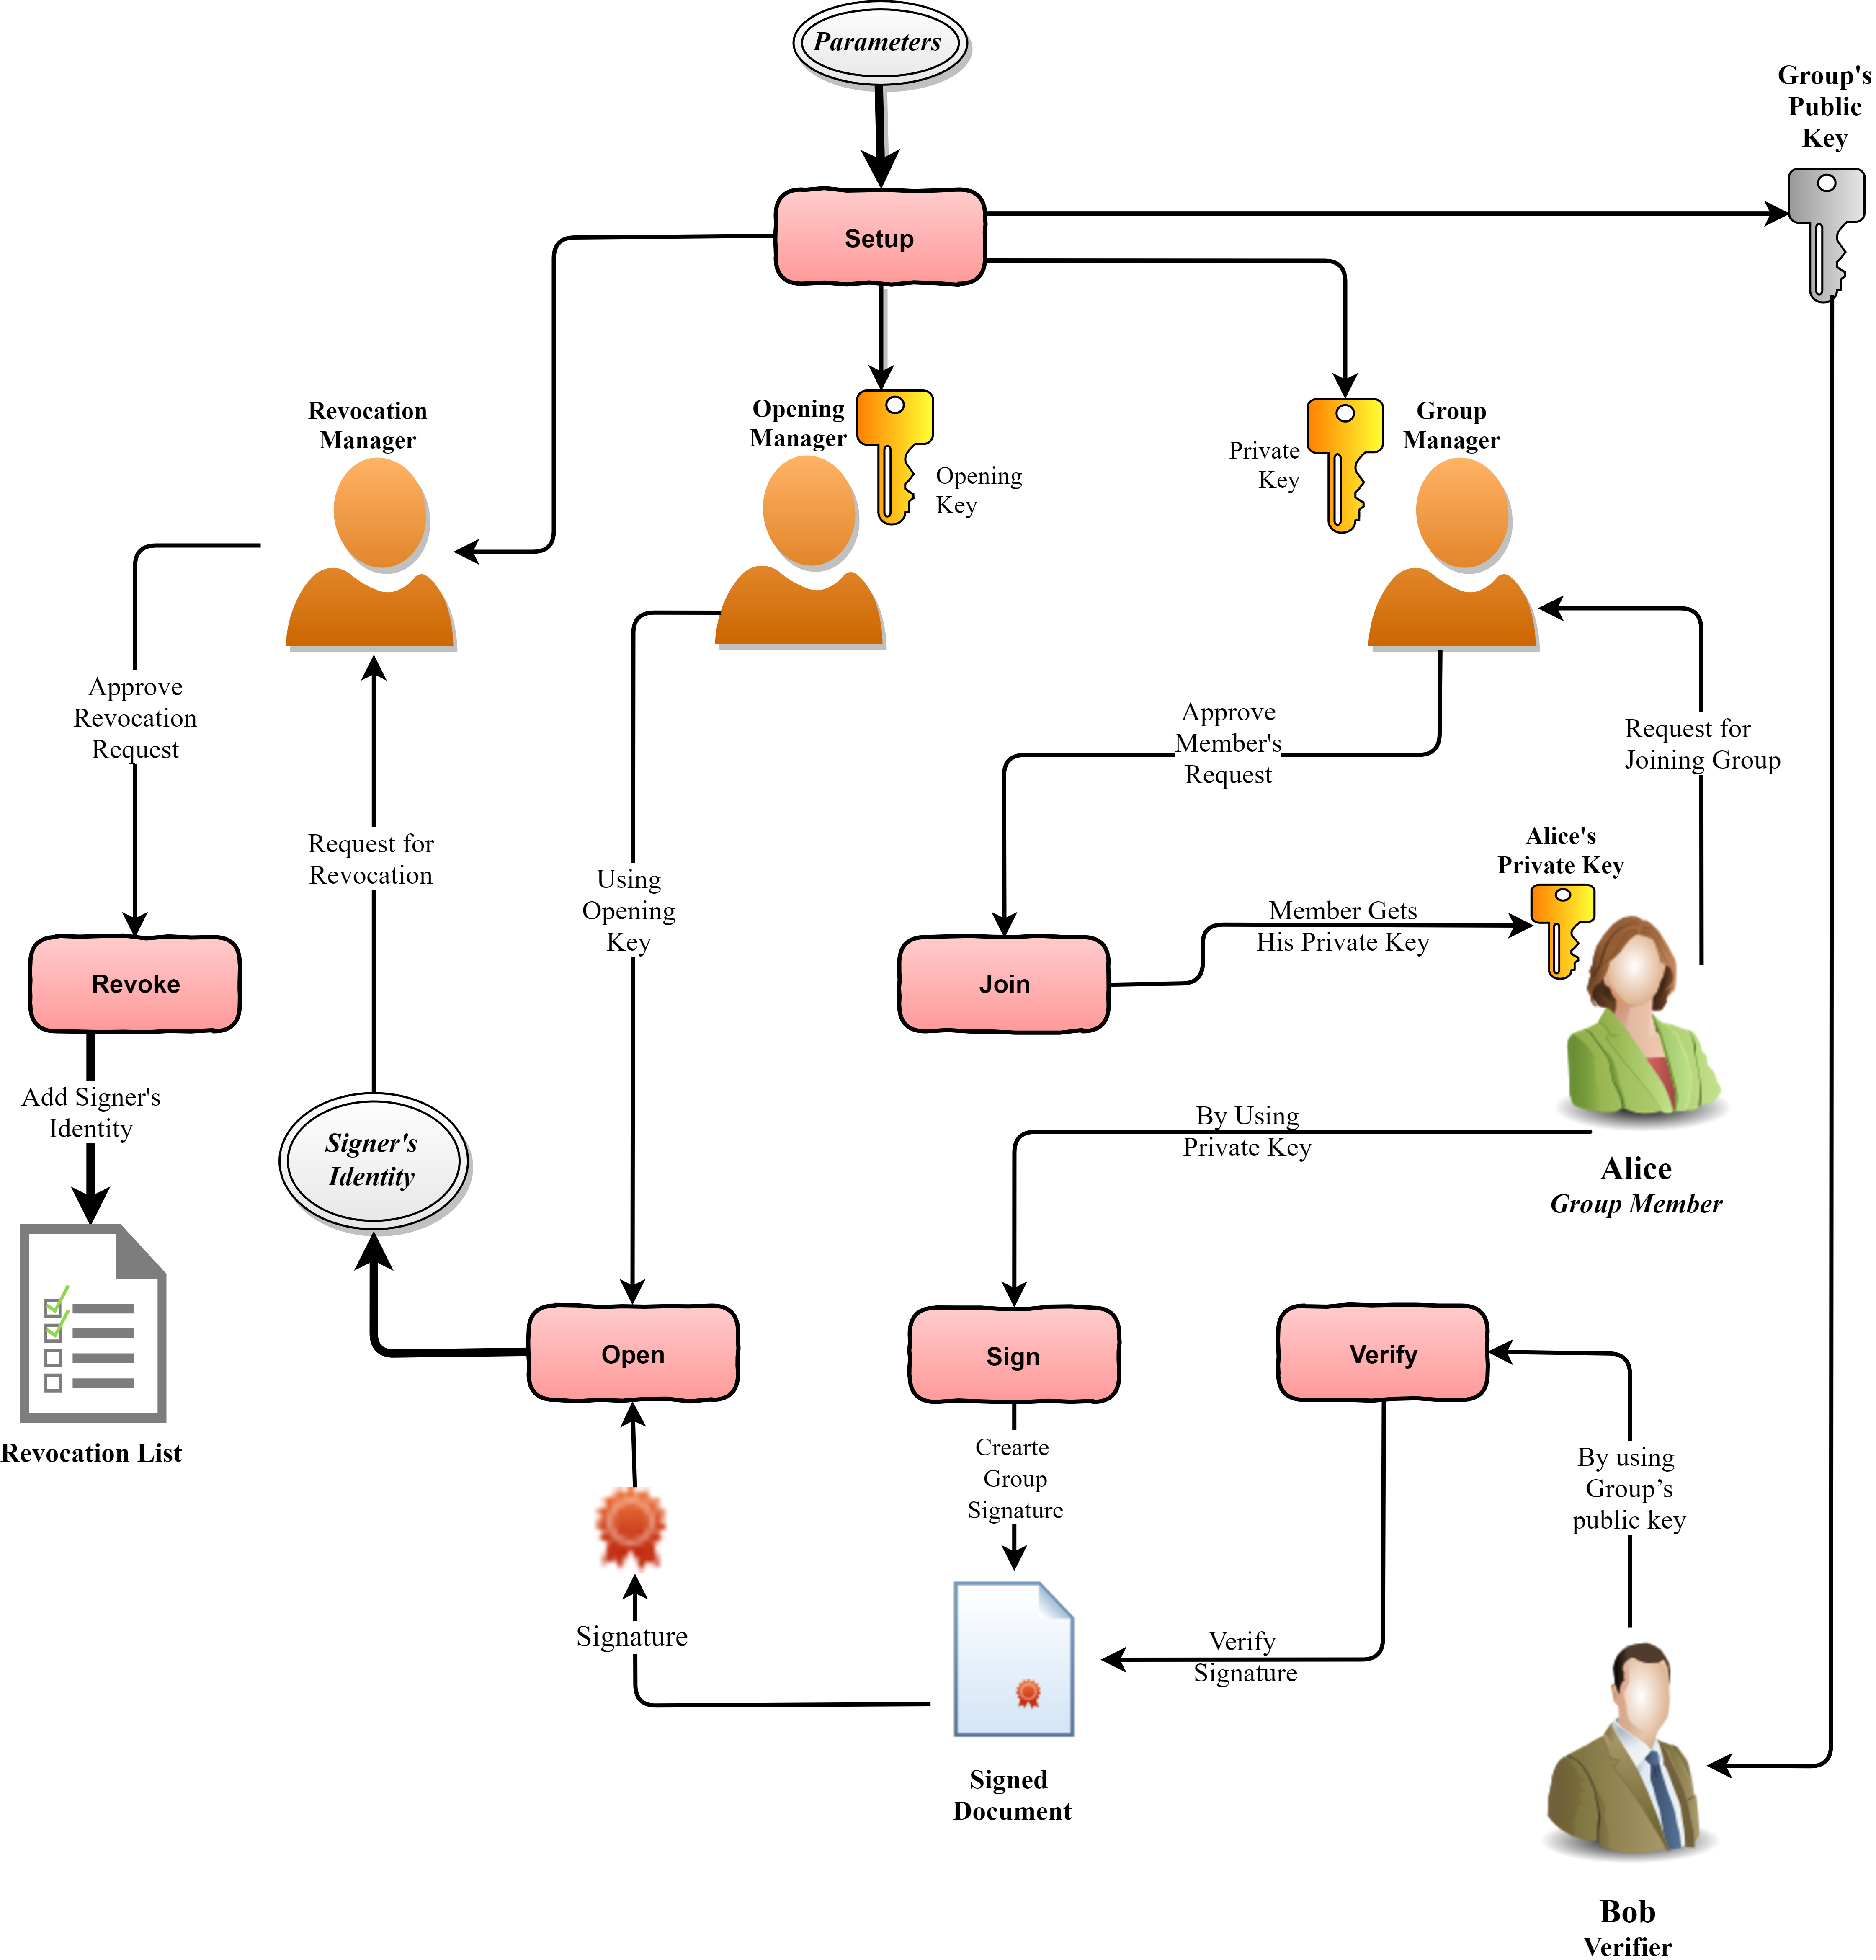
\includegraphics[width=\textwidth]{Architecture_of_group_signature}
    \caption{Architecture of Proposed Group Signatures Scheme}
    \label{fig:Architecture of Proposed Group Signatures Scheme}
\end{figure}

From the definition \ref{def:group signature}, it is simple to understand the system of proposed group signatures scheme. From the figure \ref{fig:Architecture of Proposed Group Signatures Scheme}, we can see that there are three authorities is distributed in this system viz. Group Manager, Opening Manager, and Revocation Manager. The group is started by generating and allocating private keys of the Group Manager and Opening Manager along with the public key of the group. The \texttt{SetUp} algorithm is provided input of the security parameters for generation of those keys. Once the Group Manager and Opening Manager are equipped with their private keys, the group becomes available for potential members to join. 

When a potential member Alice wants to become a member of the group, she sends a request to Group Manager for her addition in the group through the \texttt{Join} protocol. The Group Manager approves the request of the member and calculates some intermediate numbers by using his private key and transmit those numbers to Alice by using \texttt{Join} algorithm from which she can calculate her private key. Note that the private key of Alice is generated at random and the Group Manager does not have knowledge of entire key instead he has a partial knowledge of the key which can act as a unique identification of Alice. The Group Manager stores this identification of Alice in the \textquotedblleft List of group members\textquotedblright.

Once Alice gets her private key by becoming a member of the group, she can sign a message on behalf of the group. To sign a message Alice uses the \texttt{Sign} algorithm which generates a signature when provided with a message and private key of the member. Alice produces a group signature by inputting her private key and her message into the \texttt{Sign} algorithm. The signed message is then ready to be transmitted along with the signature over an insecure channel.

Bob as a non-member user of the group signature system, receives the message signed by a member of the group over an insecure channel. To verify the received message, Bob uses the \texttt{Verify} algorithm which takes an input of the message, its signature and public key of the group. The public key of the group is assumed to be available to Bob because the public key of the group is made available to all the public members either through PKI certificates or direct transmission of the certificates to potential verifiers. When Bob provides input of the received message along with its signature and the public key of the group, the \texttt{Verify} algorithm determines the validity of the signature as either valid or invalid. If the validity of the received message is found to be invalid, Bob discards the message. If the message is verified to be valid, Bob accepts the message. Note that Bob only gets information of validity of the message as is it signed by a valid member of the group or not. But Bob cannot get or determine any other information about actual signer of the message. The \texttt{Verify} algorithm also checks if the signer of the message is revoked. This procedure does not leak any information because of the use of discrete logarithm assumption in the process. If the identity of the signer is found in the \textquotedblleft List of revoked members\textquotedblright, then the \texttt{Verify} algorithm determines the validity of the message as invalid. 

In some rare cases, it is required to find out the identity of the actual signer of a message. In such cases, the message and signature are transmitted to the Opening Manager and requested to determine the identity of the original signer of that message. The Opening Manager who has a secret opening key first checks the validity of message and if the message is valid then proceed to open the message. The Opening Manager utilizes the \texttt{Open} algorithm which takes an input of signature and the private key of the Opening Manager to determine the identity of the signer. The \texttt{Open} algorithm provides the identity of the signer which is then cross referenced with \textquotedblleft List of members\textquotedblright to decide the signer of the signature. The Open Manager is the only authority holding the secret key to determine the identity of the signer. Hence no one except the Opening Manager is able to ascertain the identity of the signer of a signature. The Opening Manager sometimes needs to send the obtained identification to the Revocation Manager to revoke the membership of the signer.

Revocation Manager when received the identification of the signer, can revoke his membership. The Revocation Manager is assigned to the task of determining whether the membership of a member should be revoked or not. The Revocation Manager decides it according to the policy of the group. To revoke the membership, Revocation Manager adds the identification of the signer in the \textquotedblleft List of revoked members\textquotedblright. As we seen in the earlier paragraph, the \texttt{Verify} algorithm also checks the entries of the \textquotedblleft List of revoked members\textquotedblright for the signer while validating a message. So the messages signed by the revoked members are identified as invalid. The \textquotedblleft List of revoked member\textquotedblright is published and made available to all potential verifiers. Only the Revocation Manager have permission to modify that list and other members can only read but cannot edit the list. 

In the next section, we are going to discuss further about the algorithms of the group signature scheme in implementation point of view.

\section{Model Development}
\index{Model Development}From the definition and architecture described in the earlier section, one can see that the proposed group signature scheme is a dynamic group signature scheme with distributed authorities according to the definition \ref{def:Group Signature Scheme with Distributed Authorities} given in section \ref{sec:Group Signature Schemes with Distributed Authorities}.  To develop model according to the architecture and satisfying the definition we need to modify the algorithms and protocols of the group signature scheme. The proposed group signature scheme is based on state of the art ACJT scheme and uses the RSA assumption for its security. In the following section, we are going to describe the modified algorithms of the group signature scheme and their working.

\subsection{Security Parameters}
\index{Security Parameters}The security parameter is a variable which is used to determine the size of the input for a computational algorithm or protocol. The security parameters are used to find out the probability of breaking the security of a cryptosystem. There are several security parameters required for the scheme. Following are some security parameters which are used in various operations of our system. Also, we have used some lengths and ranges which are described below. 

Let the security parameters be $\varepsilon > 1, \ell \in \mathbb{N}, k \in \mathbb{N}$. Let $\lambda_2, \lambda_1, \gamma_2, \gamma_1$ denotes the lengths, and $\Gamma, \Lambda$ denotes integral ranges satisfying following conditions.

\tcbset{float=htb,every float=\centering, colback=white,arc=2mm, equal height group=AT,}
\begin{center}
\begin{tcolorbox}[width= 7cm, height= 7cm, valign = center]
\begin{itemize}
\item $\lambda_2 \geq 4\ell$,
\item $\lambda_1 \geq \varepsilon(\lambda_2 + k) + 2$,
\item $\gamma_2 \geq \lambda_1 + 2$, 
\item $\gamma_1 \geq \varepsilon(\gamma_2 + k)+ 2$,
\item $\Gamma =~]2^{\gamma_1-\gamma_2}, 2^{\gamma_1+\gamma_2}[$,
\item $\Lambda =~]2^{\lambda_1-\lambda_2}, 2^{\lambda_1+\lambda_2}[$.
\end{itemize}
\end{tcolorbox}
\end{center}
The parameter $\ell$ expresses the size of the modulus, and $\varepsilon$ represents tightness of zero knowledge proof. Also, let $\mathcal{H}$ be a collision resistant hash function $\mathcal{H}: \{0, 1\}^* \rightarrow \{0, 1\}^k$.

\subsection{Set Up Algorithm}
\index{Model Development!SETUP}The SetUp algorithm is executed at the very beginning of the group. The SetUp algorithm requires the parameter $\ell$ as an input for deciding the size of factors of RSA modulus $n = pq$ where $p = 2 p^\prime + 1$, $q = 2 q^\prime + 1$ and $p, p^\prime, q, q^\prime$ are all prime integers. The algorithm for SetUp operation is given below.

\begin{algorithm}
\caption{\texttt{SETUP} algorithm}
\begin{algorithmic}[1]
\vspace{10pt}
\STATE Group Manager select a special RSA modulus $n$ by selecting two random $\ell _p$ bit prime $p^\prime$ and $q^\prime$.
\STATE Generate random numbers $g, a, a_0 \in \operatorname{QR}(n)$ and of order $p^\prime q^\prime$.
\STATE Open Manager select a secret random number $x$ of size  $2\ell_p - 1$ and set it as his secret opening key 
\begin{center}
\framebox[1.1\width]{$\mathcal{S}_{om} = (x)$}
\end{center}
\STATE Open Manager get $(g,n)$ from Group Manager and calculate $y = g^x(mod~n)$ and send $y$ to Group Manager.
\STATE Group Manager sets group's public key as 
\begin{center}
\framebox[1.1\width]{$\mathcal{Y} = (n, a, a_0, y, g)$}
\end{center}
\STATE Group Manager sets group's private key as 
\begin{center}
\framebox[1.1\width]{$\mathcal{S}_{gm} = (p^\prime, q^\prime)$}
\end{center}
\vspace{10pt}
\end{algorithmic}
\end{algorithm}

From the above algorithm, we can see that at least Group Manager and Opening Manager are required for execution of SetUp algorithm. The  SetUp of algorithm generates the public key of the group as well as private keys of the Group Manager and Opening Manager. The SetUp operation is required to be executed in trusted manner. Therefore the elements $g, a, a_0$ must be generated by a cryptographically secure random number generator and factorization of $n$ should always be kept in secret. The requirement of elements $g, a, a_0$ in $QR(n)$ is for ensuring trust in the public key of the group without any need of zero knowledge proofs. The private key ${S}_{om}$ is kept secret by the Opening Manager and ${S}_{gm}$ is by Group Manager. The public key of the group is made available through common mediums like certificate signed by a trusted party.
\subsection{Join Protocol}\label{subsec:Joinalgo}
\index{Model Development!JOIN}After generating the public key of the group and private keys of the trusted authorities, the group becomes accessible for potential members to join. The Join protocol is required to be executed using secure communication channels so that any eavesdropper should not be able to get any knowledge of the private key of a member. The algorithm of the Join protocol is as follows.

\begin{algorithm}
\caption{\texttt{JOIN} algorithm}
\begin{algorithmic}[1]
\vspace{10pt}
\STATE User $U_i$ generate random exponent $\hat{x}_i \in_R ]2, 2^{\lambda_2}[$ then send $C_1 = g^{\hat{x}_i}(mod~n)$ to Group Manager. also proves his knowledge of $C_1$.
\STATE Group Manager verifies $C_1 \in \operatorname{QR}(n)$, if verified, then selects $\alpha_i$ and $\beta_i$ $\in_R ]2, 2^{\lambda_2}[$ and sends $\alpha_i$ and $\beta_i$ to user $U_i$.
\STATE User $U_i$ computes
\begin{center}
\framebox[1.1\width]{$x_i = ( \alpha_i \hat{x}_i + \beta_i (mod~2^{\lambda_2})) + 2^{\lambda_1}$}
\end{center}
and sends value of $C_2 = a^{x_i}(mod~n)$.
\STATE Group Manager checks $C_2 \in \operatorname{QR}(n)$. If it is, then selects a random prime $E_i \in_R \Gamma$ and calculate
\begin{center}
\framebox[1.1\width]{$A_i = (C_2 a_0)^{E_i^{-1}} (mod~n)$}
\end{center} 
and sends $U_i$ membership certificate $[A_i, E_i]$.
\STATE Group Manager also Stores $[A_i, E_i]$ in List of group members along with other information of the user $U_i$ like Name.
\STATE User $U_i$ verifies if 
\begin{center}
\framebox[1.1\width]{$a_0 a^{x_i} = A_i^{E_i} (mod~n)$}
\end{center} 
\vspace{10pt}
\end{algorithmic}
\end{algorithm}

From the above algorithm, we can clearly see that the use of zero knowledge protocol authenticates both the Group Manager and members. The member sends request to Group Manager for joining him into the group. Note that the $x_i$ is always hidden from Group Manager instead he only knows $a^{x_i} (~mod n)$ from which calculating $x_i$ is computationally hard. The member also validates the received certificate so no certificate can be issued without knowledge of potential member. The Group Manager also stores the certificate $[A_i, E_i]$ so that identity of user $U_i$ can be obtained later.

\subsection{Sign Procedure}\label{pro:sign}
\index{Model Development!SIGN} A member can generate a group signature for a message after becoming the member of the group by receiving his private key. The generated signature is anonymous and unlinkable to the signer. The following Sign algorithm required an input of the message for which the group signature is being generated and the private key of the member.

\begin{algorithm}
\caption{\texttt{SIGN} algorithm}
\begin{algorithmic}[1]
\vspace{10pt}
\STATE Get input of message $M \in \{0, 1\}^*$ and generate random number $w \in_R \{ 0,1 \}^{2\ell_P}$ and calculate commitments as
\begin{eqnarray*}
\left\lbrace
  \begin{aligned}
T_1 &= A_i y^w (mod~n),\\
T_2 &= g^w (mod~n),\\
T_3 &= T_2^{E_i}(mod~n).
\end{aligned}
  \right\rbrace
\end{eqnarray*}
%**
\STATE Generate random number
$r_1 \in_R \pm \{ 0,1 \}^{\varepsilon(\gamma_2 + k)}$, 
$r_2 \in_R \pm \{ 0,1 \}^{\varepsilon(\lambda_2 + k)}$, 
$r_3 \in_R \pm \{ 0,1 \}^{\varepsilon(\gamma_1 + 2\ell_p + k + 1)}$
and calculate challenges as
%**
\begin{eqnarray*}
\left\lbrace
  \begin{aligned}
d_1 &= T_1^{r_1} / a^{r_2}y^{r_3} (mod~n),\\
d_2 &= T_2^{r_1} / g^{r_3} (mod~n),\\
d_3 &= T_2^{r_1} (mod~n).
\end{aligned}
  \right\rbrace
\end{eqnarray*}
%**
\begin{center}
\framebox[1.1\width]{$C = \mathcal{H}(g|| y|| a_0 || a|| T_1|| T_2|| T_3|| d_1|| d_2|| d_3|| M)$}
\end{center}
and responses as
\begin{eqnarray*}
\left\lbrace
  \begin{aligned}
s_1 &= r_1 - C(E_i- 2^{\gamma_1}),\\
s_2 &= r_2 - C(x_i- 2^{\lambda_1}),\\
s_3 &= r_3 - C E_i w.
\end{aligned}
  \right\rbrace
\end{eqnarray*}
\hfill all in $\mathbb{Z}_n^*.$
\STATE Output generated signature as tuple: 
\begin{center}
\framebox[1.1\width]{$(C, s_1, s_2, s_3, T_1, T_2, T_3)$}
\end{center}
\vspace{10pt}
\end{algorithmic}
\end{algorithm}

The Sign algorithm generates a random number $w$ and calculates the commitments $T_1, T_2$ and $T_3$. From the above algorithm, we can see that the Sign algorithm uses an adaptation of Schnorr identification protocol and signature of knowledge from sections \ref{subsection:Schnorr Identification Protocol} and \ref{subsection:Signature of Knowledge} to produce publicly verifiable signatures. It generates random challenges $d_1, d_2$ and $d_3$ then calculate $C$ a fixed size hash digest of length $k$ from collision resistant hash function. The responses $s_1, s_2$ and $s_3$ are calculated using the private key of members and the calculated hash digest $C$. The employed hash function not only limits the value of  $C$ to a fixed size but also act as a random oracle generating random responses. The signature generated contains the hash digest $C$, commitments $T_1, T_2, T_3$ and responses $s_1, s_2, s_3$ which can be verified by a verifier. Next algorithm shows how this group signature is verified.
\subsection{Verify Procedure}
\index{Model Development!VERIFY}A receiver receives the signed message along with the output of Sign algorithm as a signature, and the public key of the group is also available to the verifier. The description of Verify algorithm which requires the message, its signature and public key of the group is as follows.

\begin{algorithm}
\caption{\texttt{VERIFY} algorithm}
\begin{algorithmic}[1]
\STATE Calculate $C^\prime = \mathcal{H}(g\parallel y\parallel a_0 \parallel a\parallel T_1\parallel T_2\parallel T_3\parallel
\frac{(a_0^C T_1^{s_1-C2^{\gamma_1}})} {(a^{s_2-C2^{\lambda_1}}y^{s_3})}
\parallel \frac{(T_2^{s_1- C2^{\gamma_1}})}{g^{s_3}} 
\parallel (T_2^{s_1-C2^{\gamma_1}}T_3^C
\parallel M) $.
\STATE Signature is valid if and only if $C = C^\prime$ and 
$s_1 \in \{ 0, 1\}^{\varepsilon(k + \gamma_2)+1}$,
$s_2 \in \{ 0, 1\}^{\varepsilon(k + \lambda_2)+1}$,
$s_3 \in \{ 0, 1\}^{\varepsilon(k + \lambda_1+2\ell_p + 1)+1}$.
\IF {Signature is valid}
	\FORALL {$E_i$ in Revocation List}
		\IF {$T_2^{E_i} = T_3$}
			\STATE Output : Signer is Revoked, Signature is Invalid.
			\STATE Break for loop
		\ENDIF
	\ENDFOR
	\STATE Output : Signature is valid.
\ELSE
	\STATE Output : Signature is Invalid.
\ENDIF
\end{algorithmic}
\end{algorithm}

From the above algorithm, we can see that the verify algorithm checks the responses and commitments by recreating challenges $d_1, d_2, d_3$ and generating $C^\prime$ same as $C$ in Sign algorithm but using newly recreated challenges and signature with group public key elements. The comparison of $C$ and $C^\prime$ is used to determine the validity of the signature. The signature is valid if $C = C^\prime$. If the signature is valid then the Verify algorithm cross checks the $T_2^{E_i} = T_3$ for all the $E_i$ present in the revocation list. If one of the equation found to be true, then we can assume that the signer is revoked and the signature is considered to be invalid. The Verify algorithm also uses a hash function as a random oracle. Therefore, it is impossible to generate a duplicate signature. Also, the hash function can detect even the smallest changes to the message and signature elements therefore integrity of message get checked automatically while verifying the signature. 

\subsection{Open Algorithm}
\index{Model Development!OPEN}Sometimes a signature is required to be associated with its original signer. The Opening Manager having a secret key for associating a signature uses the Open algorithm given below. The Open algorithm takes an input of signature and opening key $\mathcal{S}_{om}(x)$.

\begin{algorithm}
\caption{\texttt{OPEN} algorithm}
\begin{algorithmic}[1]
\vspace{10pt}
\STATE Verify the validity of signature by VERIFY algorithm.
\STATE Calculate $A_i$ (The identity of $U_i$) as
\begin{center}
\framebox[1.1\width]{$A_i = T_1/T_2^x$}
\end{center}
\STATE Prove $\log_gy = \log_{T_2}(T_1 / A_i ~mod~n)$.
\vspace{10pt}
\end{algorithmic}
\end{algorithm}

The Open algorithm first verifies the validity of the signature. The Verify algorithm confirms correct form of $T_1, T_2$ and authenticates that the signature has only one unique signer for a valid signature. The Open Manager calculates the $A_i$ of signer $U_i$ as his identity and cross check with List of group members to extract information of the user. The Opening Manager also proves that the extracted $A_i$ is correct by providing a zero knowledge proof. Once a signature is open, it does not mean that the signer cannot produce anonymous signature anymore. The Open algorithm only associates one signature at a time, and the extracted $A_i$ is kept secret by the Open Manager to preserve unlinkability to the other signature of the same signer.

\subsection{Revoke Method}\label{pro:revoke}
\index{Model Development!REVOKE}In a real world scenario, the cancellation of group member from the group is necessary. The revocation process not only removes the member from the group but also invalidates all the signatures issued by him. When Opening Manager associates a signer to a signed message, he can also send a request to Revocation Manager to revoke that member along with $[A_i, E_i]$ of the member.

When Revocation Manager decides to cancel a group member, he publishes the $A_i$ and $E_i$ of revoked user $U_i$ in the List of Revoked members. The Verify algorithm also cross check this revocation list for detecting signatures issued by revoked members. The Verify algorithm verifies that if signer of the message is revoked or not, by cross checking for all $E_i$ in Revocation List satisfying
\begin{center}
\framebox[1.1\width]{$T_2^{E_i}=^? T_3(mod~n)$}
\end{center}

If the equation satisfies for a value of $E_i$, then the Verify algorithm outputs that the signer of the message is revoked and signature is invalid. A predefined threshold is defined for the List of revoked members for optimized length. If and when List of revoked members crosses this threshold, the Group Manager reset the group by generating large random number $r$, such that $GCD(r, p^\prime q^\prime) = 1$ and calculate $a^\prime = a^r$, $a_0^\prime = a_0^r$, therefore for a user $i$
\begin{center}
\framebox[1.1\width]{$A_i^\prime = A_i^r = (a^{\prime x_i} a_0^\prime)^{1/E_i}(mod~n)$}
\end{center}

The Group Manager then replaces the group public key elements $a$ to $a^\prime$ and $a_0$ to $a_0^\prime$ redistributes new certificates $[A^\prime_i, E_i]$ to all  non-revoked members of the group.

\section{Implementation}
\index{Implementation}
The implementation of the proposed group signature scheme is made as web service for posting news anonymously as messages. The web service uses the backend of SQLite database and Python programming language. As the group signature scheme requires many big-integer calculations, especially exponential and modular operations, the choice of selecting Python programming language for backend development appears to be superior to other languages. For the front end of the development, the HTML5 and Bootstrap 3 CSS frameworks were used. The Bootstrap 3 provides some outstanding graphic elements and effects. Therefore, it found efficient to design more beautiful and attractive graphic interface.

The structure of implemented group signature scheme is group of authorized journalist and reporters found at the Setup operation. For setup of the group, the Group Manager and Opening Manager choose their private keys and the public keys of the group is generated as a result of setup operation. The group members as a trusted reporters can publish news anonymously, but a verifier can verify these messages as posted by the authorised group member. If the message is shared on social media, the receivers can also verify the received message. As no one can identify the original signer of any message, the identity, as well as the privacy of the signer, remain secure.

\subsection{Registration and Login}
To join the group, a user first needs to register as a new potential member. The following figures shows the registration and login form in the web service.
\begin{figure}[!h]
    \centering
    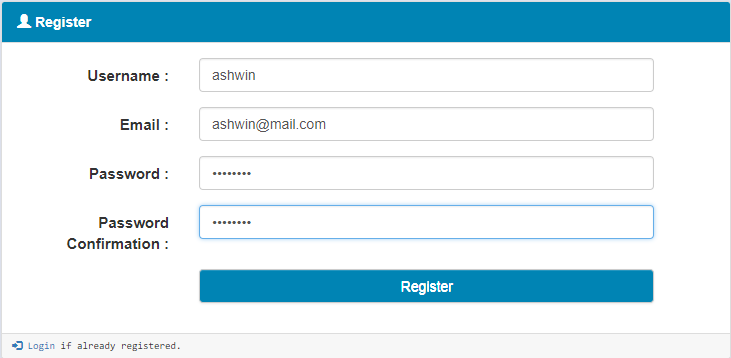
\includegraphics[width=\textwidth]{register}
    \caption{Registration Form}
    \label{fig:Registration Form}
\end{figure}

\begin{figure}[!h]
    \centering
    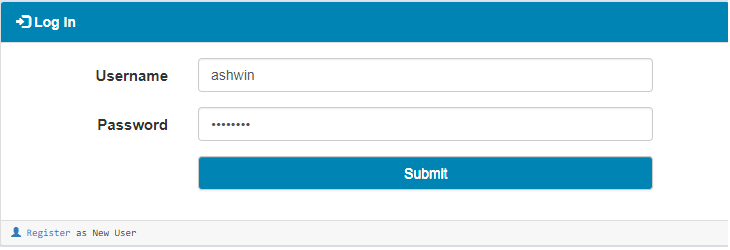
\includegraphics[width=\textwidth]{login}
    \caption{Login Form}
    \label{fig:Login Form}
\end{figure}
The registration is done by getting essential information from the user like name, email id, and password. This information is stored in the database for later reference. At the time of login, the user needs to enter his credentials like username and password for creating a login session. The username and password are compared for authentication of the user. A modern secure method of salted hashing is used to store and compare passwords in the implementation to protect password from intruders and eavesdroppers. This approach is briefly discussed in the following section.

\subsubsection{Salted Hash Passwords}
Storing passwords directly into the database is no longer remain secure as a single breach to the unsecured database by an intruder, or a hacker can lead to the breakdown of the whole implementation as passwords of all the users are known to the hackers. Encrypting the database is also not secure as it can be decrypted by various techniques simplest of it is just stealing it from the person who knows it. Also, persons having access to the database can masquerade as a different user and system do not remain secure. Simple hashing of the passwords is also not secure because of the availability of rainbow tables which contains hashes of common passwords and strings. Therefore, the concept of salted hashing is found to be most secure.

In this technique, the password of the user is first combined with some random strings called as salt. The hash of this combined string along with the salt is stored in the database. Note that the use of an HMAC for hashing is considered more secure as it requires a secret key for hashing. For authenticating a user, the password provided by him is joined with the salt, and its hash is calculated. This calculated hash it now compared with stored hash and if both the strings are equal then the password given by the user is considered as correct. This technique is resistant to brute force attack, and rainbow tables as random salt make it impossible to precompute all the possible hashes. Also by accessing the database, no one can get the passwords hence login system remains secure.

\subsubsection{Joining the Group}
Once the user gets logged in, he can formally join the group by obtaining his private key. To join the group the user clicks on the join link provided on the navigation bar. This initiates the join protocol between the user and Group Manager resulting the member getting his private key. The join operation in the implemented system is completely automatic, and only a single click is required by the user for joining the group. Once the user becomes member of the group, he can post his message in the forum by signing them.
\begin{figure}[!h]
    \centering
    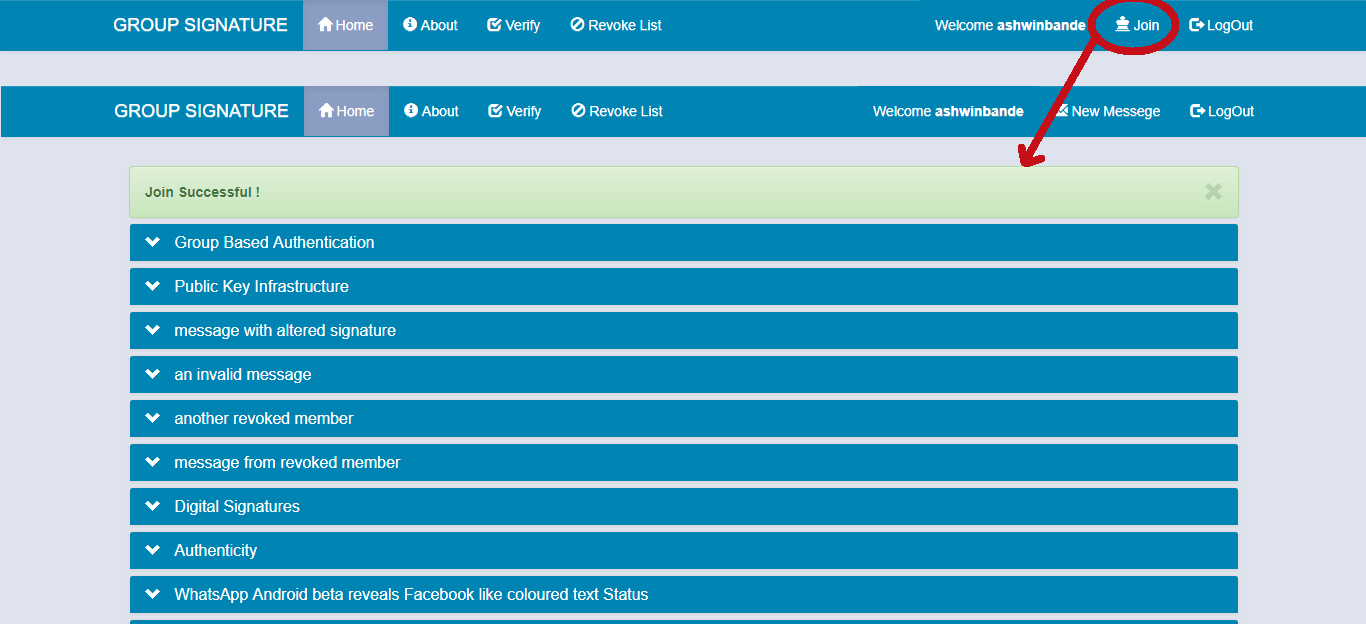
\includegraphics[width=\textwidth]{join_algorithm}
    \caption{Joining Procedure for a New Member}
    \label{fig:Joining Procedure}
\end{figure}

\subsection{Sign and Post}
To publish a message, the member first clicks on the new message and then provide the title and content of the message and click on the sign and post button. This action executes the Sign algorithm where the message and private key of the member are inputted, and the group signature for the message is calculated. The generated group signature along with the message is now published on the homepage of the website. This message can also be shared through various sharing medium like social media or through JSON\nomenclature{JSON}{JavaScript Object Notation} like data interchange format without any need for encryption. The verification of these signed messages is explained in the next section.
\begin{figure}[!h]
    \centering
    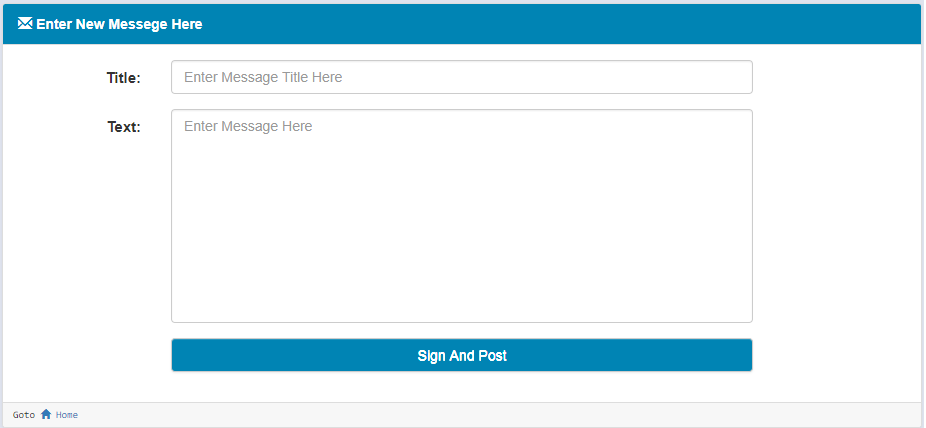
\includegraphics[width=\textwidth]{sign_and_post}
    \caption{Signing and Posting a New Message}
    \label{fig:Signing and Posting a New Message}
\end{figure}

\subsection{Verification}
\begin{figure}[!h]
    \centering
    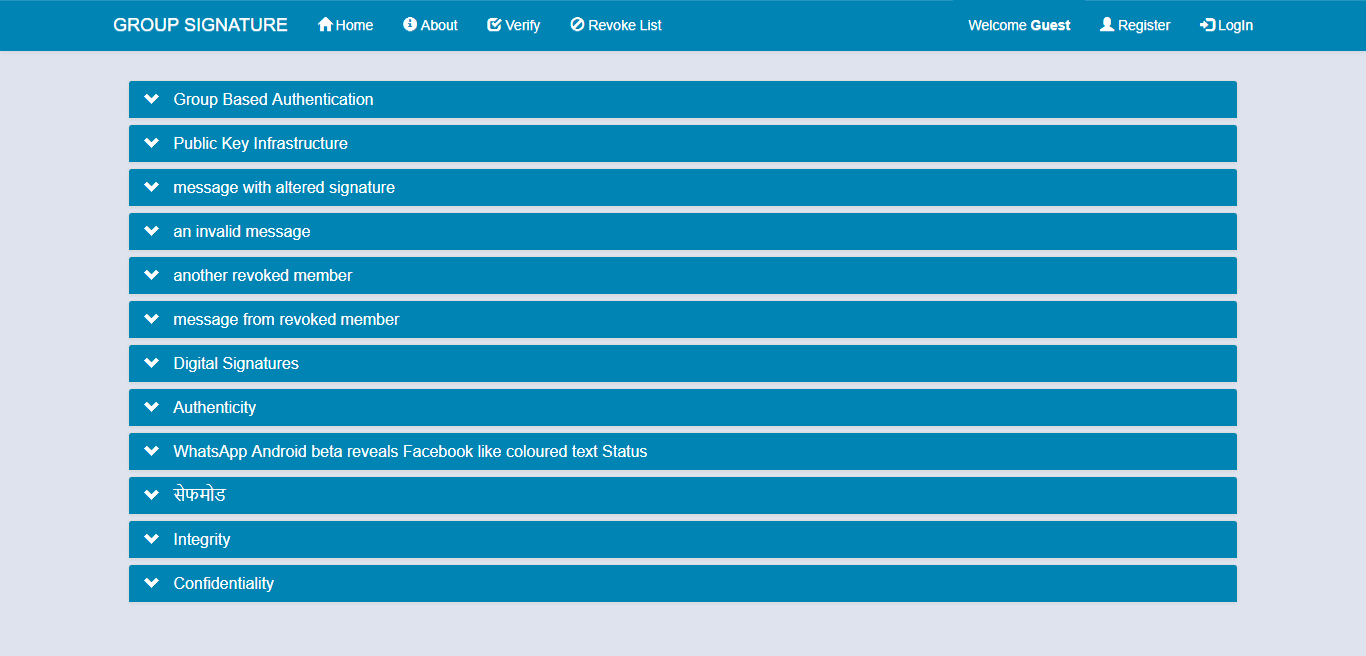
\includegraphics[width=\textwidth]{Homepage}
    \caption{Homepage of the Web Site}
    \label{fig:Homepage of the Web Site}
\end{figure}
Any verifier who wishes to verify a posted message can check it directly on the homepage. Each message contains a verify button that executes the Verify algorithm which takes an input of messages and its signature. The verifier only gets knowledge of the validity of the message as valid or invalid, but no other information is revealed during this procedure.
\begin{figure}[!h]
    \centering
    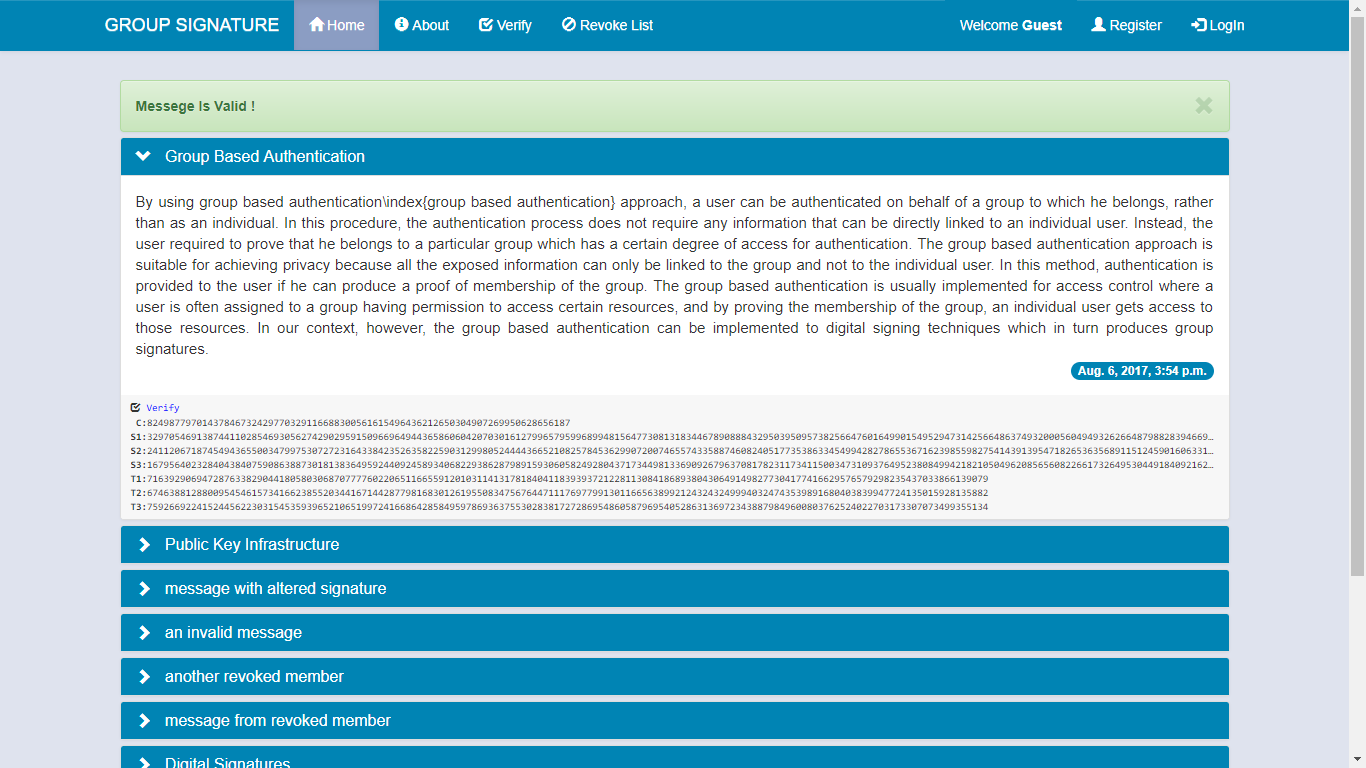
\includegraphics[width=\textwidth]{verified_message}
    \caption{Verification of a Message}
    \label{fig:Verification of a Message}
\end{figure}


\subsubsection{Revocation List}
List of revoked members is published on the web service. This list is publicly accessible and contains identities of revoked members. The Verify algorithm also cross check the signatures with this list to decide whether the revoked member signs a given signature or not. The revocation list is only accessible to the public as read only. The Revocation Manager is the only authority having the write access to the revocation list.
\begin{figure}[!h]
    \centering
    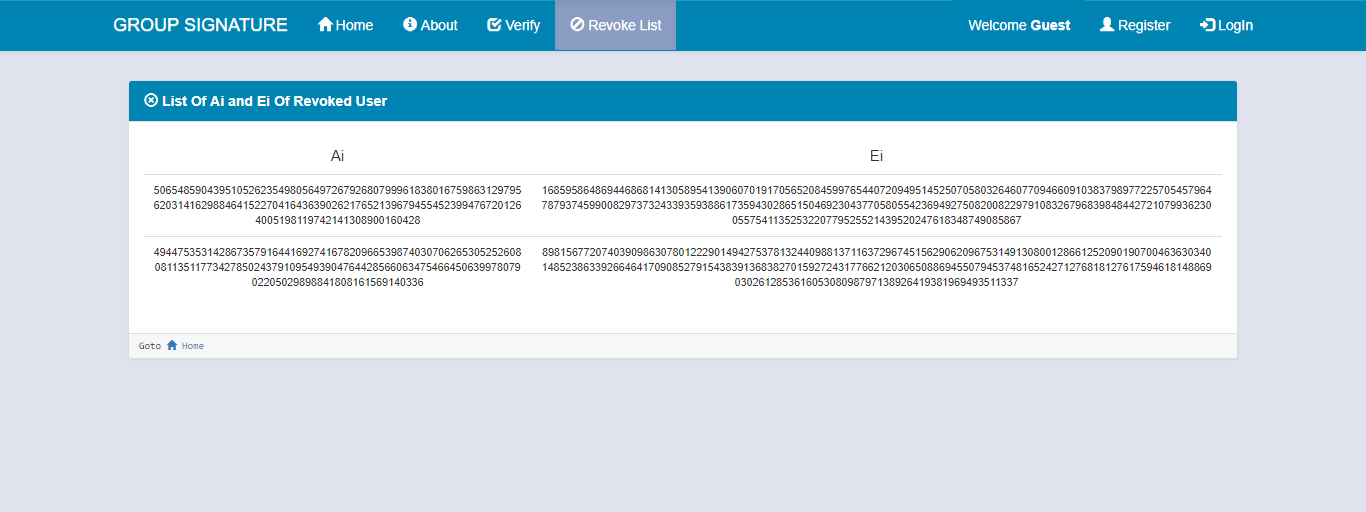
\includegraphics[width=\textwidth]{revocation_list}
    \caption{List of Revoked Members}
    \label{fig:List of Revoked Members}
\end{figure}

\subsection{Opening a Signature}
\begin{figure}[!h]
    \centering
    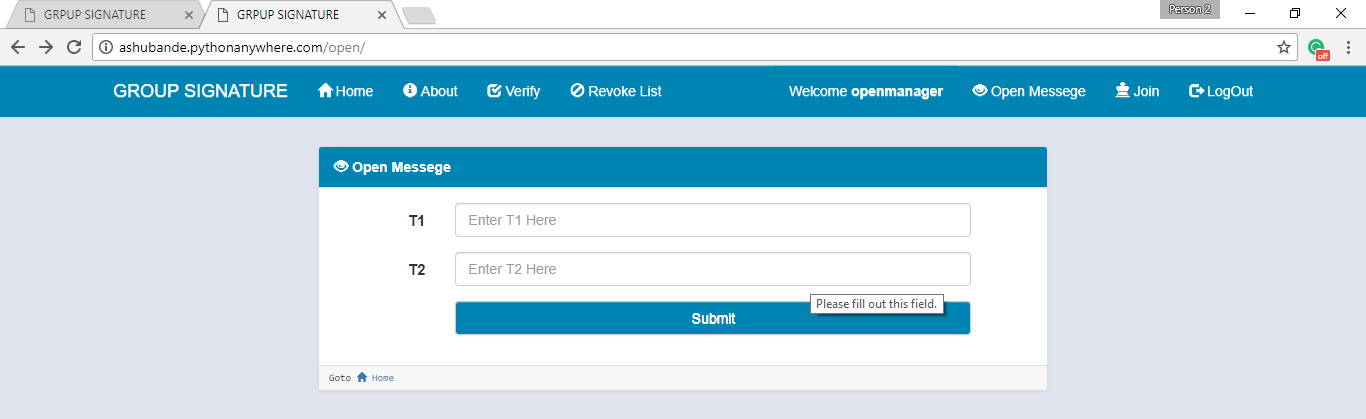
\includegraphics[width=\textwidth]{Opened_form}
    \caption{Form for Opening a Signature}
    \label{fig:Form For Opening a Signature}
\end{figure}
Sometimes the signer of a signature is needed to be identified. The Opening Manager having a specific opening key can associate a particular signature to its unique signer. The Opening Manager is provided with an exclusive option to execute the Open algorithm,  which displays a form. The form takes an input of elements $T_1, T_2$ of the signature and displays computed identity of its unique signer. The Opening Manager then can send a request for revocation of that member to the Revocation Manager. The request contains the calculated identity of the signer.
\begin{figure}[!h]
    \centering
    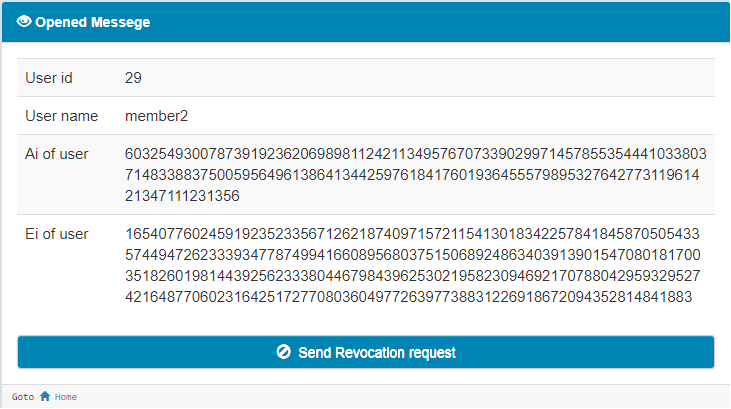
\includegraphics[width=\textwidth]{Opened_messege}
    \caption{Opened Signature of a Message}
    \label{fig:Opened Signature of a Message}
\end{figure}
\subsection{Revocation}
The Revocation Manager when receives the request of the revocation from the Opening Manager, can revoke that member. The Revocation Manager decides whether a member should be revoked or not according to the policy of the group. The Revocation Manager has two options as to accept or decline the request. If the Revocation Manager accepts the request, then the identity of the member received by the Revocation Manager is added to the list of revoked members and the Verify algorithm identifies all the message signed by that member as invalid. 
\begin{figure}[!h]
    \centering
    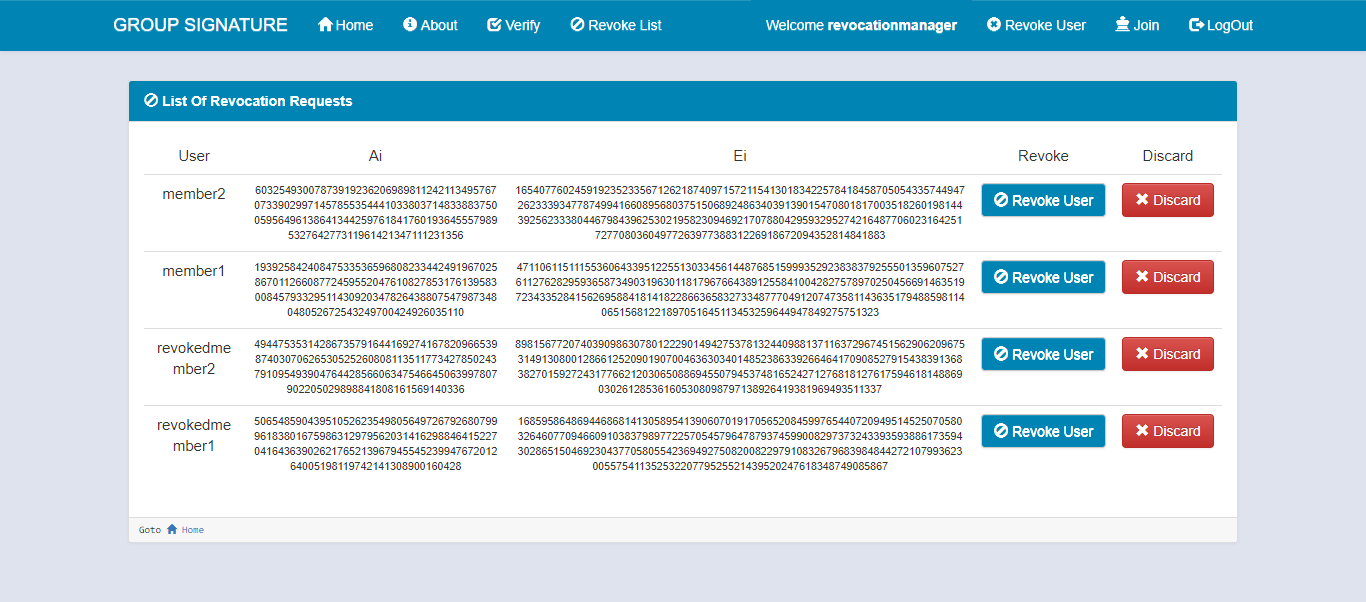
\includegraphics[width=\textwidth]{revocation_requests}
    \caption{Revocation Requests from Opening Manager}
    \label{fig:Revocation Requests from Opening Manager}
\end{figure}


\chapter{Performance Analysis}
%Security and Performance analysis
In the earlier chapter, we have discussed the architecture and implementation of proposed group signature scheme. This chapter analyzes the security and performance of the implemented group signature scheme along with an overview of the functionalities is provided by the implemented scheme and its advantages compared with other similar group signature scheme. Then we will discuss the security properties provided by the scheme and their limitations. The computational cost analysis from authorities and members along with verifiers point of view is also provided in this chapter. The subsequent section presents an overview of functionalities of implemented group signature scheme.

\section{Functionality Overview}
\index{Functionality Overview}
A vast number of facts needed to be analyzed for choosing a suitable group signature scheme for an application. The features like dynamic ness, verifiable opening, distribution of authorities and ability of revocation mechanism are some of the essential functions a group signature scheme must possess. In this section, we are discussing the functionalities provided by the implemented group signature scheme and comparing it to the most notable group signature schemes discussed in Chapter \ref{chp:lit.survay}. Those schemes are divided on the basis of primary cryptographic assumption used for their implementation.

\subsection{Dynamic Behaviour}
\index{Dynamic Behaviour}
The dynamic group signature schemes capable of dynamic addition of members are considered more secure and advanced than the static group signature scheme. Though, static group signatures can be modified to show dynamic behavior. It can be done by precomputing and storing the private keys of the members and allocating them to the members at the time of their joining. This technique has certain security limitations like the precomputed keys are needed to be stored securely by the authority. Also, the authority knowing all the keys can create various attacks like forgery or be framing a member. The dynamic group signature scheme does not have these vulnerabilities and does not require to estimate the number of potential members before the creation of the group.

The implemented group signature scheme is also a dynamic group signature scheme according to the definition provided in section \ref{sub:Dynamic Group Signatures}. The need of pre-computing the private keys of the estimated potential members is not required in this system instead any number of members can join the group at any time. Theoretically, there is always an upper bound present which indicates the maximum possible number of members that can be added to the group. The implemented group signature scheme can add $2^\ell$ members and for a least secure security parameter $\ell$ it can support hundreds of billion possible members. 

From the join algorithm of the implemented group signature scheme discussed in section \ref{subsec:Joinalgo} we can see that the private key of the member is not known to anyone except the member. Even the Group Manager knows a partial key which can only identify the member and used to revoke the membership but not sufficient to forge a signature for framing a member. Therefore the common attacks like framing are not possible in implemented group signature scheme. The join protocol of this scheme is based on the join protocol of ACJT scheme which is considered most secure in the literature of group signature schemes. Therefore the implemented group signature not only have a dynamic behavior but also possess a state of the art security for joining new members. 

\subsection{Distributed Authorities}
\index{Distributed Authorities}
For many groups signature schemes, the Group Manager is single authority responsible for various operations of the group. The Group Manager is called a trusted authority because it is assumed that the Group Manager would not do any malicious activities. For many applications, the Group Manager having this enormous power threatens the privacy of the users as well as the safety of the scheme. Therefore some group signature schemes utilize the concept of distributed authorities.

In group signature scheme supporting distributed authorities, the task of Group Manager is divided into multiple authorities like a separate authority for opening the signature. This distribution is done in two different ways. First, just distribute copies of the same private key to multiple authorities. Although this sounds simple, it does not provide any security enhancement. The tasks are divided between authorities, but one authority can perform tasks of other authorities by using his private key because all authorities were holding the same private key. Another option is complicated but more secure. In this technique, the private key is separated according to its elements and each authority is provided with a private key made up of specific elements such that each key can performance its designated task but not sufficient to perform work of other authorities. This same approach is utilized in the implemented group signature scheme.

In the implemented group signature scheme, the task of Group Manager is distributed between three different authorities. The Group Manager is only responsible for assigning private keys of the members and joining them into the group. The Opening Manager is responsible for associating a unique signer member for a given signature. The Revocation Manager is responsible for revoking the membership of a group member. Each authority has enough power to perform their duties without any need of other authority but not enough to perform operations of other authorities. Therefore the trustworthiness of the authorities is much more in the implemented group signature scheme than other similar schemes. 

\subsection{Verifiable Opening}
\index{Verifiable Opening}
The verifiable opening functionality provides an additional trust for the opening entity. In many group signature scheme, the task of the opening signature is assigned to an entity of confidence and that authority announces original signer of the signature in question. Although,  the authority is trusted it has an absolute power to frame any innocent member or put the blame on a different member. Therefore the confidence in the opening authority is required to be much higher for the efficient functioning of the group.

A more efficient solution to this problem is the implementation of verifiable opening. The verifiable opening allows the opening entity to generate a zero knowledge proof that he associated correct signer member to the signature. The provision of the verifiable opening allows any external verifier to verify the claim pronounced by the opening entity. This functionality reduces the level of trust required in the opening entity and replaces it with verifiable mathematical proof. 

The implemented group signature scheme also allows a verifiable opening of the signatures. The  Opening Manager who is a separate entity responsible for associating a signature to its original signer also provides a zero knowledge proof that the member he claimed to be associated with a signature is, in fact, the original signer of the signature. Therefore the working of the Opening Manager required less trust in him and the proof provides an undeniable evidence against the signer of the signature.

\subsection{Revocation Support}
\index{Revocation Support}
The ability to revoke a group member from static or dynamic group signature group is an essential functionality. The main grounds for the revocation of the members are lost or stolen private keys and the misbehaving group members who signed false documents. Very few group signature schemes support revocation because of its hard implementation. Instead, other group signature schemes insist upon resetting the group by regenerating public and private keys of the authorities as well as group members. The problem of the solution is, it is more costly as every time a new key is needed to be generated and distributed to the group members when even a single member is revoked.

A more efficient solution is the verifier local revocation. The verifier local revocation approach allows the non revoked member to continue using them for producing a signature. The verifier local revocation generates and publishes a list of revoked members and the Verify algorithm verifies if the members sign a given signature in the list. If the signature is found to be signed by a revoked member, the verify algorithm declares the signature to be invalid. Although this approach is considered to be most practical in many groups signature scheme, it has some shortcomings. The main disadvantage is that once the list becomes large the time required for verification is increases linearly therefore standard operations of verification of signatures needed much more time. 

The implemented group signature scheme also uses verifier local revocation approach to allow the revocation of the group members. But the approach found a perfect middle point between resetting the group and linear incrementing time for verification. The Revocation Manager as a separate authority for revocation adds the identity of the revoked member into the revocation list. The list also has a predefined threshold. When the list crosses this predefined threshold, the Group Manager resets the group public key by just changing some elements so that the private key of any authority need not be replaced or recalculated and redistributes new membership certificates to all non revoked members. The advantages of this approach are that it has all the benefits of previous methods but fewer disadvantages of them. Another advantage is that the Opening Manager can open the signature issued previously before resetting the group. 

\subsection{Comparison with Other Schemes}
The following table shows a comparison between various group signature schemes including implemented scheme according to the functionalities provided by them.

\begin{table}[!h]
\begin{threeparttable}
\renewcommand{\arraystretch}{1.3}
\caption{Comparison of various schemes according to functionalities.}
\label{table:functionalities}
\centering
\begin{tabular}{| >{\arraybackslash}m{1.3in} |>{\centering\arraybackslash}m{0.5in} |>{\centering\arraybackslash}m{0.7in} |>{\centering\arraybackslash}m{0.8in} |>{\centering\arraybackslash}m{1in} |>{\centering\arraybackslash}m{0.9in} |}

%\begin{tabular}{| l | c | c | c | c | c |}
\hline 
\textbf{Group Signature} & \textbf{Static} & \textbf{Dynamic} & \textbf{Verifiable Opening} & \textbf{Distributed Authorities} & \textbf{Revocation} \\ 
\hline\hline

ACJT Scheme			& \xmark & \cmark & \cmark & \xmark & \xmark \\ \hline
TX Scheme		 	& \xmark & \cmark & \xmark & \xmark & \cmark \\ \hline
CG Scheme  		 	& \cmark & \xmark & \xmark & \xmark & \xmark \\ \hline
KY Scheme  		 	& \xmark & \cmark & \cmark & \cmark & \xmark \\ \hline\hline
AM Scheme  		 	& \xmark & \cmark & \cmark & \xmark & \xmark \\ \hline
FY Scheme  		 	& \xmark & \cmark & \cmark & \cmark & \xmark \\ \hline\hline
BBS Scheme		 	& \cmark & \xmark & \xmark & \xmark & \xmark \\ \hline
CL Scheme		 	& \xmark & \cmark & \xmark & \cmark & \xmark \\ \hline
BCNSW Scheme	 	& \xmark & \cmark & \cmark & \xmark & \xmark \\ \hline\hline
Implemented Scheme	& \xmark & \cmark & \cmark & \cmark & \cmark \\ \hline

\end{tabular}
\begin{tablenotes}
\item \cmark -- functionality is available. \hspace{0.5in} \xmark -- functionality is not available.
\end{tablenotes}
\end{threeparttable}
\end{table}

\section{Security Analysis}\index{Security Analysis}
This section provides a detailed analysis of the security of implemented group signature scheme. The security of a group signature scheme is dependent on the number of different security properties possessed by the scheme. The following table shows a comparison of various important security properties of different notable group signatures schemes along with the implemented group signature scheme.
\begin{table}[!h]
\begin{threeparttable}
\renewcommand{\arraystretch}{1.3}
\caption{Security properties of group signature schemes.}
\label{table:securityproperties}
\centering
\begin{tabular}{| >{\arraybackslash}m{1.5in} |>{\centering\arraybackslash}m{0.6in} |>{\centering\arraybackslash}m{0.8in} |>{\centering\arraybackslash}m{0.7in} |>{\centering\arraybackslash}m{0.8in} |>{\centering\arraybackslash}m{0.8in} |}

%\begin{tabular}{| l | c | c | c | c | c |}
\hline 
\textbf{Group Signature} & \textbf{Anon.} & \textbf{Traceabl.} & \textbf{Exculp.} & \textbf{Col. Res.} & \textbf{Revocabl.} \\ 
\hline\hline

ACJT Scheme		 	& full	 & insider & full & full 	 & N/A  \\ \hline
TX Scheme		 	& insider& insider & full & partial  & full \\ \hline
CG Scheme  		 	& full	 & full	   & full & partial  & N/A  \\ \hline
KY Scheme  			& full	 & insider & full & partial  & N/A  \\ \hline\hline
AM Scheme  		 	& full	 & insider & full & partial  & N/A  \\ \hline
FY Scheme  		 	& full 	 & insider & full & partial  & N/A  \\ \hline\hline
BBS Scheme		 	& partial& full	   & full & partial  & N/A  \\ \hline
CL Scheme		 	& full 	 & insider & full & partial  & N/A  \\ \hline
BCNSW Scheme	 	& insider& insider & full & full 	 & N/A  \\ \hline\hline
Implemented Scheme	& partial& insider & full & full 	 & full \\ \hline

\end{tabular}
\begin{tablenotes}
\item \textbf{Anon.} - Anonymity; \textbf{Traceabl.} - Traceability; \textbf{Exculp.} - Exculpability;
\item \textbf{Col. Res.} - Coalition resistance; \textbf{Revocabl.} - Revocability.

\end{tablenotes}
\end{threeparttable}
\end{table}

From the above table, one can conclude that the implemented group signature scheme is found to be a superior and more secure than the other schemes because of the vast number of security properties provided by it. As the scheme is based on the ACJT group signature scheme, full coalition resistance is provided in the scheme.
\subsection{Correctness}
\index{correctness} From the implementation of the group signature scheme we can see that:
\begin{itemize}
\item The signatures generated for messages are always of constant length.
\item Every valid signature produced by the group member is always validated as valid by the Verify algorithm.
\item The Open Manager can always associate a unique signer to a given signature and claimed signer is always original signer of the signature. 
\end{itemize}
From the above observation, we are able to conclude that implemented scheme has the security property correctness implemented in it.

\subsection{Unforgeability}
\index{unforgeability}
The implemented group signature scheme uses Schnorr identification protocol from section \ref{subsection:Schnorr Identification Protocol} and an adaptation of signature of knowledge (SoK) discussed in section \ref{subsection:Signature of Knowledge}. The Schnorr identification protocol prevents:
\begin{itemize}
\item The verifier to produce a Forged proof provided by the prover.
\item A masquerader to generate a valid proof.
\end{itemize}
The above propositions are proved in the \cite{schnorr1991efficient}. Also from the section \ref{sub:random oracle model}, if the hash function $\mathcal{H}$ indeed behaves as a random oracle and generate hash digests as a random value. It is not possible to predict the output of $\mathcal{H}$. 

Therefore from the statement presented above, we can conclude that the implemented group signature scheme has security property unforgeability and no one other than a valid group member holding a valid private key can generate a signature that gets verified as valid by the Verify algorithm.

\subsection{Anonymity}
\index{anonymity}
For a given valid signature $(C, s_1, s_2, s_3, T_1, T_2, T_3)$ deciding the actual signer of that signature is computationally infeasible to everyone except the Opening Manager holding the secret opening key. The secret opening key generated at starting of the group act as a trapdoor permutation discussion section \ref{sub:Trapdoor Permutations} and the opening key serves as a trap door that can revert a one way function. Moreover, the generated signature is an adaptation of noninteractive zero knowledge protocols which does not reveal any information about the signer. Therefore we can conclude that the implemented group signature scheme has the security property anonymity. 

But for an entity knowing the secret key $[A_i, E_i]$ of a member $i$ can decide whether that member $i$ signed a given signature or not if he tried to find out $T_2^{E_i} =^? T_3 (~mod n)$. Therefore it is clear that implemented signature scheme does not provide full anonymity but instead provide partial anonymity from the notations of Bellare's model \cite{bellare2003foundations}.

\subsection{Unlinkability}
\index{unlinkability}
From Sign algorithm of implemented group signature scheme discussed in \ref{pro:sign}, we can see that each signature generation required four random numbers $(w, r_1, r_2, r_3)$. Therefore deciding whether given two different signatures $(C, s_1, s_2, s_3, T_1, T_2, T_3)$ and $(\tilde{C}, \tilde{s}_1, \tilde{s}_2, \tilde{s}_3, \tilde{T}_1, \tilde{T}_2, \tilde{T}_3)$ were computed by the same signer is computationally infeasible. 

This problem can be seen as a form of discrete logarithm problem in which to link a given signature required to solve and find out $Dlog_y(T_1/\tilde{T}_1)$ and $Dlog_g(T_2/\tilde{T}_2)$ are same or not which is assumed to be impossible form decisional Diffie Hellman assumption provided in section \ref{sub:DDH}.

\subsection{Exculpability}
\index{exculpability}
The definition \ref{pro:definition} states that the group signature scheme having exculpability property has neither a group member nor any group authority like Group Manager can produce a signature that can be traced back to other members signature. Therefore there are two possible cases for framing.

\begin{itemize}
\item Another member produces a signature: Any other member does not know the private key of another member. Therefore generating a signature to frame another member $i$ required knowledge of private key tuple $[A_i, E_i, x_i]$ hence no member can create a valid signature on behalf of member $i$.
\item Group Manager produces the signature: From the Join protocol of implemented group signature scheme discuss in section \ref{subsec:Joinalgo} we can see that the Group Manager have knowledge part of private key tuple $[A_i, E_i]$. Therefore to generate a signature which can be traced as a signature of member $i$, the Group Manager required to calculate $x_i$ of member $i$. From the Join protocol, we can see that the Group Manager only have knowledge of $C_2 = a^{x_i}(mod~n)$, therefore, the Group Manager required to solve $\log_a C_2$ to calculate $x_i$ which is assumed to be impossible from computational Diffie Hellman assumption provided in section \ref{sub:CDH}. 
\end{itemize}
Therefore we can conclude that even the Group Manager fails to calculate response $s_2$ and cannot generate a valid signature for framing member $i$.

\subsection{Traceability}
\index{traceability}
For a valid signature verified by the Verify algorithm, it can be concluded that the commitments $T_1$ and $T_2$ are in correct form and hence only lead back to $A_i$ of a unique member, if the secret opening key $\mathcal{S}_{om} = (x)$ is known. Therefore the Opening Manager can always obtain $A_i$ of user $U_i$ for every valid signature. Thus we can conclude that the implemented scheme has the security property traceability by which every valid signature is possible to be associated with its original signer member $U_i$.

\subsection{Coalition Resistance}
\index{Coalition Resistance}
The implemented group signature scheme uses similar Join protocol as of the ACJT scheme. Hence the proofs of coalition resistance given in \cite{ateniese2000practical} can also be utilized for implemented signature scheme. Therefore we can conclude that if $\mathcal{H}$ is behaves as a true random oracle and produces coalition resistant output, then there is only a negligible probability that any $\mathcal{H}_1 = \mathcal{H}_2$.

\subsection{Revocability}
\index{revocability}
The Revoke procedure of the implemented scheme provided in section \ref{pro:revoke} shows that the List of revoked member contains $E_i$ of revoked member $U_i$. The Verify algorithm checks that $T_2^{E_i} = T_3 (~mod n)$ and therefore it is not possible to generate a valid signature for a member $U_i$ whose $E_i$ in the List of revoked member. The Verify algorithm can quickly verify that a signature is from a revoked member or not while verifying it.

\section{Performance Overview}
Practical use of a group signature scheme often depends on the computational cost required for its execution. The computational cost depends on the assumptions on which the signature scheme is depended like RSA assumption. Also, the extended properties like revocation or verifiable proofs also increase the computational cost of a group signature scheme. The following analysis of group signature schemes estimates the complexity of most costly operations of various groups signature schemes described in literature review along with the implemented group signature scheme. This comparison provides measurement of the efficiency of discussed schemes. The analysis considers modular exponent in cyclic groups and pairing evaluation as of maximum complexity and cost. 
\subsection{Cost for Authorities}
\index{Cost for Authorities}
\begin{table}[!h]
\begin{center}
\begin{threeparttable}
\renewcommand{\arraystretch}{1.3}
\caption{Computational complexity for group authorities.}
\label{table:Computational complexity for group authorities}
\begin{tabular}{| l | c | c | c |}
\hline 
\textbf{Group Signature} & \textbf{SetUp} & \textbf{Join} & \textbf{Open} \\
\hline\hline

ACJT Scheme		  & $1E$ 	  & $\approx 14E$& $\approx 21E$ 		\\ \hline
TX Scheme		  & $1E$	  & $1E$ 		 & $\approx 21E$ 		\\ \hline
CG Scheme  		  & $2E + 4mE$& N/A 		 & $\approx 13E$ 		\\ \hline
KY Scheme  		  & $2E$	  & $2E$		 & $\approx 17E$ 		\\ \hline\hline
AM Scheme  		  & $2E$ 	  & $5E$  		 & $\mathcal{O}(k)E$	\\ \hline
FY Scheme  		  & $2E$ 	  & $\approx 3E$ & $\mathcal{O}(k)E$	\\ \hline\hline
BBS Scheme		  & $3E + 1mE$& N/A 		 & $\approx 20E + 10P$	\\ \hline
CL Scheme		  & $7E$ 	  & $6E + 1P$	 & $\approx 20E + 8P$ 	\\ \hline
BCNSW Scheme	  & $2E$ 	  & $17E+ 1P$ 	 & $4E + 9P + 3mP$ 		\\ \hline\hline
Implemented Scheme& $1E$	  & $14E$ 		 & $\approx 21E$ 		\\ \hline

\end{tabular}
\begin{tablenotes}\footnotesize
\item \textbf{E} - modular exponentiations; \textbf{P} - pairing evaluations; \textbf{k} - output length of a hash function. \textbf{m} - number of group members.
\end{tablenotes}
\end{threeparttable}
\end{center}
\end{table}
The table \ref{table:Computational complexity for group authorities} shows the computational complexity and overhead for the authorities that manage the group. For dynamic group signature schemes, the Join operation is executed between Group Manager and group members. The above table shows the cost for Group Manager. Note that the complexity of Setup algorithm does not matter because it should be executed only once.


\subsection{Cost for Members and Verifiers}
\index{Cost for Members and Verifiers}
The table \ref{table:Computational complexity for group members and verifiers} provides a comparison of efficiencies of various schemes along with implemented group signature scheme regarding the non-authority, i.e., done by members of verifiers operations. Group members execute the Join and Sign algorithms and verifiers execute Verify algorithm. Note that from member’s point of view the Join operation is performed only once and hence does not have much significance for a scheme.
\begin{table}[!h]
\begin{center}
\begin{threeparttable}
\renewcommand{\arraystretch}{1.3}
\caption{Computational cost for members and verifiers.}
\label{table:Computational complexity for group members and verifiers}
\begin{tabular}{| l | c | c | c |}
\hline 
\textbf{Group Signature} & \textbf{Join} & \textbf{Sign} & \textbf{Verify} \\
\hline\hline

ACJT Scheme		  & $\approx 11E$& $\approx 19E$    & $\approx 18E$ 		\\ \hline
TX Scheme		  & $1E$		 & $\approx 17E$	& $\approx 16E$ 		\\ \hline
CG Scheme  		  & N/A			 & $\approx 10E$    & $\approx 12E$ 		\\ \hline
KY Scheme  		  & $0E$		 & $\approx 13E$    & $\approx 14E$ 		\\ \hline\hline
AM Scheme  		  & $6E$ 	 	 & $\mathcal{O}(k)E$& $\mathcal{O}(k)E$	    \\ \hline
FY Scheme  		  & $\approx 5E$ & $\mathcal{O}(k)E$& $\mathcal{O}(k)E$	    \\ \hline\hline
BBS Scheme		  & N/A			 & $12E + 5P$       & $\approx 18E + 10P$	\\ \hline
CL Scheme		  & $2E$ 	 	 & $16E + 4P$	    & $\approx 16E + 8P$ 	\\ \hline
BCNSW Scheme	  & $15E + 3P$ 	 & $4E+ 3P$ 	    & $2E + 5P$   	 	    \\ \hline\hline
Implemented Scheme& $\approx 11E$& $\approx 19E$    & $\approx 18E$ 		\\ \hline

\end{tabular}
\begin{tablenotes}\footnotesize
\item \textbf{E} - modular exponentiations; \textbf{P} - pairing evaluations; \textbf{k} - output length of a hash function. \textbf{m} - number of group members.
\end{tablenotes}
\end{threeparttable}
\end{center}
\end{table}

\subsection{Comparison with ACJT Scheme}
Although the implemented scheme is based on state of the art ACJT scheme, it has some remarkable differences to the ACJT scheme. The implemented scheme is found to be more efficient than the ACJT scheme. The following table shows a comparison between various algorithms of implemented group signature scheme and ACJT group signature scheme.

\begin{table}[!h]
\begin{center}
\begin{threeparttable}
\renewcommand{\arraystretch}{1.3}
\caption{Comparison between the ACJT scheme and implemented scheme.}
\label{table:Comparison between the ACJT scheme and proposed scheme}
\begin{tabular}{| >{\arraybackslash}m{0.8in} | >{\arraybackslash}m{2.4in} | >{\arraybackslash}m{2.4in} |}
\hline 
\textbf{Procedure} & \textbf{ACJT Scheme} & \textbf{Implemented Scheme} 			\\ \hline\hline

SETUP  & Only Group Manager required. & Group Manager and Open Manager required.\\ \hline
JOIN   & Same                         & Same                                    \\ \hline
SIGN   & $r_4,d_4,s_4$ required. %
		 Uses ElGamel Encryption To %
		 Hide $E_i$.  				  & $r_4,d_4,s_4$ not required. %
		 								It Hides $E_i$ as $T_2^{E_i}$           \\ \hline    
VERIFY & No Revocation supported.     & Cross checking with Revocation List.    \\ \hline
OPEN   & Done by Group Manager.       & Done By separate Opening Manager.       \\ \hline
REVOKE & Not Supported                & Done by Revocation Manager.             \\ \hline \hline
Execution Time & 0.599 Sec.			  & 0.510 Sec  							    \\ \hline
\end{tabular}
\end{threeparttable}
\end{center}
\end{table}

From the above table \ref{table:Comparison between the ACJT scheme and proposed scheme}, it is apparent that the implemented scheme required at least two authorities to produce the public key of the group and the scheme having distributed authorities. The Join operation of ACJT scheme is most secure and efficient. Therefore the implemented scheme adopts the Join procedure same as ACJT scheme except for the use of element $h$. Also the group public key element $h$ is not required in implemented scheme. The Sign operation of implemented scheme reduces the requirement of computing $r_4, d_4, s_4$ and therefore reduce a significant computational cost. Also unlike ACJT scheme, the Sign algorithm does not require any additional ElGamal encryption. The verify algorithm of the implemented scheme also cross-checks with revocation list so the signatures generated by the revoked member should be identified as invalid. Separate opening authority does the opening of signature in implemented scheme. The notable difference between the ACJT scheme and the implemented scheme is the Revoke procedure. The ACJT scheme does not allow revocation of group members whereas implemented scheme have an algorithm which enables revocation of group members by designated revocation authority.

From the Execution time (average) of both the schemes in table \ref{table:Comparison between the ACJT scheme and proposed scheme}, one can clearly see that implemented scheme is about 15\% more faster than ACJT scheme.

\chapter{Conclusion}
In this dissertation, we have proposed an efficient method to implement a dynamic group signature scheme with distributed authorities. The scheme also provides the verifiable opening of the signature. The implemented group signature scheme also enables the secure revocation of group members by using the local verifier revocation technique. The problem of linear incrementation of time required for verification in local verifier revocation is also tackled with an efficient solution of resetting the group. This scheme enhances the privacy of the group members and provides an effective way of identity management. The scheme is practical to implement and proved to be secure under the Diffie Hellman assumption and strong RSA assumption. The scheme also found to be resistant against various attacks like framing, forging or coalition of members. The presented scheme also required less computational overhead compared to other similar schemes. We have shown the effectiveness of our scheme by comparing with state of the art ACJT group signature scheme and almost all important group signature scheme.

\subsubsection{Future Scope}\index{Future Scope}
In future, it can be possible to extend the scheme to practical applications like e-voting and e-bidding. It is also plausible to implement this scheme as a replacement of digital signatures in conceal organizational structures like a company or government departments to provide secure authentication of documents while preserving the privacy of the signer. It is feasible to optimize the revocation technique of the scheme by using some other cryptographic concepts so that the scheme may provide full anonymity instead partial anonymity.
\clearpage

\addcontentsline{toc}{chapter}{References}
\bibliographystyle{ieeetr}
\bibliography{References}

\printindex

\end{document}